\documentclass[12pt,a4paper,oneside]{book} % twoside for draf

%\usepackage{babel}
%\usepackage[T1,T5]{fontenc}
\usepackage[utf8]{vietnam}
\usepackage[utf8]{inputenc}
%\usepackage{times}
%\usepackage{graphicx}
%\usepackage{textcomp}
%\usepackage[backend=biber]{biblatex}

\usepackage[nottoc]{tocbibind}
%\addbibresource{bibbio.bib} % The filename of the bibliography


%\usepackage[english,vietnam]{babel}

\usepackage{array}
\usepackage{floatrow}
\usepackage{comment}
\usepackage{ragged2e}
\floatsetup[table]{capposition=top}
\usepackage[unicode]{hyperref}
\usepackage{tabularx, caption}
\usepackage{caption}
%\setlength{\parindent}{0pt}
\usepackage{indentfirst}
\usepackage{amsmath}
\usepackage{amsfonts}
\usepackage{amssymb}
%\usepackage[]{inputenc}
%\usepackage[francais]{babel}
\usepackage{xcolor}
\usepackage{titlesec}
\usepackage{mdframed}
\usepackage{a4wide,amssymb,epsfig,latexsym,multicol,array,hhline,fancyhdr}
\usepackage{boxedminipage}
\usepackage{amsmath}
\usepackage{lastpage}
\usepackage[lined,boxed,commentsnumbered]{algorithm2e}
\usepackage{enumerate}
\usepackage{color}
\usepackage{graphicx}							% Standard graphics package
\usepackage{array}
\usepackage{tabularx, caption}
\usepackage{multirow}
\usepackage{multicol}
\usepackage{rotating}
\usepackage{graphics}
\usepackage{geometry}
\usepackage{setspace}
\usepackage{epsfig}
\usepackage{tikz}



\usetikzlibrary{arrows,snakes,backgrounds}

\usepackage{tocloft,calc}
\hypersetup{urlcolor=blue,linkcolor=black,citecolor=black,colorlinks=true} 
%\usepackage{pstcol} 								% PSTricks with the standard color package
\usepackage{mathptmx}	% same Time New Roma
%\renewcommand{\rmdefault}{phv} % Arial
%\renewcommand{\sfdefault}{phv} % Arial

\usepackage{fancyhdr}
\usepackage{algorithm2e}
\usepackage{bkthesis}






%\renewcommand\thesubsection{\arabic{subsection}}
\renewcommand\thechapter{\arabic{chapter}}
\renewcommand\thesection{\Roman {section}.}
\renewcommand\thesubsection{\arabic{subsection}.}
%\renewcommand\thesubsubsection{\thesubsection .\arabic{subsubsection}}

\renewcommand{\cftchappresnum}{CHƯƠNG }
\AtBeginDocument{\addtolength\cftchapnumwidth{\widthof{\bfseries CHƯƠNG }}}

%\renewcommand\thesubsection{\arabic{subsection}}

%\csdeptname{KHOA ĐIỆN ĐIỆN TỬ}
%\crname{BÁO CÁO THỰC TẬP TỐT NGHIỆP}
% \crname{BÁO CÁO TIỂU LUẬN}
\title{MỞ RỘNG CHỨC NĂNG CHO MỘT HỆ THỐNG HỖ TRỢ XÂY DỰNG DỮ LIỆU THEO CHUẨN SCORM}	
\cstuname{SVTH:\\1. Nguyễn Duy Minh - 1412279\\2. Tô Thành Nhân - 1412643}


\csCouncil{Khoa học máy tính (Hội đồng 1)}
\csSupervise{TS. Nguyễn Hứa Phùng}
\csReviewer{ ThS. Trần Giang Sơn}
\cttime{6/2018}

\thesislayout



\begin{document}
%-	Bìa cứng - màu xanh dương, chữ mạ vàng (xem mẫu đính kèm)
%-	Trang tên (tờ lót): chất liệu giấy, nội dung giống như bìa LV
%-	Ở gáy LV: in nhan đề LV (có thể in tóm tắt nếu nhan đề quá dài), size 15 – 17
%-	Phiếu Nhiệm vụ LV, chấm điểm Hướng dẫn & Phản biện (đã ký): nhận từ GVHD & GVPB sau khi bảo vệ (theo lịch hẹn).
%-	Lời cam đoan
%-	Lời cảm ơn/ Lời ngỏ
%-	Tóm tắt LV
%-	Mục lục
%-	Danh mục, bảng biểu, hình ảnh, ... (nếu có)
%-	Nội dung LV
%-	Danh mục TL tham khảo
%-	Phụ lục (nếu có)

\coverpage

\frontmatter

% add content here
%-	Lời cam đoan
\begin{declaration}
	\noindent Luận văn của chúng tôi có tham khảo các tài liệu, bài báo, trang web như được trình bày ở
	mục tài liệu tham khảo và ở mỗi tham khảo chúng tôi đều trích dẫn nguồn gốc. Chúng tôi xin cam
	đoan rằng ngoài những trích dẫn từ các tham khảo trên, toàn bộ nội dung trong báo cáo
	là do chúng tôi tự soạn thảo từ những kết quả nghiên cứu của chúng tôi, không sao chép từ bất
	kỳ tài liệu nào khác.\\
	Các số liệu, kết quả nêu trong báo cáo luận văn tốt nghiệp là trung thực và chưa từng được ai công bố trong bất kỳ công trình nào khác.\\
	Chúng tôi xin cam đoan rằng mọi sự giúp đỡ cho việc thực hiện báo cáo luận văn tốt
	nghiệp này đã được cảm ơn và các thông tin trích dẫn trong báo cáo đã được ghi rõ nguồn gốc.\\
	
\hspace{7cm} Sinh viên thực hiện\\

\hspace{5cm}	Nguyễn Duy Minh \hspace{1.5cm} Tô Thành Nhân\\

\end{declaration}

%-	Lời cảm ơn
\begin{acknowledgments}
Để hoàn thành được đề tài luận văn tốt nghiệp này, chúng em đã phải cần đến rất nhiều sự giúp đỡ. Chúng em xin chân thành cảm ơn
\begin{itemize}
	\item Ban giám hiệu nhà trường đã quan tâm và tạo điều kiện thuận lợi cho chúng em học tập và rèn luyện.
	\item Các Thầy Cô Khoa Khoa Học và Kỹ Thuật Máy Tính đã tận tâm giảng dạy, truyền đạt những kiến thức quý báu về công nghệ thông tin, là nền tảng để chúng em thực hiện đề tài luận văn này.
	\item Thầy Nguyễn Hứa Phùng đã truyền đạt cho chúng em kiến thức nền tảng và hướng dẫn chúng em hoàn thành Luận văn Tốt nghiệp này.
	\item Cuối cùng, chúng con xin ghi tạc công ơn nuôi dưỡng và dạy dỗ của Cha Mẹ.
\end{itemize}
Với những kiến thức đã được học ở trường, chúng em mong muốn một ngày nào đó sẽ đóng góp một phần công sức của mình để xây dựng xã hội.
\vspace{1cm}
\begin{flushright}
Sinh viên:\\
Nguyễn Duy Minh\\
Tô Thành Nhân\\
\end{flushright}

\end{acknowledgments}

%
\begin{abstract}
% Tóm tắt luận văn
\end{abstract}	
	
\tableofcontents
%\listofsymbols
\newpage
\listoftables
\newpage
\listoffigures
%\listofalgorithms


\mainmatter

\fancyhead{}  % Clears all page headers and footers
%\rhead{\thepage}  % Sets the right side header to show the page number
%\lhead{}  % Clears the left side page header
%\fancyfoot[positions]{footer}
\renewcommand{\footrulewidth}{0.4pt}

\pagestyle{fancy}  % Finally, use the "fancy" page style to implement the FancyHdr headers

\chapter{GIỚI THIỆU ĐỀ TÀI}

	\fontsize{12pt}{7pt}\selectfont
	\noindent\textit{Chương này sẽ giới thiệu một cách sơ lược về đề tài và cấu trúc của Luận Văn Tốt Nghiệp. Phần đầu của chương sẽ nêu lên tầm quan trọng và ứng dụng của chuẩn SCORM đối với nhu cầu thực tế hiện tại, hệ thống được lựa chọn để phát triển và các chức năng được hiện thực trong phạm vi giới hạn của Luận Văn này. Mục tiếp theo sẽ trình bày cấu trúc của Luận Văn Tốt Nghiệp.}

\section{Tầm quan trọng của đề tài}

	Công nghệ thông tin đang là một lĩnh vực quan trọng của xã hội, vì những ứng dụng thực tế của ngành công nghệ thông tin ngày càng trở nên thiết thực và hữu ích.  Như việc ứng dụng công cụ khai phá dữ liệu vào thương mại điện tử để nắm bắt nhu cầu khách hàng, ứng dụng các mô hình học máy, học sâu vào nhận diện ảnh y khoa, dự báo dòng chảy sông,... Đối với lĩnh vực giáo dục có thể kể đến một ứng dụng rất gần gũi là E-Learning - hệ thống học tập online thông qua việc sử dụng Internet. E-Learning đã cải thiện hoàn toàn hệ thống học tập truyền thống.\\

	Nội dung được hiển thị và trình bày trên E-Learning rất đa dạng và phong phú với nhiều hình thức khác nhau. Các nội dung trên E-Learning có thể ở dạng văn bản, hình ảnh hay video, bài Quiz, các bài kiểm tra với nhiều hình thức khác nhau như câu hỏi trắc nghiệm, tự luận hay điền khuyết,... Người soạn thảo có thể dùng một công cụ biên soạn (Authoring Tool) để xây dựng một bài giảng điện tử, kết hợp nhiều hình thức này với nhau để tạo nên một bài giảng có chất lượng, nội dung phong phú và tránh gây nhàm chán cho người học.\\
	
	Để thực hiện một bài giảng điện tử thì cần phải có hai nhóm công cụ là công cụ để xây dựng bài giảng và công cụ để hiển thị bài giảng. Công cụ xây dựng bài giảng là công cụ giúp người soạn thảo có thể tạo bài giảng và xây dựng nội dung cho bài học. Công cụ để hiển thị bài giảng sẽ hiển thị những nội dung của bài học mà người soạn thảo đã xây dựng cho bài giảng, giúp người học có thể tương tác với những nội dung này.
	
	\begin{center}
		\begin{figure}[htp]
			\begin{center}
				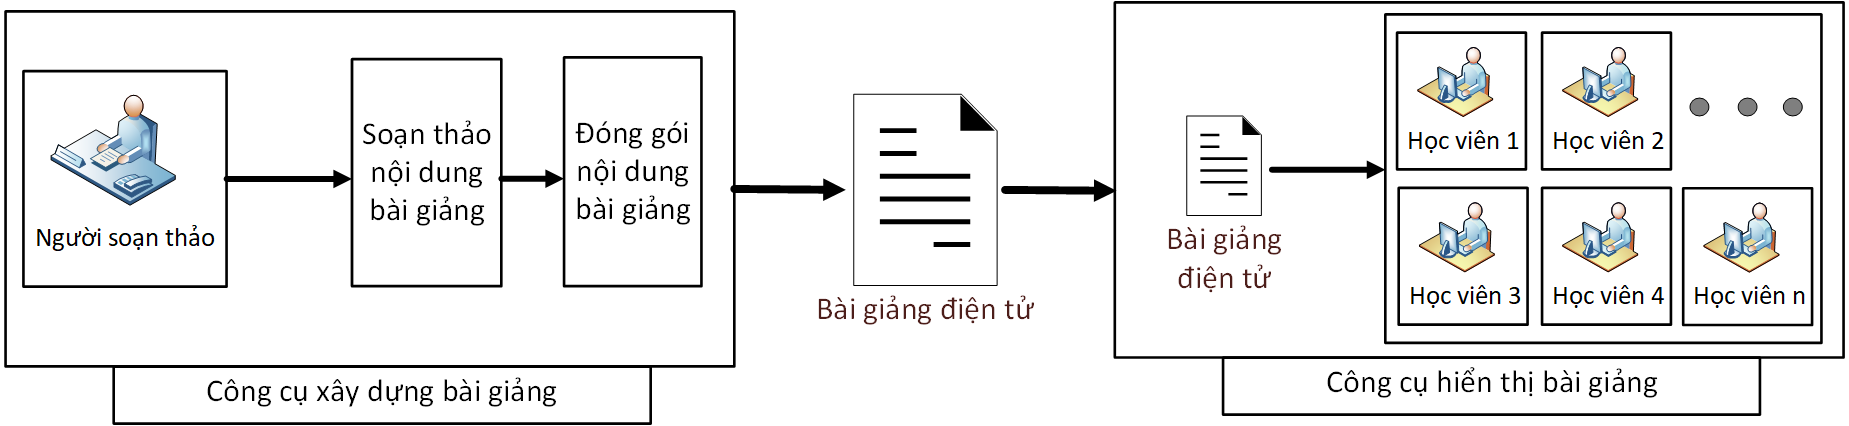
\includegraphics[width=16cm]{Chapter1/Pictures/picture11.png}
			\end{center}
			\caption{Mối quan hệ giữa công cụ xây dựng và hiển thị bài giảng}
			\label{picture11}
		\end{figure}
	\end{center}
	
	\newpage
	
	
	Hình \ref{picture11} thể hiện mối quan hệ giữa công cụ xây dựng bài giảng và công cụ hiển thị nội dung bài giảng. Người soạn thảo sẽ sử dụng công cụ xây dựng bài giảng để tạo bài giảng, xây dựng nội dung cho bài giảng và đóng gói các nội dung này. Sau đó công cụ hiển thị bài giảng sẽ hiển thị nội dung của bài giảng này và giúp người học có thể tương tác với những nội dung của nó.\\
	
	Để hai công cụ này có thể làm việc được với nhau cần có một chuẩn dữ liệu chung, tương thích với cả hai công cụ này. Khi đó các dữ liệu trao đổi giữa hai công cụ này phải tương tác được với nhau, từ đó phát sinh nhu cầu cần có một chuẩn đóng gói dữ liệu giúp hỗ trợ cho việc tương tác giữa hai công cụ này. Có rất nhiều chuẩn đóng gói hiện nay hỗ trợ vấn đề này, trong đó SCORM là một chuẩn như vậy. Chuẩn SCORM là một chuẩn đóng gói bài giảng E-Learning phổ biến nhất hiện nay, được phần lớn các tổ chức sử dụng và chi tiết về chuẩn SCORM sẽ được trình bày trong chương tiếp theo.\\
	
	
	Trong giai đoạn Đề Cương Luận Văn Tốt Nghiệp, nhóm đã tiến hành khảo sát một số SCORM Builder (công cụ soạn thảo có hỗ trợ chuẩn SCORM). Một số SCORM Builder được thương mại hóa như Lectora Inspire 17, Story Line 3, Adobe Presenter,... có độ ổn định cao, cung cấp môi trường soạn thảo đa dạng, tạo được nhiều nội dung tương tác cao với người học và khai thác hoàn toàn thế mạnh của chuẩn SCORM hiện tại. Tuy nhiên, các công cụ thương mại này thường có giá thành rất cao và không có mã nguồn để tham khảo. Bên cạnh đó cũng có một số SCORM Builder có mã nguồn mở như eXe, LAMS, Reload Editor,... Các SCORM Builder có mã nguồn mở cũng có hỗ trợ chuẩn SCORM, cung cấp môi trường soạn thảo,... nhưng các chức năng của chúng vẫn còn hạn chế, chưa khai thác được hết sức mạnh của chuẩn SCORM.\\
	
	
	eXe là một trong số các SCORM Builder có mã nguồn mở hiện nay. eXe hỗ trợ trình soạn thảo có giao diện thân thiện với người dùng, dễ sử dụng, hỗ trợ tạo nội dung bài giảng bằng nhiều hình thức khác nhau như văn bản, hình ảnh hay video,... nó cũng hỗ trợ cho việc tạo bài kiểm tra với nhiều hình thức như câu hỏi trắc nghiệm có nhiều lựa chọn, câu hỏi trắc nghiệm một lựa chọn, điền khuyết,... Tuy nhiên hiện nay chức năng của nó vẫn còn hạn chế, thua xa những SCORM Builder được thương mại hóa khác. eXe giúp người soạn thảo tạo nội dung các bài học, nhưng các bài học này không được quy định thứ tự học, người học có thể ngay lập tức vào học bất kỳ bài học nào có trong bài giảng, điều này sẽ không đảm bảo khả năng tiếp thu của người học. eXe cũng hỗ trợ cho việc tạo bài kiểm tra, nhưng các câu hỏi của bài kiểm tra không có sự phân loại, vị trí các câu hỏi của bài kiểm tra là cố định, điều này sẽ không đảm bảo chất lượng của một buổi kiểm tra vì mọi học viên đều làm các bài kiểm tra có nội dung y hệt nhau.\\
	
	Do đó eXe được nhóm lựa chọn để mở rộng thêm một số chức năng. Chức năng thứ nhất là cho phép người soạn thảo có thể thiết lập thứ tự của các bài học, đưa ra một lộ trình cụ thể cho người học và đảm bảo người học có thể tiếp thu đầy đủ kiến thức của một bài giảng. Chức năng thứ hai là thiết kế một công cụ tạo bài kiểm tra tổng hợp, các câu hỏi trong bài kiểm tra tổng hợp này sẽ có khả năng phân loại độ khó, cuối cùng là vị trí các câu hỏi cũng như câu trả lời của bài kiểm tra này có thể thay đổi được thứ tự ở mỗi lần người học thực hiện. Chi tiết các chức năng được mở rộng sẽ được trình bày ở phần sau.
	
\section{Đề tài luận văn tốt nghiệp}
\subsection{Chức năng điều khiển có điều kiện}

	Hiện tại eXe chỉ hỗ trợ xây dựng bài giảng theo dạng tự do, không có điều kiện. Các bài học trong bài giảng này sẽ không có quy định trình tự học, người học khi bắt đầu tham gia bài giảng có thể ngay lập tức học bất cứ bài học nào có trong bài giảng, kể cả bài cuối cùng mà không cần quan tâm có cần phải học bài nào trước đó hay không. Điều này sẽ không đảm bảo về khả năng tiếp thu kiến thức của người học.
	
		\begin{center}
	\begin{figure}[htp]
		\begin{center}
			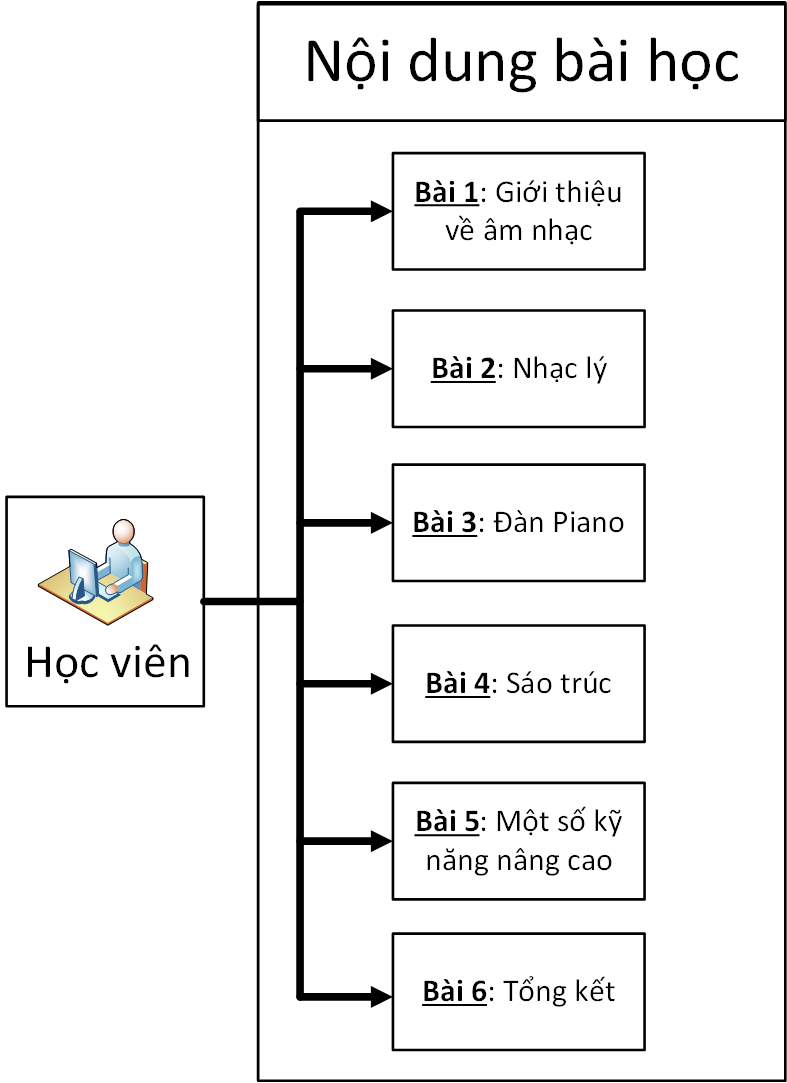
\includegraphics[width=6cm]{Chapter1/Pictures/picture12.png}
		\end{center}
		\caption{Mô hình bài giảng hiện tại của eXe}
		\label{picture13}
	\end{figure}
\end{center}


	
	Hình 1.2 thể hiện ví dụ của mô hình này, khi bắt đầu một bài học, người học có thể di chuyển vào bất cứ bài nào trong một khóa học mà không gặp bất cứ ràng buộc nào. Theo như ví dụ ở hình 1.2 thì người học có thể ngay lập tức học \textbf{Bài 6: Tổng kết}, việc này sẽ ảnh hưởng đến thời gian và hiệu suất học tập của người học, vì nếu như chưa trang bị đủ kiến thức của những bài trước mà lại lựa chọn ngay vào học bài tổng hợp nằm ở cuối cùng thì sẽ không đảm bảo cho việc tiếp thu đầy đủ kiến thức của khóa học.\\
	
	Về mặt chuyên môn, người học cần phải học các bài theo một trình tự khoa học. Trước khi vào học "Bài 2: Nhạc Lý", người học ít nhất cần phải học "Bài 1: Giới thiệu về âm nhạc" trước đó, sau đó "Bài 3: Đàn Piano" phải được học sau "Bài 2: Nhạc lý" vì người học cần phải có kiến thức về nhạc lý trước đó mới có thể học nhạc cụ,... Tuy nhiên eXe chưa hỗ trợ cho việc thiết kế mô hình này. Hình 1.3 thể hiện các bài học được quy định theo một lộ trình cụ thể.
	

	
		\begin{center}
		\begin{figure}[htp]
			\begin{center}
				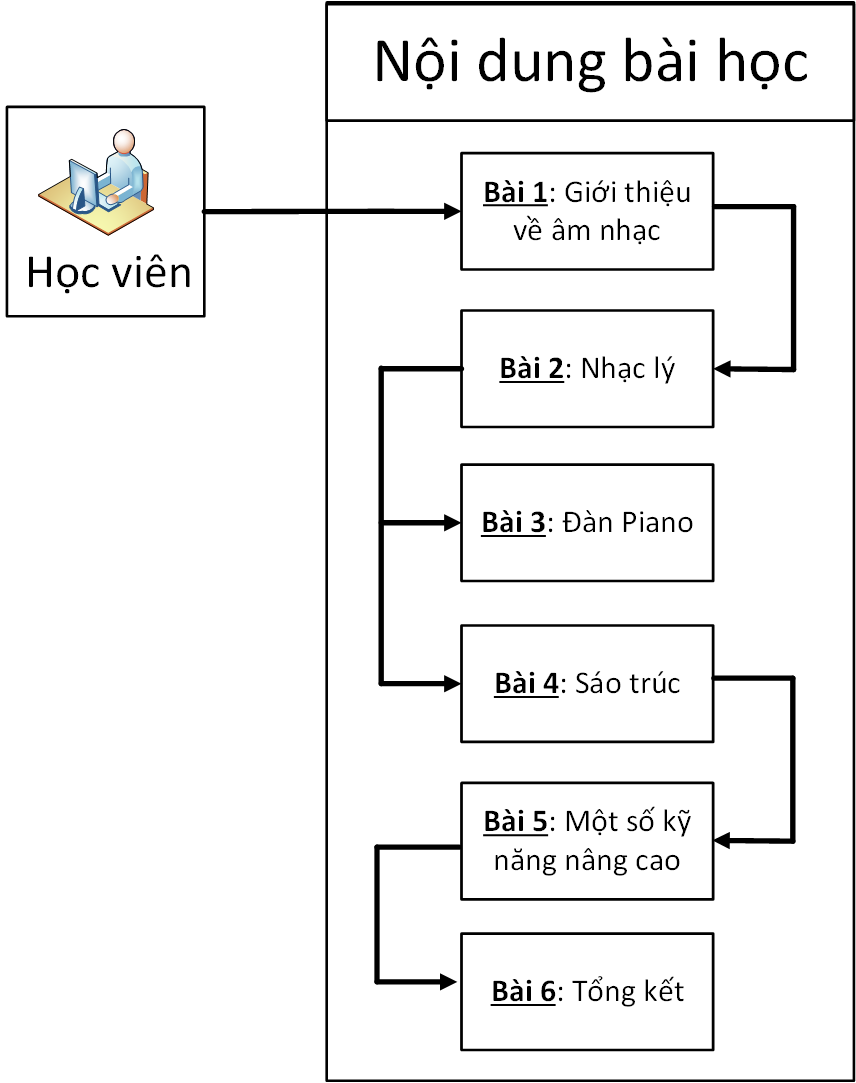
\includegraphics[width=6cm]{Chapter1/Pictures/picture13.png}
			\end{center}
			\caption{Các bài học có thứ tự}
			\label{picture12}
		\end{figure}
	\end{center}
	\newpage
	
	Chức năng điều khiển có điều kiện sẽ giúp người soạn thảo có thể xây dựng bài học như mô hình trên. Chức năng này giúp người soạn thảo có thể thiết lập điều kiện ở mỗi bài, giúp đưa ra một lộ trình học cụ thể. Điều kiện bao gồm tiền điều kiện và hậu điều kiện. Tiền điều kiện là điều kiện mà người học cần thỏa mãn để được vào học một bài học, tiền điều kiện của 1 bài học là bài học mà người học cần phải hoàn thành (thỏa mãn hậu điều kiện) trước khi vào nội dung của bài học này. Hậu điều kiện là điều kiện xác nhận người học đã hoàn thành bài học này, hậu điều kiện có thể là thời gian tối thiểu mà người học phải bỏ ra cho một bài học hoặc phải đạt một số bài kiểm tra nào đó trong bài học do người biên soạn quy định. Sau đây là ví dụ giúp người đọc dễ hình dung hơn.
	
		\begin{center}
		\begin{figure}[htp]
			\begin{center}
				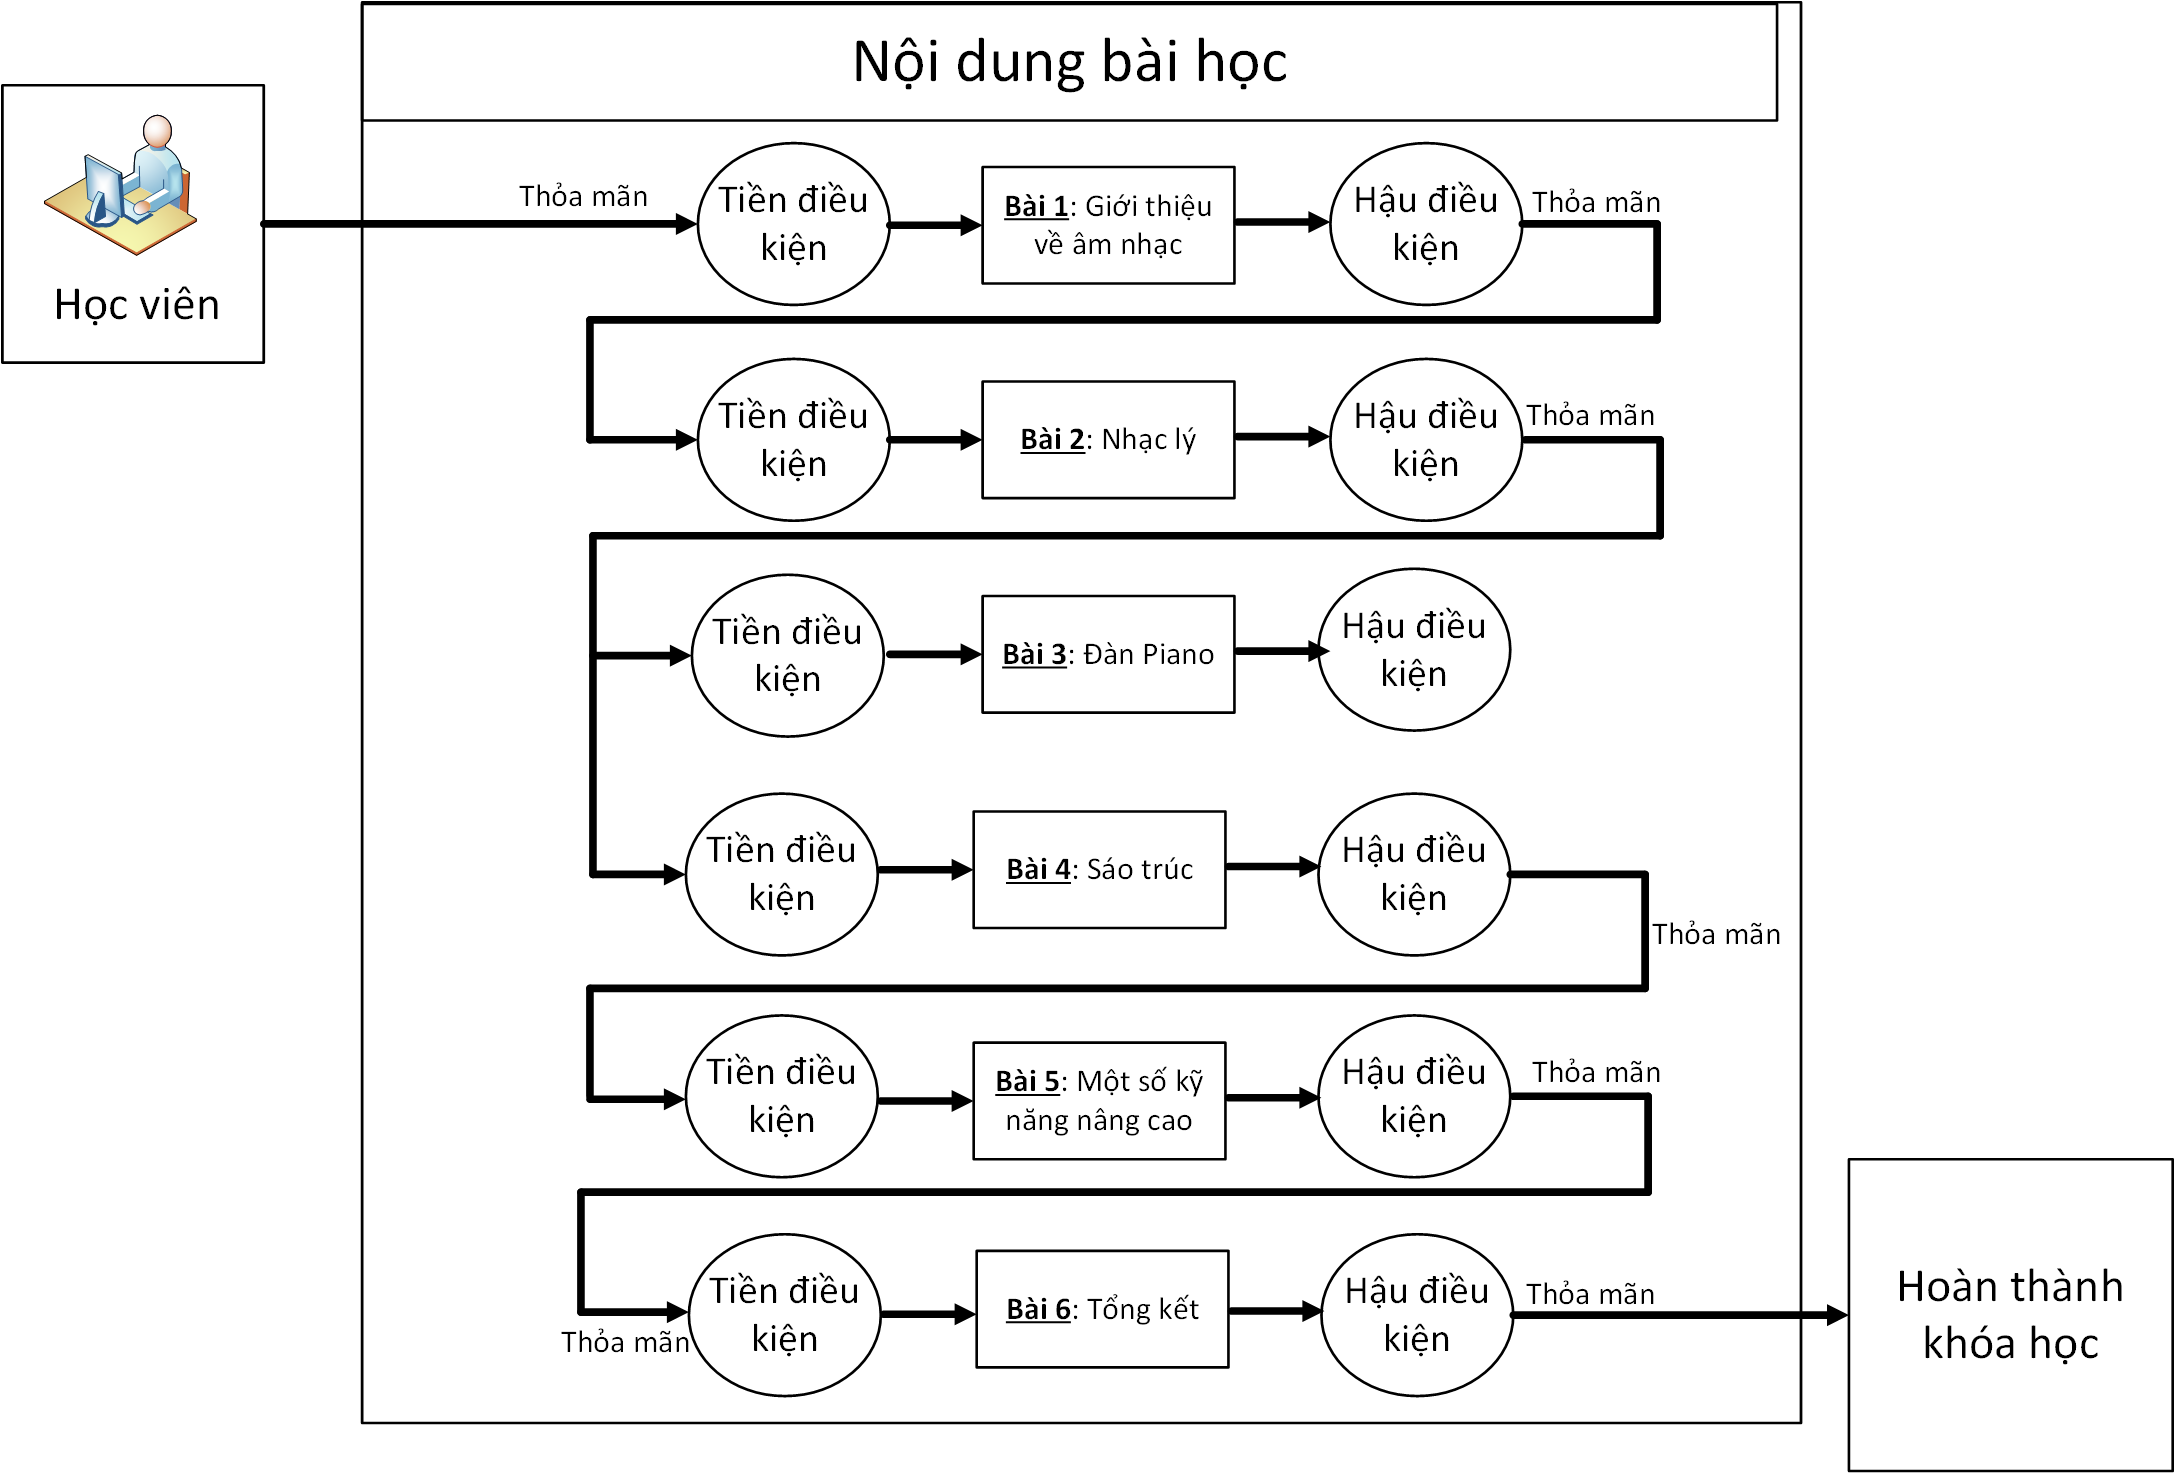
\includegraphics[width=16cm]{Chapter1/Pictures/picture14.png}
			\end{center}
			\caption{Mô hình điều khiển có điều kiện}
			\label{refpicture13}
		\end{figure}
	\end{center}


	Hình 1.4 thể hiện ví dụ một mô hình điều khiển có điều kiện, ở mỗi bài học đều được thiết lập tiền điều kiện và hậu điều kiện tương ứng. Đầu tiên học viên sẽ học "Bài 1: Giới thiệu về âm nhạc", vì đây là bài đầu tiên của khóa học nên sẽ không cần tiền điều kiện. Tiếp theo học viên muốn học "Bài 2: Nhạc lý" thì học viên cần phải thỏa mãn tiền điều kiện của Bài 2 này, tức hậu điều kiện của Bài 1, hậu điều kiện của Bài 1 có thể là thời gian phải bỏ ra hoặc bài kiểm tra cần đạt tùy theo thiết lập của người soạn thảo. Sau khi hoàn thành Bài 2, học viên có thể lựa chọn tiếp tục học "Bài 3: Đàn Piano" hoặc "Bài 4: Sáo trúc", vì nội dung của hai bài này độc lập với nhau. Sau khi hoàn thành "Bài 4: Sáo trúc" thì học viên có thể tiếp tục học "Bài 5: Một số kỹ năng nâng cao" và cuối cùng là "Bài 6: Tổng kết".
	
	
	
	\newpage
	
\subsection{Chức năng tổng hợp câu hỏi và tạo bài kiểm tra}
	
	Trong việc thiết kế một bài giảng điện tử, nhu cầu kiểm tra kiến thức của người học sau mỗi bài học là rất cần thiết. Qua đó có thể biết được người học đã tiếp thu được bao nhiêu kiến thức do người soạn thảo trình bày trong bài học. Do đó trong các SCORM Builder thường có một công cụ cung cấp chức năng soạn thảo câu hỏi, tạo bài kiểm tra cho người biên soạn.\\

	SCORM Quiz là một trong số các công cụ kiểm tra được thiết kế sẵn trong eXe Learning. Đây là một công cụ dùng để tạo bài kiểm tra ở dạng trắc nghiệm. Người soạn thảo có thể thiết lập nhiều câu trả lời trong một câu hỏi, mỗi câu hỏi có một đáp án đúng. Người soạn thảo cũng có thể thiếp lập tỉ lệ đạt cho mỗi SCORM Quiz tùy vào độ khó của bài kiểm tra này. Tuy nhiên bên cạnh đó SCORM vẫn còn rất nhiều nhược điểm.\\
	
	SCORM Quiz hiện tại đang có ba nhược điểm chính. Nhược điểm đầu tiên là trong thiết kế ban đầu của SCORM Quiz, người biên soạn chỉ có thể thiết lập một SCORM Quiz cho mỗi bài học, điều này gây khó khăn cho người biên soạn khi muốn có nhiều SCORM Quiz trong cùng một bài học, giúp đề kiểm tra đa dạng hơn. Nhược điểm thứ hai là không có thuộc tính phân loại cho các câu hỏi, điều này gây khó khăn cho người biên soạn khi cần soạn một đề kiểm tra phù hợp với những yêu cầu khác nhau về các số lượng câu hỏi khó, trung bình hay dễ. Nhược điểm thứ ba là các câu hỏi được trình bày ra cho người học là cố định, không thể thay đổi được vị trí câu hỏi cũng như vị trí câu trả lời, có nghĩa là nhiều người học sẽ thấy và làm những câu hỏi tương tự nhau khi thực hiện bài Quiz.\\
	
	Cần khắc phục những nhược điểm trên của SCORM Quiz, phát triển một công cụ mới có khả năng tổng hợp câu hỏi và tạo bài kiểm tra, SCORM Test là tên của công cụ này. SCORM Test giúp người soạn thảo có thể phân loại câu hỏi bằng cách thiết lập mức độ khó dễ cho từng câu hỏi, cho phép người soạn thảo cấu hình bài kiểm tra bằng cách lựa chọn số câu hỏi với các mức độ khó, trung bình hay dễ sẽ xuất hiện trong bài kiểm tra này, cuối cùng sẽ tổng hợp các câu hỏi này lại và tự động sinh bài kiểm tra dựa trên các câu hỏi đã được chọn, điều quan trọng là vị trí của các câu hỏi cũng các câu trả lời trong bài kiểm tra phải thay đổi trong mỗi lần học, giúp người học có thể thực hiện bài kiểm tra nhiều lần để ôn tập kiến thức và cho người học biết được số điểm họ làm được sau thi thực hiện xong, giúp người học hiểu về khả năng tiếp thu kiến thức của mình.
	
\begin{center}
	\begin{figure}[htp]
		\begin{center}
			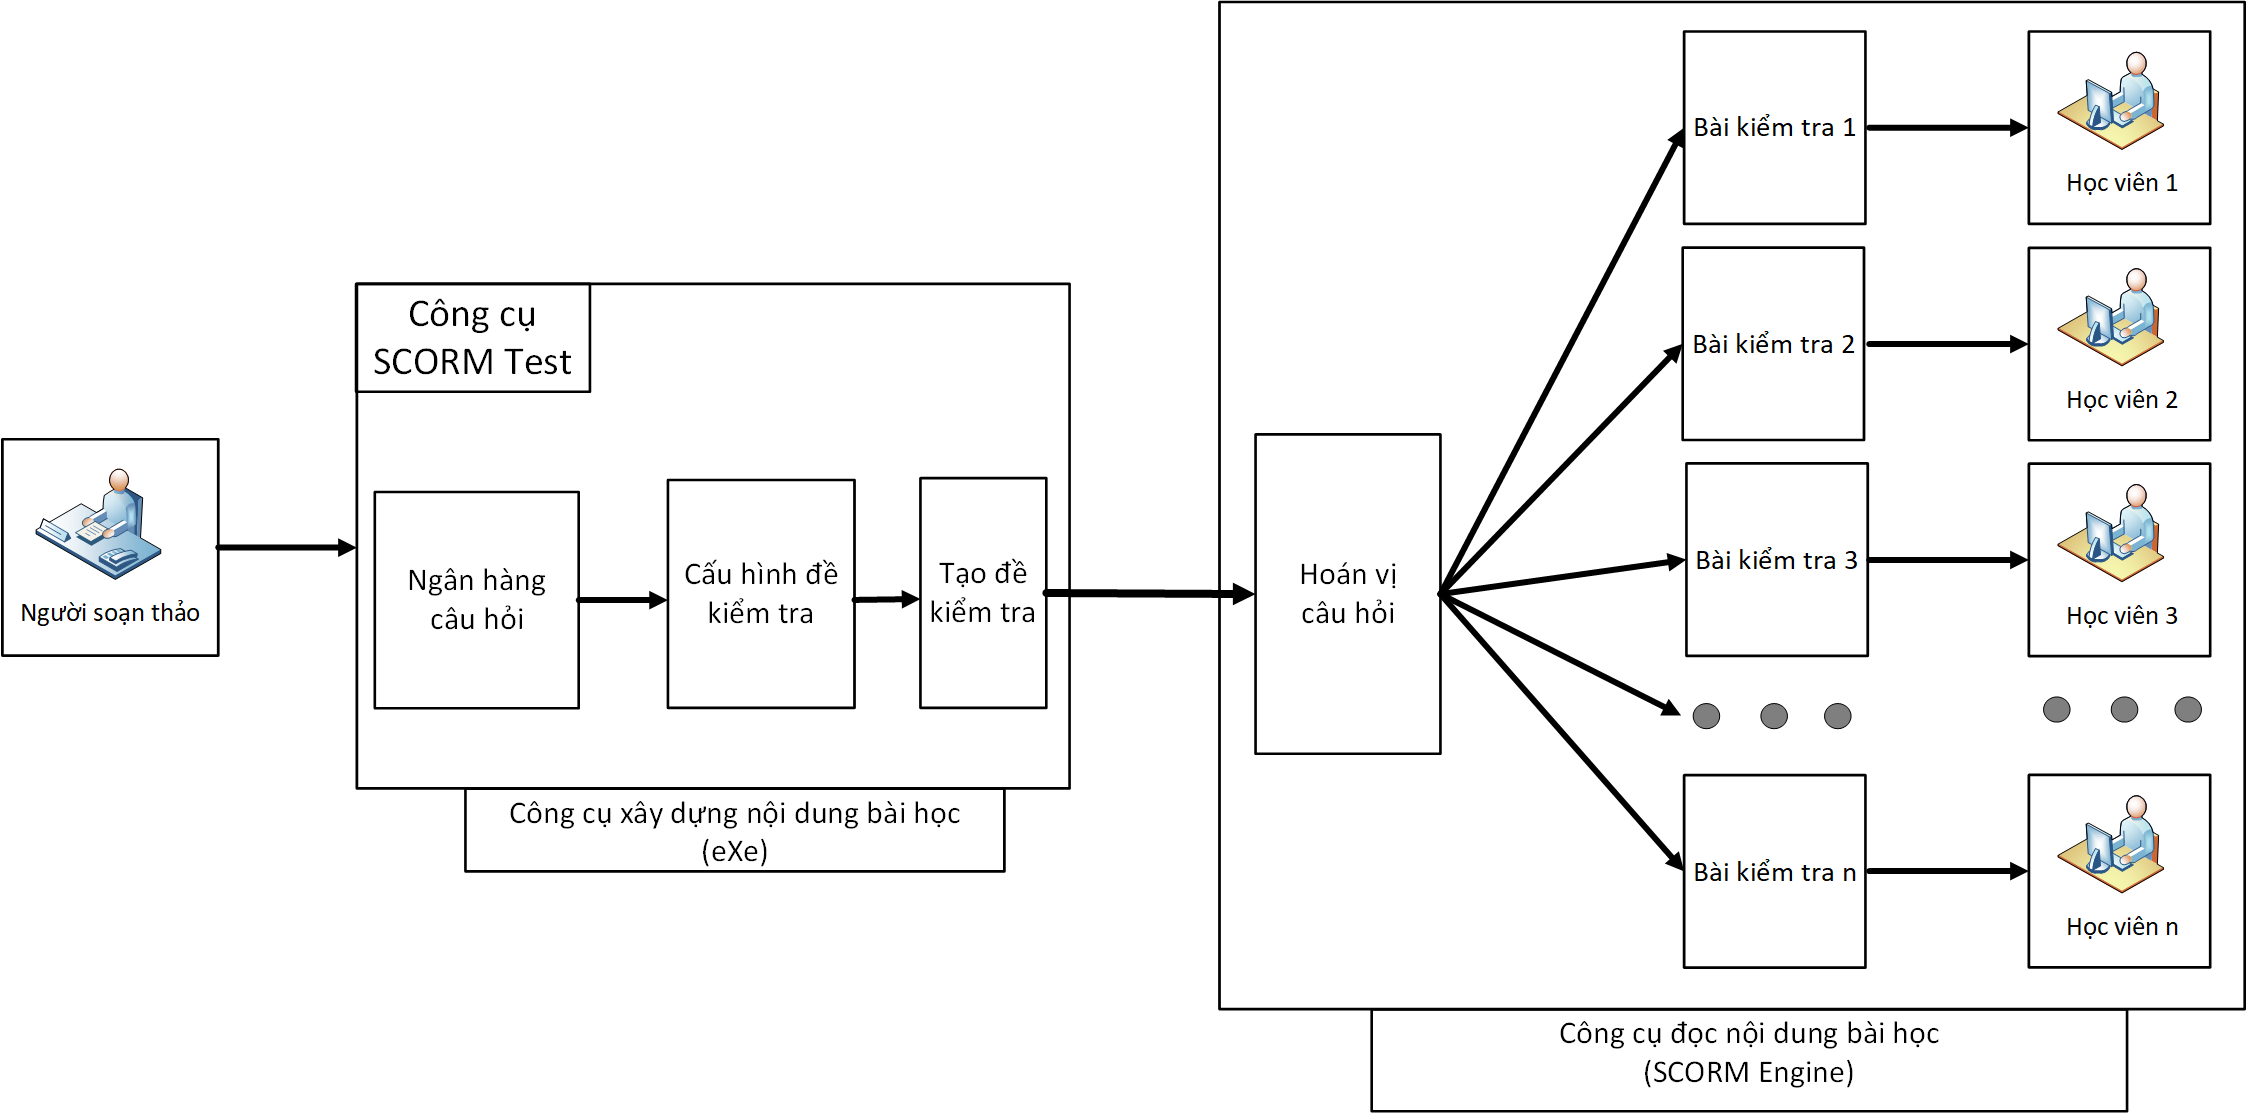
\includegraphics[width=16cm]{Chapter1/Pictures/picture15.png}
		\end{center}
		\caption{Công cụ kiểm tra SCORM Test}
		\label{refpicture14}
	\end{figure}
\end{center}
	
	Hình 1.5 mô tả quá trình sử dụng công cụ SCORM Test. Người soạn thảo sẽ sử dụng công cụ SCORM Test trên eXe, từ ngân hàng đề thi ban đầu, người soạn thảo sẽ tiến hành cấu hình đề thi, chọn ra những câu hỏi theo ý muốn và tạo đề kiểm tra. Sau đó bộ hoán vị câu hỏi bên phía SCORM Engine sẽ đọc bài kiểm tra này và sinh ra những đề kiểm tra tương ứng cho mỗi học viên, thứ tự các câu hỏi cũng như các câu trả lời đều khác nhau đối với mỗi học viên. Điều này sẽ giúp cải thiện chất lượng trong một buổi kiểm tra, các học viên sẽ làm những đề kiểm tra khác nhau và tránh được tình trạng gian lận.

\section{Cấu trúc của báo cáo Luận Văn Tốt Nghiệp}

	Hai chức năng mà nhóm phát triển là thêm các thông tin điều khiển có điều kiện cho các bài học và thiết kế một công cụ giúp tổng hợp câu hỏi và sinh đề kiểm tra. Để hiện thực hai chức năng này, kiến trúc hệ thống của E-Learning, các mô tả của chuẩn SCORM, những kiến thức, công nghệ dùng để phát triển công cụ eXe và kiến trúc hệ thống của eXe đều được tìm hiểu và trình bày ở chương 2. Chương 3 sẽ trình bày chi tiết về cách tích hợp chức năng điều khiển có điều kiện vào công cụ eXe, đưa ra các khái niệm về điều khiển có điều kiện, các mục tiêu, khó khăn và thách thức trong quá trình thực hiện cũng như cơ chế và cách hiện thực chức năng. Nhu cầu cần kiểm tra kiến thức sau bài học, các nhược điểm của bài kiểm tra được tích hợp sẵn trong công cụ eXe cũng như cách thiết kế công cụ để tổng hợp câu hỏi và sinh đề kiểm tra sẽ được trình bày trong chương 4. Chương 5 sẽ trình bày về kiểm thử phần mềm sau khi hiện thực hai chức năng, bao gồm chiến lược kiểm thử, các khó khăn và thách thức trong quá trình kiểm thử cũng như các hướng giải quyết cho các thách thức này và cuối cùng là một số mẫu kiểm tra nhóm đã hiện thực. Phần cuối cùng, chương 6 sẽ đưa ra kết luận về quá trình, tiến độ cũng như kết quả thực hiện đề tài, cuối cùng là các hướng phát triển tiếp theo có thể thực hiện trong tương lai.




\chapter{CÁC KIẾN THỨC NỀN TẢNG}

	\fontsize{12pt}{7pt}\selectfont
	\noindent\textit{Chương này sẽ giới thiệu một cách tổng quan về E-Learning, chuẩn SCORM và công cụ đọc nội dung theo chuẩn SCORM. Tiếp theo sẽ trình bày công cụ eXe Learning được lựa chọn để phát triển, bao gồm các công nghệ được sử dụng, kiến trúc hệ thống cũng như kiến trúc phần mềm của nó. Cuối cùng sẽ giới thiệu công cụ kiểm thử tự động được dùng để kiểm thử các chức năng của eXe.}


\section{Giới thiệu về E-Learning}
	Cùng với sự phát triển lớn mạnh của công nghệ thông tin, việc dạy và học truyền thống cũng đã có những thay đổi lớn nhờ vào việc ứng dụng công nghệ E-Learning vào trong việc dạy và học. E-Learning là một công nghệ mới, với nhiều ưu điểm so với học tập truyền thống. Trong những năm 2000, các doanh nghiệp lớn trên thế giới đã ứng dụng E-Learning để đào tạo nhân viên của họ, E-Learning giúp tạo một hệ thống thông tin tương tác cao giữa các nhân viên, giúp họ dễ dàng trao đổi để nâng cao nghiệp vụ của mình. Ngày nay, E-Learning được ứng dụng rộng rãi trong hệ thống đào tạo tại các trường đại học và các trung tâm đào tạo lớn.\\

	E-Learning(Giáo dục trực tuyến) là một hình thức học tập thông qua mạng Internet dưới dạng các khóa học và được quản lý bởi các hệ thống quản lý học tập, nhằm đảm bảo sự tương tác, hợp tác và đáp ứng nhu cầu học mọi lúc, mọi nơi của người học. Khác với các phương pháp học tập truyền thống, người học sẽ được truyền tải kiến thức thông qua nội dung được các giảng viên xây dựng, biên soạn sẵn. Các nội dung truyền đạt kiến thức được thể hiện bằng nhiều hình thức khác nhau như video, hình ảnh, bài tập vận dụng,... Bên cạnh đó E-Learning cũng cung cấp một môi trường học tập tương tác cao như diễn đàn, nhóm trao đổi hay các bài tập đánh giá,...\\

	Mở rộng ra, các cá nhân hay tổ chức đều có thể tự lập ra một trường học trực tuyến(E-School) để nhận đào tạo học viên, đóng học phí, có các bài kiểm tra và được cấp chứng nhận sau khi hoàn thành khóa học như một trường học truyền thống. Một số trường học trực tuyến phổ biến hiện nay có số lượng học viên lớn như Udemy, Edumall, hocmai.vn,... Phần lớn các trường đại học trên thế giới nói chung hay Việt Nam nói riêng đều có hệ thống E-Learning để phục vụ tốt hơn cho việc dạy và học của giảng viên và sinh viên. E-Learning đã thay đổi hoàn toàn phương pháp học tập truyền thống, phần sau đây sẽ trình bày một số ưu điểm và nhược điểm của việc sử dụng hệ thống E-Learning trong giáo dục.

\newpage

\subsection{Ưu điểm của E-Learning so với học tập truyền thống}

	Mặc dù không thể thay thế hoàn toàn phương pháp học tập truyền thống nhưng E-Learning phần nào cũng đã khắc phục, củng cố những hạn chế của phương pháp học tập truyền thống. Một số ưu điểm của E-Learning có thể kể đến như:

	\begin{itemize}
		
		\item \textbf{Tiết kiệm chi phi đào tạo:} Nội dung của bài giảng E-Learning có thể sử dụng cho nhiều khóa học khác nhau nên có thể tiết kiệm được từ 40\% đến 60\% chi phí đào tạo so với hình thức đào tạo truyền thống.
	
		\item \textbf{Độ linh hoạt cao:} Học viên sẽ không bị giới hạn bởi không gian và thời gian. Chỉ cần có một đường truyền Internet là học viên có thể tiến hành học ở bất cứ đâu và bất cứ lúc nào.
	
		\item \textbf{Tính tương tác cao:} Sự hỗ trợ mạnh mẽ của các đa phương tiện như hình ảnh, âm thanh, hoạt hình hay các công cụ giả lập,... giúp cho bài học sinh động hơn, cuốn hút hơn và cũng dễ hiểu hơn.
	
		\item \textbf{Tính chủ động cao:} E-Learning chủ yếu dựa trên tính chủ động của người học. Thậm chí có một số quan điểm xem E-Learning là việc ứng dụng công nghệ để hỗ trợ cho việc tự học. Người dùng ngoài việc chủ động chọn khóa học, nội dung và thời gian, còn có thể tự đánh giá khả năng của mình qua các bài kiểm tra của nội dung đó để bảo đảm có được lượng kiến thức cần thiết trước khi chuyển sang nội dung khác. Người học cũng có thể theo dõi tiến độ học tập của mình nhờ vào những công cụ quản lý của hệ thống E-Learning.
	
		\item \textbf{Tính mở rộng cao:} Với sự giúp đỡ của các trình soạn thảo nội dung hiện nay thì việc thiết kế một bài giảng có các nội dung phong phú, bài tập đa dạng,... là hoàn toàn có thể thực hiện được.
	
	\end{itemize}


\subsection{Nhược điểm của E-Learning}
	
	Những hạn chế của phương pháp học tập trực tuyến(E-Learning) so với phương pháp học tập truyền thống có thể kể đến như sau:

	\begin{itemize}
		
		\item \textbf{Giảm khả năng giao tiếp:} Dù nội dung bài học có sinh động, phong phú đến đâu cũng sẽ không tốt bằng sự chỉ bảo tận tình của giảng viên. Việc chỉ áp dụng học trực tuyến sẽ khiến người học khó kết giao bạn bè, đồng thời cũng hạn chế sự giao tiếp với bên ngoài.
	
		\item \textbf{Không tạo được môi trường học tập tích cực chủ động:} Người học chủ yếu học được kiến thức nhưng không học được cách vận dụng những kiến thức đó một cách thực tế. Ngoài ra người học còn bị hạn chế phát triển một số kỹ năng đòi hỏi tính tương tác cộng đồng cao như kỹ năng làm việc nhóm, kỹ năng thuyết trình,...
	
		\item \textbf{Dễ gây mất tập trung:} Việc ngồi hàng giờ trước máy tính để tập trung vào bài học rất dễ khiến người học bị phân tâm, dẫn đến hiệu quả học tập không cao.
		
	\end{itemize}

\newpage

\subsection{Kiến trúc của hệ thống E-Learning}

\subsubsection{Kiến trúc nền của hệ thống}

	Mô hình kiến trúc nền do tổ chức UKeU(UK eUniversities Worldwide) đưa ra vào năm 2002[1]. UKeU là một tổ chức được thành lập để cộng tác cùng các trường đại học tại Anh, nhằm thúc đẩy việc ứng dụng E-Learning trong trường học. Mô hình kiến trúc này khá phù hợp với các yêu cầu của hệ thống E-Learning và đã được áp dụng ở nhiều hệ E-Learning tiêu biểu trên thế giới. Nó được đánh giá là một mô hình kiến trúc đảm bảo tính mở, linh hoạt, dễ sử dụng và thuận lợi cho việc phát triển hệ thống sau này. Mô hình này cũng đảm bảo được sự kết hợp của hệ thống quản lý giáo trình, quản lý đào tạo và giao diện tương tác của các tác nhân với hệ thống. \\

\begin{center}
	\begin{figure}[htp]
		\begin{center}
			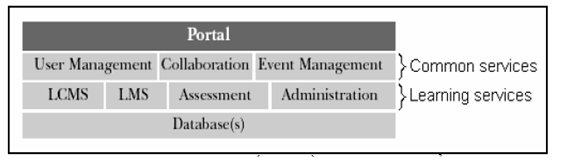
\includegraphics[width=15cm]{Chapter2/Pictures/picture21.png}
		\end{center}
		\caption{Mô hình kiến trúc nền tảng của hệ thống E-Learning}
		\label{refpicture21}
	\end{figure}
\end{center}

	Hình 2.1 mô tả mô hình kiến trúc nền của hệ thống E-Learning gồm 4 tầng liên quan với nhau là tầng cổng (Portal), tầng dịch vụ chung (Common Services), tầng dịch vụ đào tạo (Learning services) và tầng cơ sở dữ liệu (Databases). Tầng Portal chứa những giao tiếp với hệ thống. Tầng Common services chứa những dịch vụ dùng chung cho toàn hệ thống và Tầng Databases chứa cơ sở dữ liệu. Các tầng trên đều là những tầng dịch vụ thường thấy ở bất kì hệ thống nào. Phần sau đây sẽ trình bày điểm riêng của hệ thống E-Learning với các hệ thống khác, nằm ở tầng Learning Services. Tầng Learning Services gồm có:
	\begin{itemize}
		
		\item \textbf{Hệ quản trị nội dung LCMS (Learning Content Management System):} là một ứng dụng phần mềm cho phép tạo nội dung, lưu trữ, quản lý và xuất bản những nội dung đào tạo để phân phối qua mạng, LCMS cần cung cấp những khả năng mềm dẻo nhất cho việc soạn bài giảng, quản lý bài giảng,... Ngày nay có rất nhiều ứng dụng bên thứ 3 cho phép làm việc này, một số công cụ còn được thương mại hóa với độ ổn định cao.
	
		\item \textbf{Hệ quản trị đào tạo LMS (Learning Management System):} là phần mềm tự động hóa việc quản lý các sự kiện đào tạo. LMS ghi nhận các thao tác của người dùng, tạo các khoá học, phân cấp khóa học theo các danh mục khóa học và cung cấp các bản thông báo cho việc quản lý. Một hệ LMS được thiết kế để có thể kiểm soát các khoá học từ nhiều nguồn xuất bản và nhiều nhà cung cấp. Một số LMS phổ biến hiện nay và được open-source như Moodle, Sakai,...
	
		\item \textbf{Hệ thống đánh giá:} là hệ thống đánh giá khả năng của học viên đối với khóa học, sử dụng những câu hỏi kiểm tra hay các bài tổng kết, bài tập lớn,... Từ chỗ đánh giá việc học của học viên, nó cho phép chọn những bài giảng phù hợp nhất cho học viên trong một khoá học cụ thể.
	
		\item \textbf{Hệ thống quản lý:} cho phép người quản lý bao quát được tất cả các học viên, giảng viên và những người dùng của hệ thống, cho phép tổng hợp, đánh giá dễ dàng, liên tục các dữ liệu liên quan. 	
		
	\end{itemize}

	Trong những hệ thống trình bày trong tầng Learning Services thì có 2 bộ phận quan trọng nhất đó là LCMS và LMS, hai bộ phận này đảm nhận vai trò tạo nội dung và quản lý nội dung trên các hệ thống E-Learning hiện tại. Phần tiếp theo sẽ trình bày về mối quan hệ giữa 2 đơn vị này.\\

\subsubsection{Mối quan hệ LCMS và LMS}

	LCMS và LMS là khác nhau nhưng chúng phối hợp với nhau để mang lại hiệu quả hoạt động cho hệ thống E-Learning. Khi được kết hợp chặt chẽ, thông tin từ hai hệ có thể được trao đổi, chuyển giao cho nhau. Hình vẽ dưới đây thể hiện một mô hình kết hợp giữa hai hệ[2].


\begin{center}
	\begin{figure}[htp]
		\begin{center}
			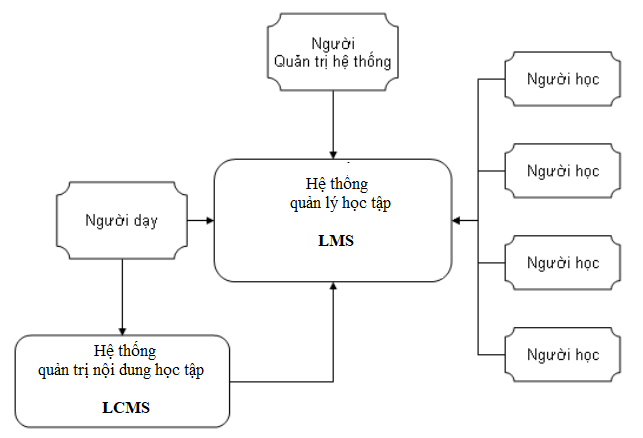
\includegraphics[width=15cm]{Chapter2/Pictures/picture22.png}
		\end{center}
		\caption{Mối quan hệ LMS và LCMS}
		\label{refpicture22}
	\end{figure}
\end{center}

	Hình 2.2 mô tả tổng quan về mối liên hệ giữa 2 đơn vị LCMS và LMS, qua đó người dạy sẽ thông qua hệ thống LCMS để tạo và quản lý nội dung sau đó đưa gói nội dung lên các hệ thống quản lý học tập như Moodle, Sakai,… Người học sẽ được cung cấp tài khoản và đăng nhập vào hệ thống, người quản trị hệ thống sẽ cung cấp các quyền truy cập vào khóa học cho người học.
	
\newpage

\section{Chuẩn SCORM}
	\subsection{Sự ra đời của SCORM}
	
	Khi E-Learning ra đời đã làm phát sinh một số vấn đề liên quan đến việc giao tiếp giữa LCMS và các LMS. Cần có 1 chuẩn đóng gói nội dung để có thể sử dụng với nhiều LMS khác nhau, nhằm giảm chi phí khi có nhu cầu đổi từ LMS này sang một LMS khác tốt hơn. Từ cơ sở để giải quyết vấn đề nêu trên, các tổ chức lớn lần lượt nêu lên các đặc tả để giải quyết như đặc tả về đóng gói nội dung, đặc tả về trao đổi thông tin giữa nội dung và hệ thống đào tạo. Các đặc tả nói trên được phát triển bởi các tổ chức khác nhau và nhằm giải quyết các vấn đề khác nhau trong E-Learning. Mặc dù được chấp nhận như các chuẩn không chính thức trong cộng đồng E-Learning, các đặc tả tồn tại riêng lẻ, không thống nhất và không có quan hệ chặt chẽ với nhau. Để phát triển E-Learning hiệu quả, chi phí thấp cần có một mô hình thống nhất các đặc tả trên lại với nhau. Như vậy, với nhu cầu cần một chuẩn đặc tả chung về việc đóng gói nội dung và giao tiếp giữa LCMS và LMS, từ đó chuẩn SCORM ra đời.

	\subsection{Khái niệm của chuẩn SCORM}
	
	SCORM (Shareable Content Object Reference Model – Mô hình tham chiếu đối tượng nội dung dùng chung) là mô hình tham khảo các chuẩn kỹ thuật, các đặc tả và các hướng dẫn có liên quan được đưa ra bởi các tổ chức khác nhau dùng để đáp ứng các yêu cầu ở mức cao của nội dung học tập và các hệ thống thông qua các từ “ilities” như sau.\\

	\textbf{Môi trường học tập dựa trên chuẩn SCORM có những khả năng sau:}\\

	\begin{itemize}
	
		\item \textit{Tính truy cập được (Accessibility):} Khả năng định vị và truy cập các nội dung giảng dạy từ một nơi ở xa và phân phối nó tới các vị trí khác.
	
		\item \textit{Tính thích ứng được (Adaptability):} Khả năng cung cấp các nội dung giảng dạy phù hợp với yêu cầu của từng cá nhân và tổ chức.
	
		\item \textit{Tính kinh tế (Affordability):} Khả năng tăng hiệu quả và năng suất bằng cách giảm thời gian và chi phí liên quan đến việc phân phối các giảng dạy.
	
		\item \textit{Tính bền vững (Durability):} Khả năng trụ vững với sự phát triển và thay đổi của công nghệ mà không phải thiết kế lại tốn kém, cấu hình lại.
	
		\item \textit{Tính khả chuyển (Interoperability):} Khả năng làm cho các thành phần giảng dạy tại một nơi với một tập công cụ hay platform và sử dụng chúng tại một nơi khác với một tập các công cụ hay platform.
	
		\item \textit{Tính sử dụng lại (Reusability):} Khả năng mềm dẻo trong việc kết hợp các thành phần giảng dạy trong nhiều ứng dụng và nhiều ngữ cảnh khác nhau.
	
	\end{itemize}


	Nhờ những khả năng trên của chuẩn SCORM mà hiện nay SCORM được sử dụng nhiều nhất khi xây dựng một bài giảng E-Learning.
	
\newpage

	\subsection{Các phiên bản của SCORM}
	
	Các phiên bản của SCORM ngày càng được hoàn thiện để thực hiện đầy đủ các yêu cầu về các tính năng. Các phiên bản SCORM đã ra đời là: SCORM 1.1, SCORM 1.2, SCORM 1.3 hay còn gọi là chuẩn SCORM 2004. \\

	Tháng 1/2004, SCORM 2004 được công bố và là phiên bản ổn định, ADL hứa hẹn rằng trong tương lai gần, sẽ không có những thay đổi lớn đối với các chuẩn hiện có. ADL chỉ tập trung vào việc mở rộng phạm vi của SCORM và bổ sung các phần mới vào tài liệu hiện tại. Sẽ có những cập nhật trong tương lai song nó sẽ không làm đảo lộn mọi thứ, chắc chắn nội dung tương thích với SCORM 2004 vẫn có thể sử dụng lại được. Hệ thống tương thích với SCORM 2004 sẽ không cần phải sửa lại toàn bộ theo phiên bản tiếp theo của SCORM. \\

	SCORM 2004 được xem là nền móng vững chắc cho sự phát triển của các nội dung và các ứng dụng liên quan tới nó.\\


	\subsection{Tổ chức đặc tả của chuẩn SCORM}
	
	SCORM là một tập hợp những chuẩn đặc tả, được tổ chức thành bốn cuốn tài liệu: SCORM Overview, SCORM CAM (SCORM Content Aggregation Model), SCORM RTE (SCORM Run-Time Enviroment) và SCORM Sequencing and Navigation[3].\\


	\textbf{a. SCORM Overview:}\\
	Cuốn sách này trình bày mục tiêu và lịch sử phát triển của hệ thống ADL và SCORM. Nó cũng là tài liệu tổng quan hướng dẫn sử dụng những cuốn sách khác của SCORM.\\
	
	\vspace{0.5cm}
	
	\textbf{b. SCORM CAM:}\\
	Cuốn sách này trình bày những nội dung như sau:
	\begin{itemize}
		\item \textit{Định nghĩa các thành phần sử dụng trong một bài học.}
		\item \textit{Đóng gói các thành phần.}
		\item \textit{Mô tả các thành phần để có thể tìm kiếm và khai phá.}
		\item \textit{Định nghĩa các luật sắp xếp cho các thành phần trong bài học.}									
	\end{itemize}


	Để thực hiện nội dung đó, SCORM CAM định nghĩa nhiệm vụ và đưa ra yêu cầu đối với việc xây dựng những tập hợp nội dung (khóa học, bài học, module,…) đồng thời đề xuất cấu trúc và tổ chức cho những tập hợp nội dung đó. SCORM CAM cũng đề cập đến những quy tắc cần tuân thủ khi tạo gói tin nội dung, cách sử dụng metadata để mô tả các thành phần trong gói nội dung nhằm phục vụ cho việc tìm kiếm, lưu trữ và sử dụng lại.\\
	\vspace{0.5cm} 
	
	\textbf{c. SCORM RTE:}\\	
	Mô tả những yêu cầu của LMS để quản lý nôi trường thực thi (xử lý thể hiện nội dung, thông tin giữa nội dung và LMS, phần tử mô hình dữ liệu chuẩn được sử dụng để chuyển thông tin đến người học).\\
	
	\vspace{0.5cm}
	
	\textbf{d. SCORM Sequencing and Navigation:}\\	
	Mô tả các thông tin điều hướng nội dung trong bài học. Hướng người học theo một kịch bản mà người biên soạn muốn[3]. Cung cấp một số mô hình điều hướng thường sử dụng như: “Linear”, “No Sequencing”, “Constraint Choice”,...	
	
	

\newpage

\subsection{Gói nội dung (Content Package) được đóng gói theo chuẩn SCORM}

	SCORM cung cấp những đặc tả một cách chi tiết về những kỹ thuật cơ bản trong E-Learning như metadata, gói nội dung và xác định cơ chế cho việc giao tiếp với nội dung học tập. Một gói nội dung trong SCORM có thể là một bài học, một khóa học hay một môn học, được đóng gói thành file .zip, sau đó import vào các LMS.\\

	Gói nội dung của SCORM được mô tả như sau:\\

\begin{center}
	\begin{figure}[htp]
		\begin{center}
			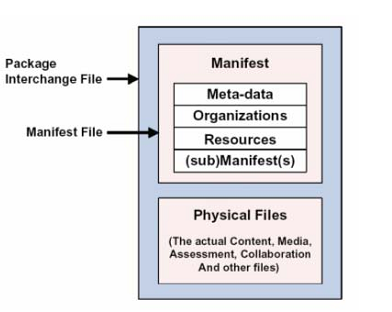
\includegraphics[width=16cm]{Chapter2/Pictures/picture23.png}
		\end{center}
		\caption{Cấu trúc của một đối tượng trong SCORM}
		\label{refpicture23}
	\end{figure}
\end{center}

\newpage

	Các thành phần có trong gói nội dung: \\
	
	\begin{itemize}
	
	\item \textbf{File imsmanifest.xml:} là file XML (imsmanifest.xml) nằm ở mức độ cao nhất đặc tả cho việc đóng gói nội dung. Nó điều hướng cho Hệ thống quản lí việc học (Learning Management System-LMS) xác định các nguồn tài nguyên được sử dụng trong bài học. Ngoài ra file này sẽ cung cấp các thông tin điều hướng nội dung theo chuẩn SCORM. Trong file này sẽ bao gồm những nội dung sau:\\

	\begin{itemize}
		\item \textbf{Meta-data}: Phần này được trình bày đầu tiên trong file imsmanifest.xml, là phần cung cấp thông tin về gói nội dung, tác giả cũng như chuẩn SCORM hỗ trợ.
	
		\item \textbf{Organizations}: Là phần tiếp theo trong file imsmanifest.xml, là thành phần chứa dữ liệu về cấu trúc nội dung trong gói. Cấu trúc này là cách sắp xếp nội dung bài học theo từng chương, từng mục. Các thông tin điều hướng các hoạt động của bài học cũng được trình bày tại đây.
	
		\item \textbf{Resources}: Phần cuối trong file imsmanifest.xml, dùng để chứa các đường dẫn đến các tài nguyên trong bài học.
	\end{itemize}


	\item \textbf{Physical Files:} Bao gồm hai thành phần, thứ nhất là các file hệ thống của SCORM và thứ hai là các file chứa nội dung bài học, các file media phục vụ cho nội dung của bài học, các file này do người biên soạn tạo ra.\\

\end{itemize}
\vspace{0.5cm}
Như vậy việc tạo một gói SCORM bao gồm các công việc:
\begin{itemize}
	\item Tạo 1 thư mục gốc để chứa các file thành phần.
	\item Tạo (copy) các file hệ thống của SCORM vào thư mục gốc.
	\item Tạo (copy) các file của bài học vào thư mục gốc.
	\item Biên tập file imsmanifest.xml cho phù hợp với các file của bài học.
	\item Đóng gói tất cả các file vào một file zip.
\end{itemize}

\subsection{SCORM Engine - Công cụ đọc nội dung theo chuẩn SCORM}
\subsubsection{6.1 Giới thiệu SCORM Cloud}
SCORM Cloud là một Hệ quản trị đào tạo (Learning Management System) trực tuyến. SCORM Cloud cung cấp một môi trường quản lý học tập trực quan, mô hình quản lý học tập này vẫn tuân theo cấu trúc đã đưa ra ở hình 2.2.\\

Với SCORM Cloud, người dạy có thể tạo nội dung học tập hoặc dùng các nội dung đã có upload lên. Những bài học này sẽ được thêm vào thư viện của người dạy, sau đó người dạy có thể theo dõi trạng thái của từng bài học khác nhau thông qua các thông số mà SCORM Cloud cung cấp như số người tham gia vào bài học này, thống kê số người hoàn thành khóa học, thời gian khóa học thường bắt đầu,... Hình 2.4 mô tả một số thông tin người dạy có thể theo dõi của khóa học hiện tại.\\

\vspace{0.5cm}

\begin{center}
	\begin{figure}[htp]
		\begin{center}
			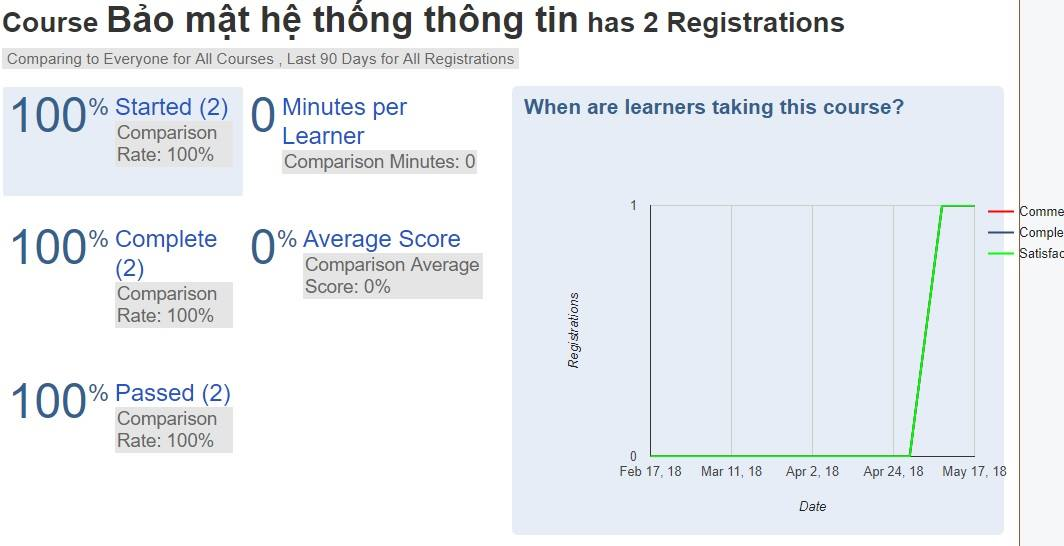
\includegraphics[width=15cm]{Chapter2/Pictures/picture24.jpg}
		\end{center}
		\caption{Thông tin một khóa học trên SCORM Cloud}
		\label{refpicture24}
	\end{figure}
\end{center}
\newpage

\subsubsection{6.2 Ưu điểm của SCORM Cloud so với các LMS khác}
SCORM Cloud hoạt động như là một dịch vụ Web nên không cần phải cài đặt, chỉ cần trình duyệt web là có thể sử dụng được. Với những Hệ quản trị đào tạo mã nguồn mở như Moodle, Sakai,... Người quản lý có thể dễ dàng tùy chỉnh thiết lập của mình, thay đổi source,... tùy vào mục đích sử dụng. Còn SCORM Cloud đã được thường mại hóa, do Rustici Softwares phân phối nên không  thể điều chỉnh giao diện quản lý theo ý người sử dụng, nhưng bù lại không cần tốn chi phí cài đặt server, tính ổn định của nó rất cao và hỗ trợ quản lý khóa học cực kỳ hiệu quả. Chỉ cần đăng ký tài khoản là có thể sử dụng các dịch vụ của SCORM Cloud. Hình 2.5 giới thiệu giao diện của người dùng trên SCORM Cloud.\\

\begin{center}
	\begin{figure}[htp]
		\begin{center}
			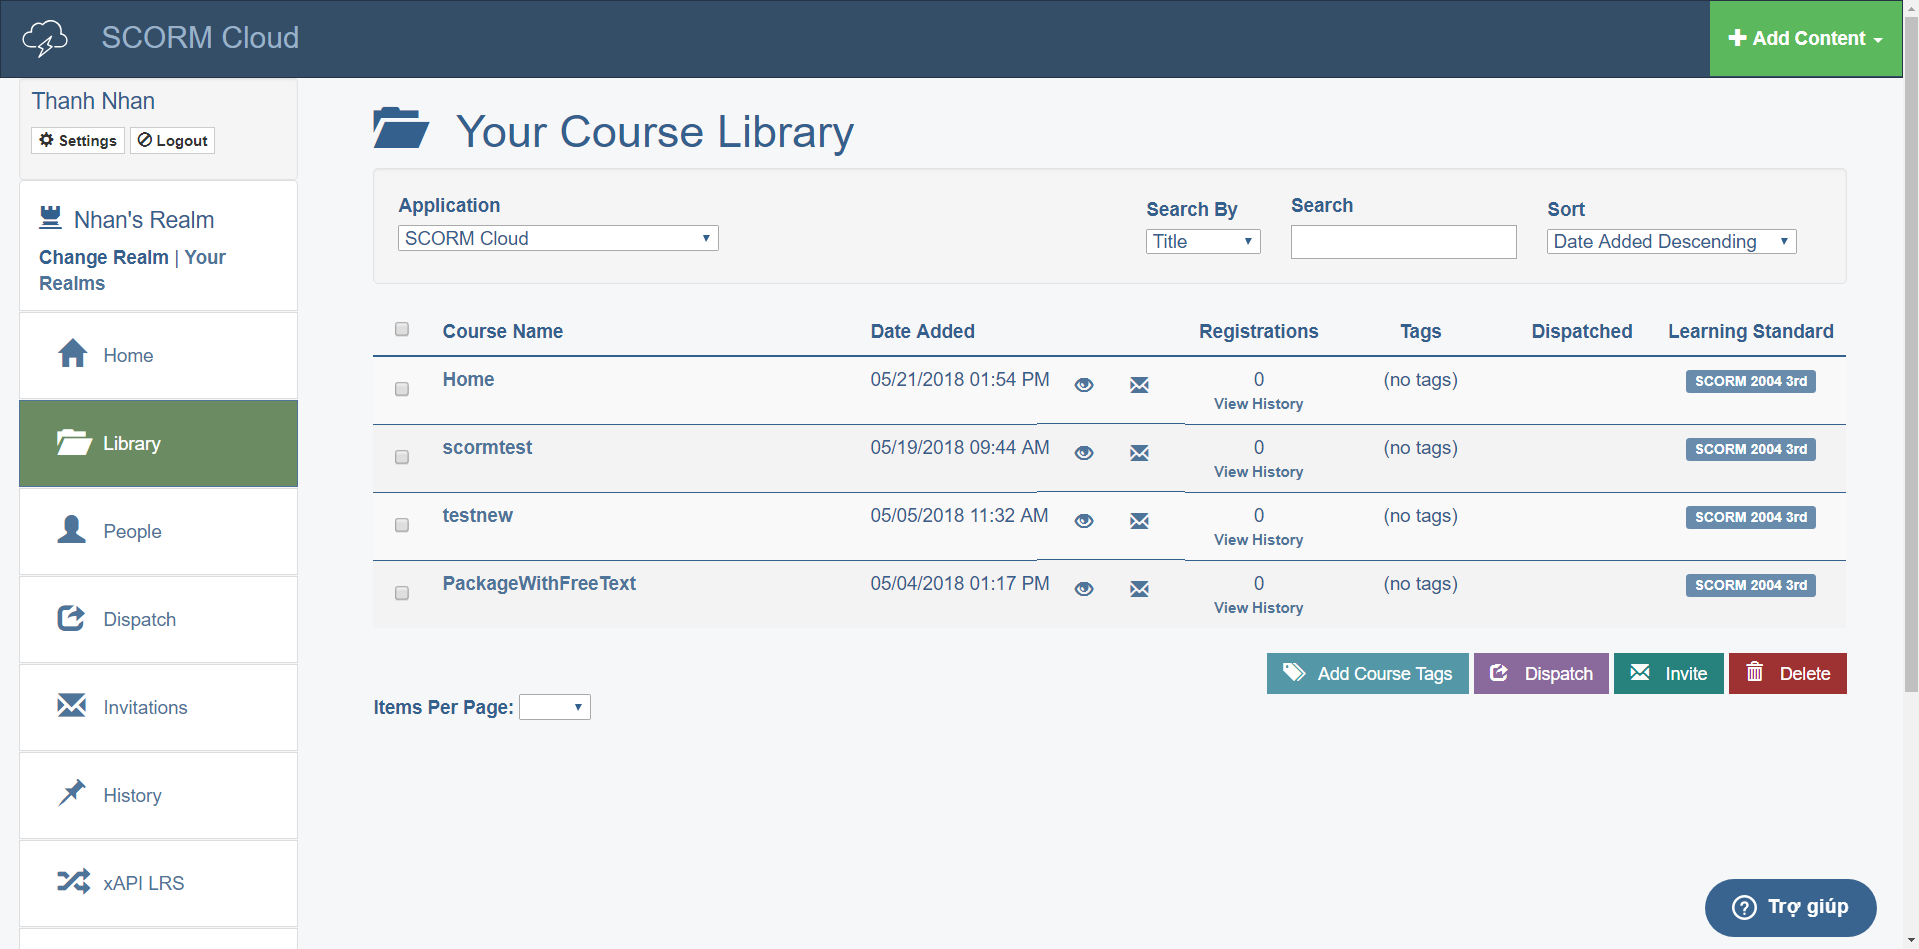
\includegraphics[width=17cm]{Chapter2/Pictures/picture25.png}
		\end{center}
		\caption{Giao diện người dùng trên SCORM Cloud}
		\label{refpicture25}
	\end{figure}
\end{center}


SCORM Cloud hỗ trợ chuẩn SCORM rất tốt, có thể nói đây là SCORM Engine mạnh nhất hiện nay. Nếu như Moodle hay Sakai bị hạn chế một số tính năng của chuẩn SCORM,  như Moodle không hỗ trợ những đặc tả Sequencing(điều hướng) của chuẩn SCORM 2004,  thì SCORM Cloud hỗ trợ đầy đủ các tính năng cho tất cả các phiên bản SCORM khác nhau, từ SCORM 1.2 đến phiên bản mới nhất SCORM 2004 phiên bản thứ 3.\\

Hình 2.6 mô tả cách sử dụng SCORM Cloud, đầu tiên người soạn thảo dùng eXe để biên soạn nội dung bài giảng, đóng gói bài giảng bằng chuẩn SCORM 2004, sau đó upload lên SCORM Cloud để nhiều học viên cùng tham gia vào bài học này.\\


\begin{center}
	\begin{figure}[htp]
		\begin{center}
			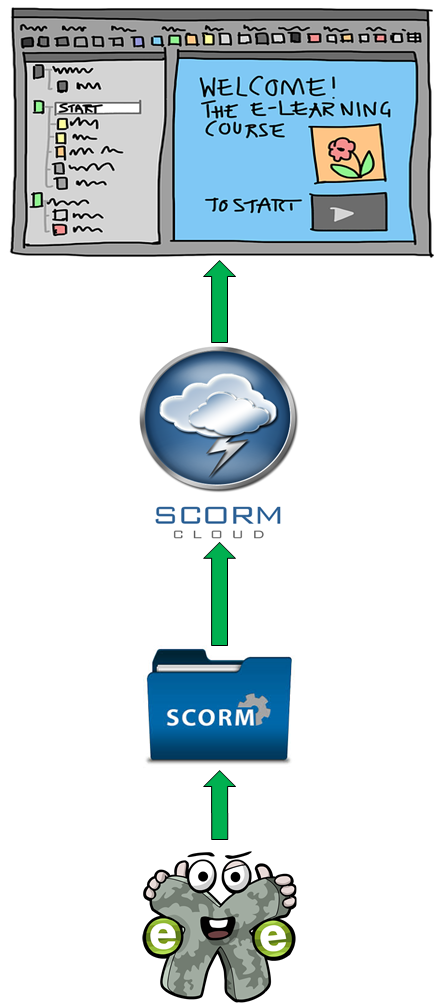
\includegraphics[width=8cm]{Chapter2/Pictures/picture26.png}
		\end{center}
		\caption{Cách sử dụng SCORM Cloud}
		\label{refpicture26}
	\end{figure}
\end{center}

\section{Công cụ eXe Learning}

\subsection{Sơ lược về hệ thống eXe Learning}
\subsubsection{1.1 Lịch sử ra đời của eXe Learning}
eXe Learning là một dự án mã nguồn mở, được tài trợ bởi chính phủ New Zealand và hai trường đại học tại New Zealand là University of Auckland và Auckland University of Technology. Dự án được bắt đầu phát triển vào năm 2007 nhưng không được nhiều thành công như mong đợi. Vào năm 2010, viện đại học INTEF (Tây Ban Nha) quyết định khởi động lại dự án với cái tên mới là “The new eXe Learning” nhưng vẫn giữ các mục tiêu ban đầu là “Free and open source”, nó là phiên bản của eXe Learning hiện tại. Phiên bản hiện tại là phiên bản 2.1.3 được phát hành vào năm 2015. Hiện tại, eXe Learning đã có một cộng đồng người dùng rộng lớn, thường xuyên đóng góp ý kiến trên diễn đàn và hệ thống hứa hẹn sẽ được hỗ trợ lâu dài.\\

\subsubsection{1.2 Giới thiệu phần mềm eXe Learning}
eXe Learning là một ứng dụng trên web, tuy nhiên khi sử dụng, máy tính không cần phải kết nối với Internet do hệ thống vận hành trên localhost server khi cài đặt, việc này sẽ giúp tiết kiệm chi phí vì không cần phải cài đặt server. Vì là ứng dụng trên web nên hệ thống có thể cài đặt trên nhiều hệ điều hành khác nhau.\\

\vspace{1cm}

\begin{center}
	\begin{figure}[htp]
		\begin{center}
			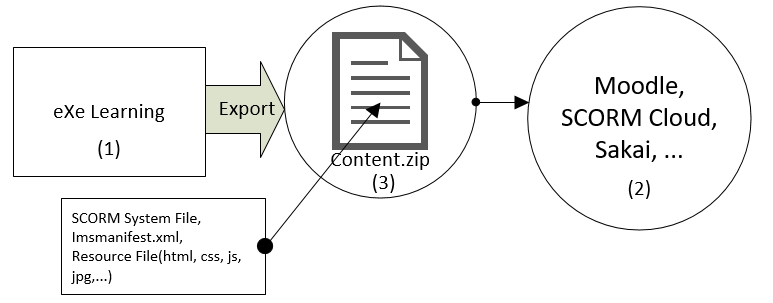
\includegraphics[width=16cm]{Chapter2/Pictures/picture27.png}
		\end{center}
		\caption{Mối quan hệ giữa hệ thống eXe Learning và LMS}
		\label{refpicture27}
	\end{figure}
\end{center}

\newpage

Hình 2.7 là tổng quan về mối quan hệ giữa hệ thống eXe Learning và LMS. (1) là công cụ thiết kế, ở đây cụ thể là eXe Learning. Người dùng sẽ sử dụng công cụ thiết kế để soạn thảo và đóng gói thành sản phẩm (3). Các sản phẩm này sẽ được upload lên các LMS để sử dụng. (2) là một số LMS thông dụng hiện nay. LMS sẽ cung cấp một công cụ gọi là SCORM Engine để đọc và xử lý thông tin trong file nội dung đã được đóng gói.\\

eXe (eLearning XHTML editor) là một công cụ với mục đích dùng để xây dựng nội dung đào tạo trực tuyến. eXe Learning cung cấp một môi trường soạn thảo bài giảng trực quan, hình 2.8 là giao diện tương tác của công cụ gồm có 3 Panel chính, Outline Panel là vùng thiết kế cấu trúc bài học, Idevice Panel là vùng lựa chọn các iDevice và Authoring Panel là vùng soạn thảo nội dung bài học. Bắt chước tính năng “wysiwig” (What You See Is What You Get), eXe cho phép người dùng xem nội dung sẽ trông như thế nào khi được xuất bản trực tuyến, hỗ trợ giáo viên tối đa trong việc thiết kế và xuất bản tài liệu học tập mà không cần có kiến thức về HTML, CSS hay XML. \\

\begin{center}
	\begin{figure}[htp]
		\begin{center}
			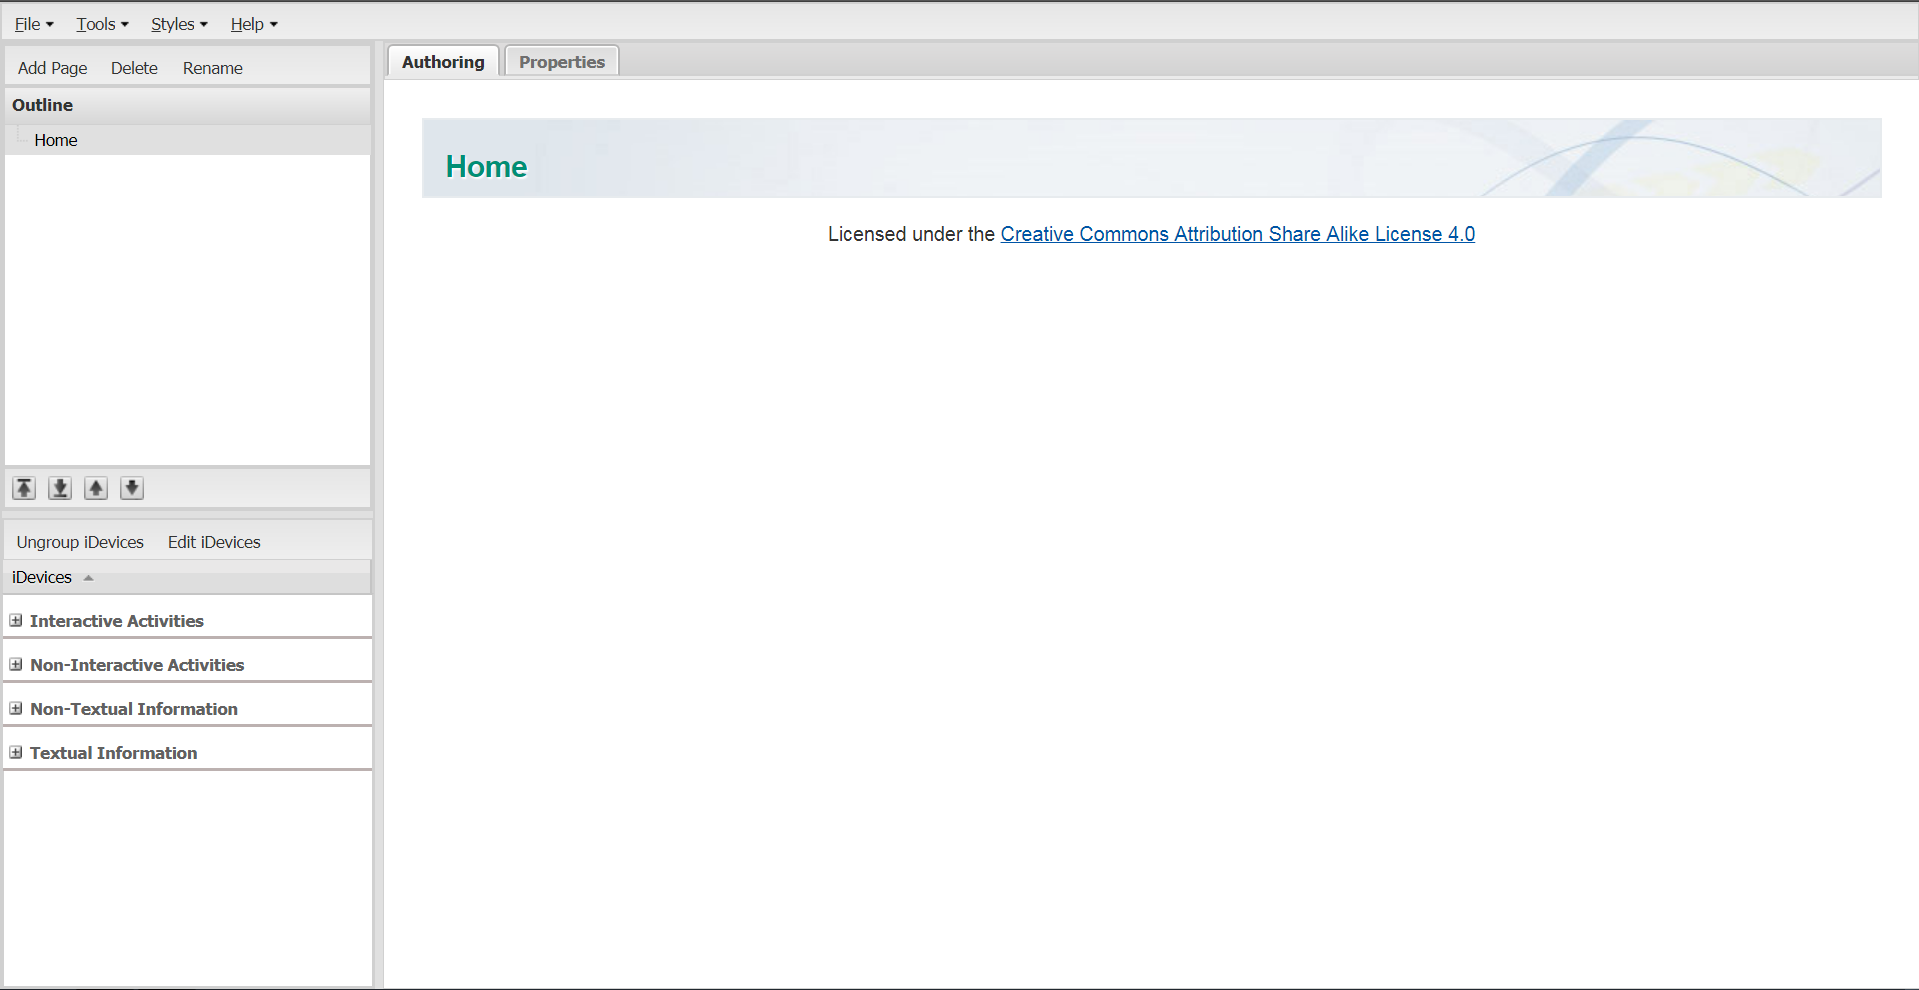
\includegraphics[width=15cm]{Chapter2/Pictures/picture28.png}
		\end{center}
		\caption{Giao diện tương tác của eXe}
		\label{refpicture28}
	\end{figure}
\end{center}	

Nội dung học tập được biên soạn và quản lý theo mô hình cây với các mức level khác nhau do người soạn thảo thiết lập trong Outline Panel. Khi soạn thảo bài học, người biên soạn cần lên một kịch bản rõ ràng, bài giảng sẽ có nhiều Topic, mỗi Topic có nhiều Section, mỗi Section có nhiều Unit được hình thành từ các trang nội dung. Một trang nội dung có thể bao gồm nhiều loại hoạt động khác nhau như câu hỏi trắc nghiệm multi-choice, case study, true-false questions, reading activity,… Các loại hoạt động này được xây dựng sẵn thành các Instruction Device (hay còn gọi là iDevice). iDevice được xem là các module được thiết kế sẵn nhằm mục đích hỗ trợ cho việc soạn thảo bài học. Hình 2.9 mô phỏng cấu trúc nội dung bài học được chia thành nhiều level khác nhau, được thiết kế trong Outline Panel và các iDevice được tích hợp sẵn trong iDevice Panel, các iDevice này được phân ra thành các nhóm như: Interactive Activity, Non-interactive activity, Textual activity,... Việc sử dụng các iDevice này sẽ tùy vào mục đích của người biên soạn.

\newpage

\begin{center}
	\begin{figure}[htp]
		\begin{center}
			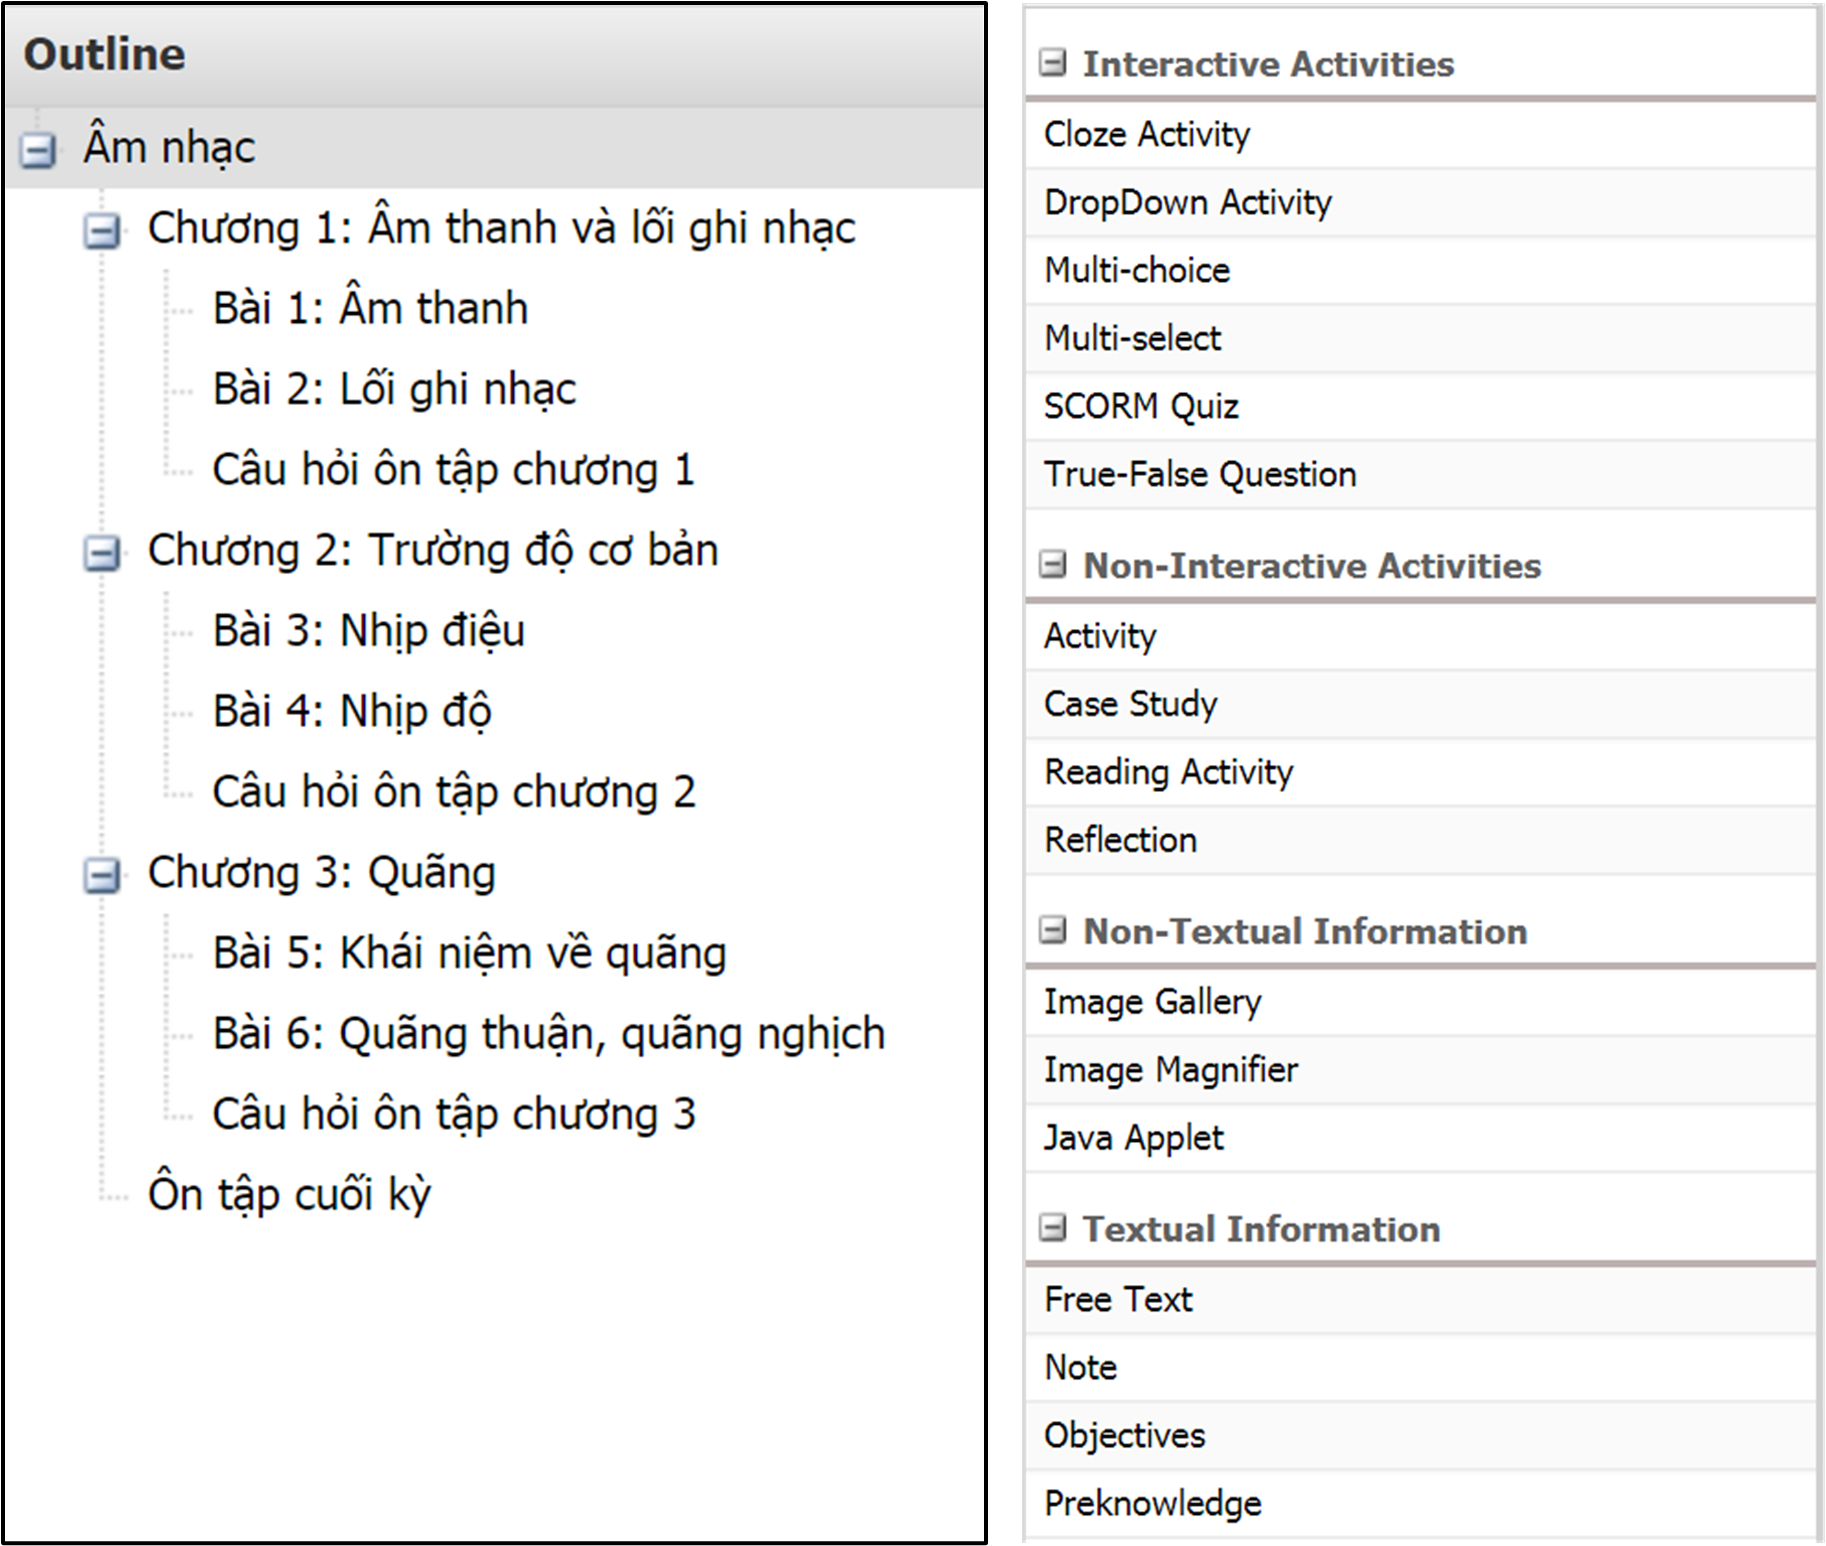
\includegraphics[width=15cm]{Chapter2/Pictures/picture29.png}
		\end{center}
		\caption{Giao diện Outline Panel và iDevice Panel}
		\label{refpicture29}
	\end{figure}
\end{center}

eXe hỗ trợ xuất ra các nội dung soạn thảo thành các định dạng khác nhau như:

\begin{itemize}
	\item Các chuẩn giáo dục: Common Cambridge, SCORM 1.2, SCORM 2004.
	\item Website.
	\item EPUB3.
	\item XLIFF.
\end{itemize}

Các gói nội dung do eXe đóng gói có thể được sử dụng lại, người soạn thảo không cần phải thiết kế lại nội dung khi chuyển từ một LMS này sang một LMS khác. Trong số các chuẩn export trên, được sử dụng phổ biến nhất là chuẩn SCORM có khả năng tương thích với hầu hết các LMS hiện nay. Trong đề tài này LMS được sử dụng để thử nghiệm là SCORM Cloud. Nội dung về SCORM Cloud đã được trình bày ở phần trên.


\subsection{Các công nghệ sử dụng trong hệ thống eXe Learning}
Mô hình Client - Server là một mô hình hết sức phổ biến hiện nay, nó là mô hình mà hầu hết các website hiện nay đang áp dụng. Hệ thống gồm 2 loại phần tử chức năng: server cung cấp 1 số dịch vụ, tài nguyên và đảm nhận vai trò xử lý các yêu cầu và trả kết quả về cho client, client là phần tử sử dụng dịch vụ bằng cách truy xuất đến server tương ứng. Hình 2.10 mô tả sơ lược cách thức hoạt động của mô hình này. Server cần phải đảm bảo có khả năng xử lý nhiều yêu cầu được gửi đến cùng một lúc.\\


\begin{center}
	\begin{figure}[htp]
		\begin{center}
			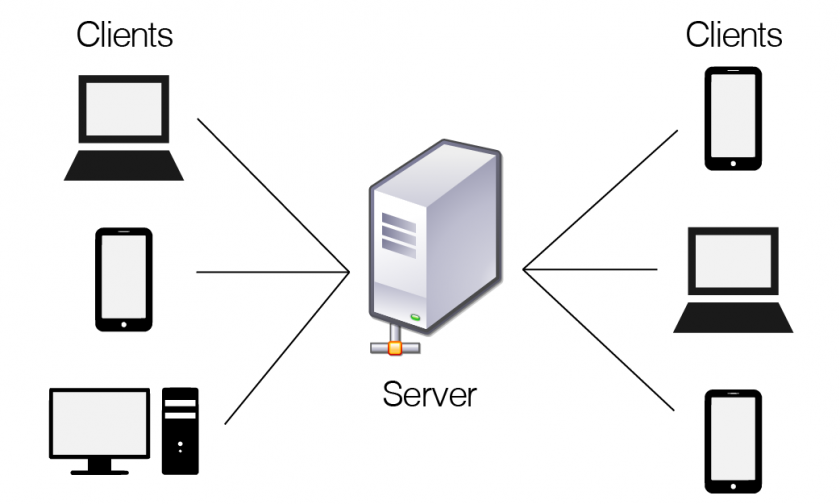
\includegraphics[width=16cm]{Chapter2/Pictures/picture210.png}
		\end{center}
		\caption{Mô hình Client – Server}
		\label{refpicture210}
	\end{figure}
\end{center}

\newpage

\textbf{Server}: Là một máy tính cho phép thực hiện yêu cầu của một hoặc nhiều người dùng từ phía client. Khi có yêu cầu từ phía người dùng, server sẽ chịu trách nhiệm xử lý và trả về kết quả cho người dùng, các kết quả này có thể là một tài nguyên nào đó nằm trên server hay một cái gì đó ví dụ như kết quả của một phép tính. Xét ở một khía cạnh khác thì server có thể được định nghĩa như một máy tính có nhiều người sử dụng vì một server phải xử lý rất nhiều các yêu cầu khác nhau từ nhiều client khác nhau, vì vậy server sẽ hoạt động tốt hơn nếu như có thể xử lý đa nhiệm, tức là các tính năng có khả năng hoạt động một cách độc lập và song song với nhau.\\

\textbf{Client}: Là máy tính chỉ được sử dụng bởi một người dùng, máy client có thể sử dụng các hệ điều hành khác nhau như Windows, Linux, MacOs,... và đóng vai trò tương tác giữa người dùng và server. Bản thân mỗi client được tích hợp nhiều tính năng và khi thông qua kết nối với server, client còn có thể sử dụng thêm những tính năng mà server cung cấp, client chỉ cần nhập các thông tin cần thiết(các tham số đầu vào) và thực hiện gửi yêu cầu lên server, sau khi server xử lý xong sẽ trả về kết quả cho client. Client và server có thể chia sẻ tài nguyên trên máy cho nhau và client được xem là người sử dụng dịch vụ do một hoặc nhiều server cung cấp.\\

eXe Learning hoạt động theo mô hình Client – Server nhưng server là localhost server, có thể xem trình duyệt web là client khi sử dụng. Exe Learning sử dụng ngôn ngữ Python bên phía server và Javascript bên phía Client. Về phía server, eXe sử dụng khung thức Twisted và Nevow để thiết lập localhost server với port mặc định là 55432, còn phía Client sử dụng khung thức ExtJS để thiết kế giao diện. Phần sau đây sẽ giới thiệu các khung thức liên quan này và các ưu nhược điểm của chúng.

\subsubsection{2.1 Khung thức máy chủ: Twisted và Nevow - Khung thức xây dựng ứng dụng mạng}

\begin{enumerate}[a.]
	\item \textit{Twisted - Khung thức mạng}\\
	Twisted là một khung thức xây dựng các ứng dụng mạng có mã nguồn mở, so với các khung thức xây dựng các ứng dụng mạng khác thì Twisted có nhiều ưu điểm nổi trội hơn như sau [4]:
	
	\begin{itemize}
		\item Thứ nhất, nó được hiện thực bằng ngôn ngữ Python, một ngôn ngữ hướng đối tượng rất mạnh, dễ đọc, dễ viết và dễ hiện thực.
		
		\item Thứ hai, vì nó hỗ trợ xử lý bất đồng bộ (Asynchronous) và lập trình hướng sự kiện(event-driven) nên Twisted có thể đảm bảo rằng ứng dụng luôn trong tình trạng có khả năng đáp ứng được nhiều request khác nhau gửi đến cùng 1 lúc, và có khả năng xử lý đồng thời các request này.
		
		\item Thứ ba, Twisted cũng cung cấp gần như đầy đủ các tính năng của nhiều loại server khác nhau tùy vào mục đích sử dụng, các loại server mà Twisted cung cấp như sau:
		\begin{itemize}
			\item \textit{twisted.web}: HTTP clients and servers, HTML templating, and a WSGI server.
			\item \textit{twisted.words}: Clients and servers for IRC, XMPP, and other IM protocols.
			\item \textit{twisted.mail}: IMAPv4, POP3, SMTP clients and servers.
			\item \textit{twisted.positioning}: Tools for communicating with NMEA-compatible GPS receivers.
			\item \textit{twisted.names}: DNS client and tools for making your own DNS servers.
			\item \textit{twisted.trial}: A unit testing khung thức that integrates well with Twisted-based code.																							
		\end{itemize}
		
		\item Cuối cùng là khả năng chia sẻ dữ liệu giữa các hệ thống không sử dụng cùng một protocol, Twisted giúp công việc đó trở nên dễ dàng hơn.
	\end{itemize}
	
	Mô hình eXe chủ yếu chỉ sử dụng module twisted.web để thiết lập local HTTP server.
	
	\item \textit{Nevow - Khung thức ứng dụng mạng}\\
	Nevow là một bộ công cụ xây dựng ứng dụng mạng được viết bằng ngôn ngữ Python do Divmod phát triển. Nevow nhằm mục đích hiện thực một kênh truyền dữ liệu 2 chiều giữa client và server mà không cần tải lại trang, thông qua việc sử dụng đối tượng XMLHttpRequest với các công nghệ như Ajax và DOM. Các dữ liệu máy chủ nhận được từ trình duyệt sẽ được lưu dưới dạng cấu trúc Dictionary của Python, còn dữ liệu mà máy chủ trả về cho trình duyệt được định dạng theo cấu trúc JSON. Nevow hoạt động tốt khi kết hợp cùng với Twisted.[5]\\
	
	\begin{center}
		\begin{figure}[htp]
			\begin{center}
				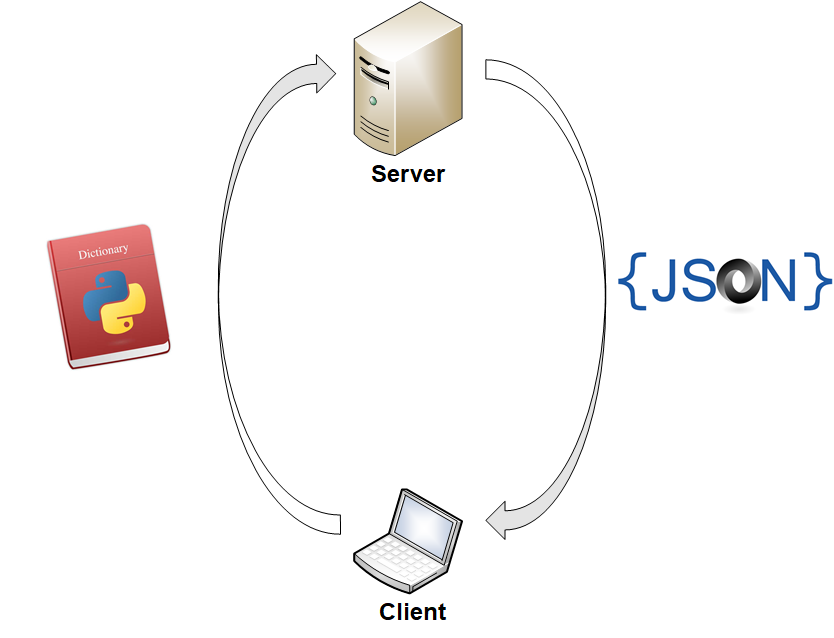
\includegraphics[width=13cm]{Chapter2/Pictures/picture211.png}
			\end{center}
			\caption{Mô phỏng quá trình hoạt động của Nevow}
			\label{refpicture211}
		\end{figure}
	\end{center}
	
	Hình 2.11 mô phỏng quá trình hoạt động của Nevow, các dữ liệu mà máy chủ nhận được từ máy khách (trình duyệt) được lưu dưới dạng cấu trúc Dictionary của Python, sau khi máy chủ xử lý dữ liệu này sẽ gửi về cho máy khách theo định dạng cấu trúc JSON.\\
	
	Tiếp theo sẽ giới thiệu khung thức mà eXe dùng để thiết kế giao diện - ExtJS.

	
\end{enumerate}

\subsubsection{2.2 Khung thức máy khách: Ext JS - Khung thức xây dựng giao diện của Javascript}
Ở phía máy khách, Exe Learning sử dụng ExtJS để thiết kế giao diện[6]. ExtJS là một Khung thức xây dựng giao diện của Javascript được dùng để thiết kế giao diện người dùng rất phong phú và thân thiện, sử dụng các công nghệ như AJAX, DOM và DHTML, do đó các ứng dụng ExtJS có tính tương tác rất cao. Ngoài ra ExtJS còn có khả năng tương tác tốt với Jquery[7]. 

Sau đây là một số đặc điểm của ExtJS:

\begin{itemize}
	
	\item Hỗ trợ đa trình duyệt và điện thoại:
	\begin{itemize}
		\item \textit{Đây là đặc điểm chung của rất nhiều các khung thức lớn có}.
		\item \textit{Được sử dụng để phát triển giao diện trên điện thoại}.
	\end{itemize}
	
	\item Phù hợp với:
	\begin{itemize}
		\item \textit{Những ứng dụng có yêu cầu giao diện đa dạng}.
		\item \textit{Làm ứng dụng trang đơn}.
		\item \textit{Mạnh mẽ với việc hỗ trợ rất nhiều dạng biểu đồ khác nhau, người phát triển không cần sử dụng thêm các công cụ khác để vẽ}.
	\end{itemize}
	
	
	\item Hỗ trợ các mô hình kiến trúc thông dụng:
	\begin{itemize}
		\item \textit{Từ bản ExtJS 4, nó hỗ trợ cả mô hình MVC (Model-View-Controller) và MVVM (Model-View-ViewModel)}.
		\item \textit{Hỗ trợ thao tác trực tiếp với DOM}.
	\end{itemize}
	
	\item Testing:
	\begin{itemize}
		\item \textit{Không hỗ trợ test tự động nhưng có thể thực hiện điều này bằng việc sử dụng thêm các công cụ hỗ trợ test ở level cao hơn}.
		\item \textit{Trong hiện thực đề tài này, nhóm sử dụng Selenium để test chức năng sau khi hiện thực}.
	\end{itemize}
	
	\item Programming:
	\begin{itemize}
		\item \textit{Hỗ trợ mô hình Object-oriented(hướng đối tượng) và Event-driven(hướng sự kiện)}.
	\end{itemize}
	
\end{itemize}

\subsection{Kiến trúc của eXe Learning}
\subsubsection{3.1 Kiến trúc hệ thống eXe Learning}

\paragraph{Mô hình hệ thống – Client Server\\}

Hệ thống eXe Learning được xây dựng là một ứng dụng web (Web Application), thiết kế dựa trên mô hình Client-Server đã được trình bày ở trên, xử lý các yêu cầu gửi tới máy chủ thông qua giao thức HTTP (request và response). Hệ thống sử dụng ngôn ngữ lập trình Python ở phía Server và JavaScript ở phái Client. Khi khởi động, hệ thống thiết lập một localhost server với port 8081 và nhận request từ brower gửi về.[8]

\begin{center}
	\begin{figure}[htp]
		\begin{center}
			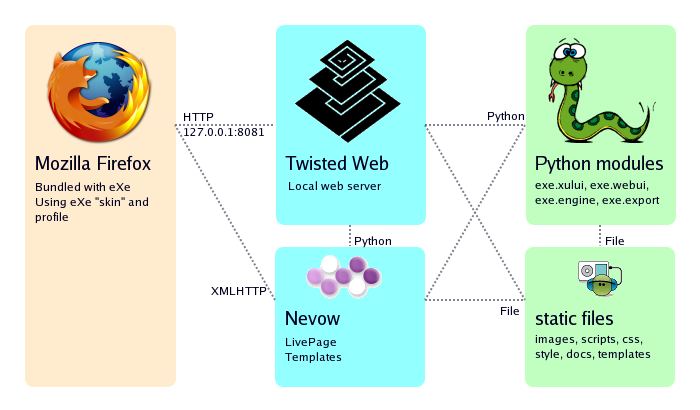
\includegraphics[width=10cm]{Chapter2/Pictures/picture212.png}
		\end{center}
		\caption{Kiến trúc vận hành của eXe}
		\label{refpicture212}
	\end{figure}
\end{center}

Hình 2.12 mô tả cụ thể cách thức hoạt động của hệ thống eXe Learning, mô-đun Twisted Web tạo HTTP localhost server với port cố định 8081 và nhận request. Tiếp theo là việc thiết lập một kênh trao đổi đảm nhận việc xử lý dữ liệu gửi và dữ liệu nhận giữa browser và server. Hệ thống sử dụng khung thức Nevow để đảm nhiệm vai trò trên, xử lý các event và tương tác giữa browser và server. Từ các request gửi về server, hệ thống sẽ phân tích yêu cầu này và gửi yêu cầu đến các module liên quan để xử lý và trả kết quả về cho browser. Các Python modules là các thành phần của phía server nhằm mục đích để xử lý các yêu cầu khác nhau, bao gồm các module giao diện đồ họa, các module đảm nhận việc đóng gói dữ liệu,... Các Static file là các resource file phục vụ cho việc thiết kế giao diện đồ họa. Người dùng sẽ sử dụng trình duyệt web, tạo kết nối tới localhost server.

\subsubsection{3.2 Kiến trúc phần mềm eXe Learning}
Như đã trình bày ở phần trên, phần mềm eXe được viết chủ yếu bằng Python ở phía server và được hiện thực thành nhiều module với các chức năng khác nhau, cụ thể được thể hiện thông qua Class Diagram sau.[9]

\begin{center}
	\begin{figure}[htp]
		\begin{center}
			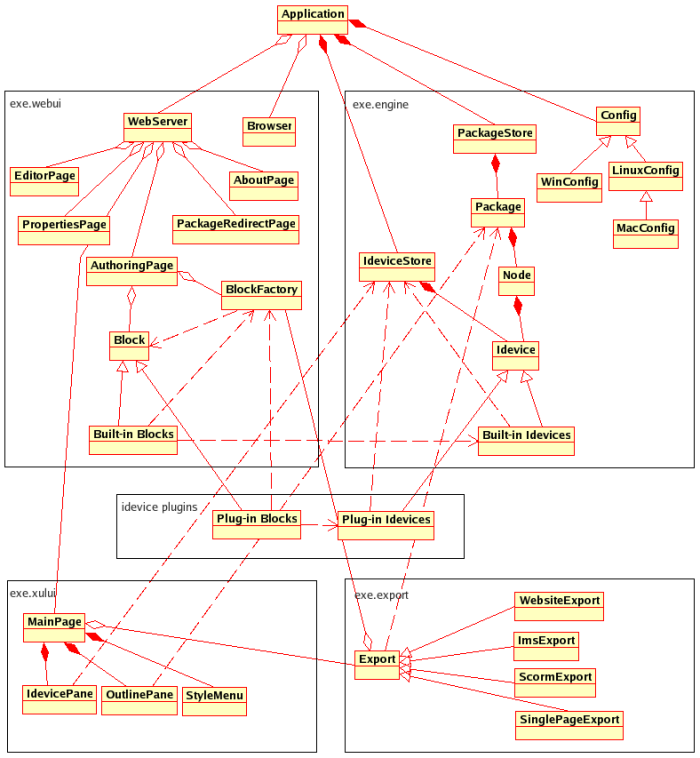
\includegraphics[width=10cm]{Chapter2/Pictures/picture213.png}
		\end{center}
		\caption{Class Diagram của phần mềm eXe}
		\label{refpicture213}
	\end{figure}
\end{center}

\newpage

Hình 2.13 là Class Diagram của eXe, mô tả tổ chức của hệ thống với hàm main của eXe nằm ở Class Application và có các modules khác nhau đảm nhận các chức năng khác nhau [10], cụ thể như sau:

\begin{itemize}
	\item \textbf{Exe.webui}: Gồm 2 Class quan trọng là WebServer và Browser. WebServer với chức năng chính là tạo port trống, sau đó khởi động các dịch vụ của server bằng các phương thức thừa kế từ twisted. Browser với chức năng chính là tìm browser mặc định của hệ điều hành và khởi động với các thiết lập từ Webrowser.
	
	\item \textbf{Exe.engine}: Module này định nghĩa các cấu trúc được sử dụng trong hệ thống như cấu trúc của một package, cấu trúc của một bài học, cấu trúc của một Block, cấu trúc của một iDevice,… Các phương thức xử lý trên chúng cũng như các phương thức xử lý dùng chung đều được định nghĩa trong module này.
	
	\item \textbf{Exe.jsui}: Module này cung cấp các phương thức xử lý request về việc render giao diện và handle các event thao tác trên giao diện. Giao diện eXe sẽ gồm 3 panel chính được mô tả như hình 2.8 và 2.9.
	
	\item \textbf{Exe.Export}: Module này cung cấp các phương thức xử lý yêu cầu đóng gói thành các định dạng khác nhau bao gồm các chuẩn Education Export là SCORM 1.2, SCORM 2004, Common Cartridge, các định dạng website Export là Single Page, Zip File, Self-contain Foder, các định dạng khác là Text File, XLIFF, EPUB3.
	
	\item \textbf{Idevice Plugins}: eXe cung cấp một công cụ tự thiết kế iDevice riêng từ các thành phần có sãn, nhưng các thành phần này bị hạn chế về số lượng nên các iDevice được thiết kế theo công cụ này gần như không có sự khác biệt so với các iDevice có sẵn. Các iDevice này sẽ được lưu trong dữ liệu cục bộ trên máy tính.									
\end{itemize}



\section{Công cụ kiểm thử sản phẩm}

\subsection{Sơ lược về kiểm thử tự động}


Kiểm thử tự động là việc sử dụng các công cụ để thực hiện các testcase một cách tự động với dữ liệu đầu vào và đầu ra đã được xác định.

Kiểm thử tự động được sử dụng khi: 
\begin{itemize}
	\item Các trường hợp kiểm thử được thực hiện lặp đi lặp lại để đảm bảo tính năng của phần mềm hoặc sản phẩm.
	\item Thực hiện ở các trường hợp mà kiểm thử thủ công khó thực hiện.
	\item Các trường hợp kiểm thử cần tốn nhiều thời gian.
\end{itemize}


Kiểm thử tự động được sử dụng trong các giai đoạn kiểm thử:
\begin{itemize}
	\item Unit Testing (Kiểm thử đơn vị).
	\item Integration Testing (Kiểm thử tích hợp).
\end{itemize}


Những ưu điểm và nhược điểm của việc kiểm thử tự động:
\begin{itemize}
	\item \textbf{Ưu điểm}: Kiểm thử tự động sử dụng các công cụ có thể ghi lại bộ kiểm tra này và phát lại nó theo yêu cầu. Tiết kiệm thời gian kiểm thử. Tự động hóa không cần can thiệp của con người nên có thể chạy tự động kiểm tra mà không cần giám sát. Tự động tăng tốc độ thực hiện kiểm tra. Tự động hóa giúp tăng phạm vi kiểm tra. Kiểm tra bằng tay có thể trở nên nhàm chán và do đó dễ bị lỗi. Cải thiện độ chính xác. Nhanh hơn so với kiểm tra thủ công.
	\item \textbf{Nhược điểm}: Các công cụ kiểm thử tự động mặc dù rất thuận tiện về nhiều phương diện nhưng thực tế dù như thế nào đi chăng nữa thì nó cũng không phải là một công cụ có thể thay thế hoàn toàn quá trình kiểm thử. Để thực hiện các thiếp lập tự động thì vẫn cần có con người, phải bỏ công sức, tiền bạc và thời gian. Mất thời gian và công sức để tạo mới và chỉnh sửa script test. Mất chi phí cho các các công cụ tự động hóa như phí bản quyền, bảo trì, tìm hiểu, giáo dục.\\
\end{itemize}

Trong luận văn này, nhóm sử dụng công cụ kiểm thử tự động là Selenium. Phần sau sẽ giới thiệu về Selenium và một số thành phần của nó.


\subsection{Tổng quan về Selenium}
\subsubsection{Lý thuyết về Selenium}

Selenium là một bộ công cụ kiểm thử tự động mã nguồn mở, dành cho các ứng dụng web, hỗ trợ hoạt động trên nhiều trình duyệt và nền tảng khác nhau như Windows, MacOS, Linux,... Với Selenium, bạn có thể viết các testscript bằng các ngôn ngữ lập trình khác nhau như Java, PHP, C\#, Ruby, Python hay thậm chí là Perl,... [11]\\

Selenium được sử dụng để tự động hóa các thao tác với trình duyệt, hay dễ hiểu hơn là nó giúp giả lập lại các tương tác trên trình duyệt như một người dùng thực sự. Ví dụ bạn có thể lập trình để tự động bật trình duyệt, mở liên kết, nhập dữ liệu, hay lấy thông tin của trang. Với selenium bạn có thể làm được rất nhiều thứ. Hơn thế nữa, bạn cũng có thể sử dụng, tùy biến để tận dụng tối đa sức mạnh của nó. Ngoài mục đích sử dụng trong kiểm thử, bạn có thể tự xây dựng một project để tự động hóa những công việc nhàm chán, lặp đi lặp lại của mình.\\


\subsubsection{Các thành phần của Selenium}
Selenium là một khái niệm chung về một bộ phần mềm được sử dụng trong tự động hóa, mỗi loại trong đó đáp ứng một yêu cầu kiểm thử khác nhau. Về cơ bản thì Selenium có 4 thành phần:

\begin{itemize}
	\item \textbf{Selenium IDE}: Selenium Integreted Development Environment (IDE), là một plug-in trên trình duyệt FireFox, ta có thể sử dụng để ghi lại và thực hiện lại các thao tác đó theo một quy trình hay một testcase nào đó, là khung thức đơn giản nhất và dễ học nhất trong bộ Selenium.
	
	\item \textbf{Selenium RC}: Selenium RC làm việc theo cách mà thư viện client có thể giao tiếp với Selenium RC Server thông qua mỗi Selenium Command để thi hành. Sau đó Server thông qua Selenium Command tới trình duyệt sử dụng các lệnh Selenium-Core Javascript. Các trình duyệt thực thi Selenium command sử dụng trình thông dịch Javascript của nó.
	
	\item \textbf{Selenium WebDriver}: Selenium WebDriver gửi lệnh khởi chạy và tương tác trực tiếp tới các trình duyệt mà không cần thông qua một server như Selenium RC.
	
	\item \textbf{Selenium Grid}: Selenium Hub dùng để khởi chạy nhiều các test thông qua các máy và các trình duyệt khác nhau tại cùng một thời điểm.
\end{itemize}
Trong luận văn này, nhóm sử dụng công cụ Selenium WebDriver để kiểm thử cho eXe nên sẽ đi sâu vào công cụ này.

\subsection{Giới thiệu Selenium WebDriver}
\subsubsection{Công cụ Selenium WebDriver}

Selenium WebDriver là công cụ tự động được sử dụng nhiều nhất trong bộ công cụ Selenium, là một trong những công cụ phổ biến nhất cho Web UI Automation (Kiểm thử giao diện trang Web tự động). Nó là một thư viện mã nguồn mở, cho phép chúng ta sử dụng nhiều ngôn ngữ lập trình khác nhau như Javam .NET, PHP, Python,... để thiết kế testcase. Đồng thời nó cũng tương tác với rất nhiều trình duyệt Web khác nhau.[12]

\subsubsection{Ưu điểm của Selenium WebDriver}

\begin{itemize}
	\item Người dùng có thể dùng miễn phí.
	
	\item Selenium WebDriver cho phép chúng ta sử dụng một trong số các ngôn ngữ lập trình như HTML, Java, .Net, Perl, Ruby,... để tạo kịch bản test (TestCase) kết hợp với sử dụng các điều kiện, vòng lặp,... khiến cho testscript trở nên chính xác hơn.
	
	\item Selenium WebDriver được phát triển tốt hơn để hỗ trợ cho các trang web động (Những trang web mà phần tử trong nó có thể thay đổi ngay cả khi trang đó không được tải lại). Mục đích của WebDriver là hỗ trợ cho các vấn đề về kiểm thử web-app hiện nay.
	
	\item Kiến trúc của Selenium WebDriver đơn giản hơn rất nhiều so với các công cụ Selenium khác. Selenium WebDriver làm việc trực tiếp với trình duyệt ở mức độ hệ điều hành, nó như một người trung gian để chuyển lệnh từ testcase của mình lên trình duyệt, do đó tốc độ của nó sẽ rất nhanh. Hình 2.4 mô tả kiến trúc của Selenium WebDriver, qua đó thể hiện Selenium WebDriver đóng vai trò như người dùng làm việc trực tiếp với browser.
	
	\item Tốc độ: Khi so sánh với các công cụ khác trong bộ Selenium, WebDriver là công cụ nhanh nhất trong số tất cả do tương tác trực tiếp từ hệ điều hành tới trình duyệt. 
\end{itemize}


\begin{center}
	\begin{figure}[htp]
		\begin{center}
			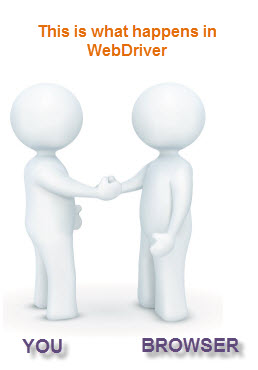
\includegraphics[width=10cm]{Chapter2/Pictures/picture214.jpg}
		\end{center}
		\caption{Kiến trúc của Selenium WebDriver [6]}
		\label{refpicture214}
	\end{figure}
\end{center}


Hình 2.14 mô tả cách làm việc của Selenium WebDriver, lúc này Selenium WebDriver đóng vai trò như người dùng, có nhiệm vụ tương tác tự động với Browser.

\newpage

\subsubsection{Một số ưu nhược điểm của Selenium WebDriver}
\begin{itemize}
	
	\item \textbf{Ưu điểm:}
	
	\begin{itemize}
		\item Giao tiếp trực tiếp với trình duyệt nên tốc độ sẽ rất nhanh.
		\item Tương tác với trình duyệt giống như thao tác của một người dùng thật.
		\item Tốc độ nhanh hơn so với các công cụ Selenium khác.
		\item Thao tác dễ dàng hơn với các phép tính toán logic hay các điều kiện phức tạp.
	\end{itemize}
	
	\item \textbf{Nhược điểm:}
	
	\begin{itemize}
		\item Cài đặt khá phức tạp.
		\item Đòi hỏi người dùng phải có kĩ năng lập trình.\\
	\end{itemize}
\end{itemize}

\subsubsection{Các trình duyệt hỗ trợ Selenium WebDriver}

\begin{center}
	\begin{figure}[htp]
		\begin{center}
			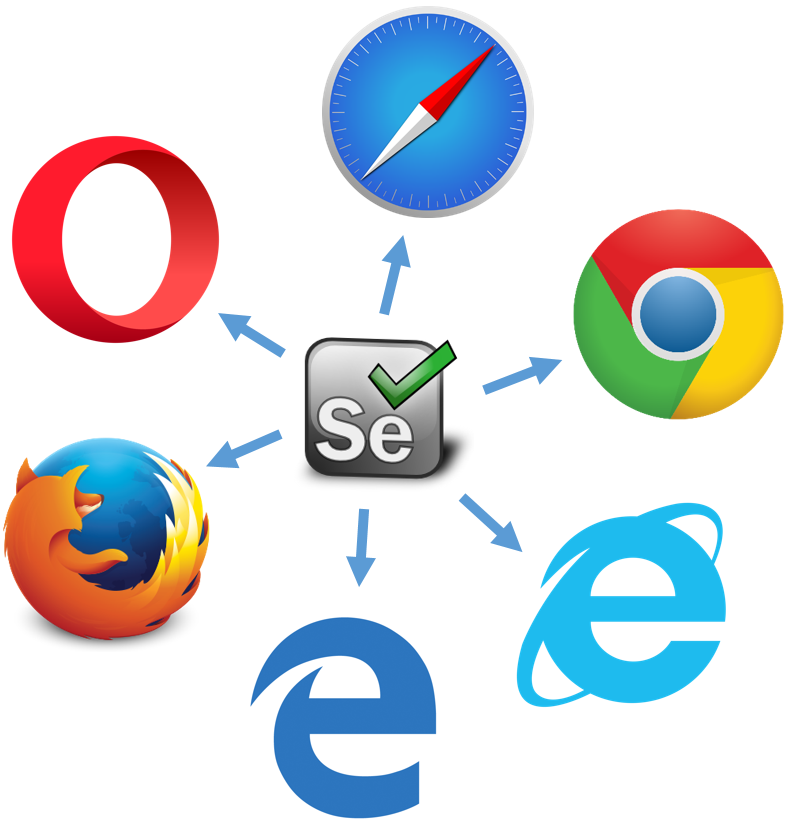
\includegraphics[width=13cm]{Chapter2/Pictures/picture215.png}
		\end{center}
		\caption{Các trình duyệt Selenium WebDriver hỗ trợ hiện nay}
		\label{refpictute215}
	\end{figure}
\end{center}

Selenium WebDriver được hỗ trợ trên rất nhiều các trình duyệt khác nhau. Do đó để sử dụng Selenium WebDriver thì chỉ cần một tập lệnh Selenium và một trình duyệt là đủ. Hình 2.15 thể hiện các trình duyệt hiện nay mà Selenium WebDriver hỗ trợ.

















\chapter{CHỨC NĂNG ĐIỀU KHIỂN CÓ ĐIỀU KIỆN}
\begin{flushleft}
	\fontsize{12pt}{7pt}\selectfont
	\textit{Chương này sẽ trình bày nội dung tích hợp chức năng điều khiển có điều kiện vào công cụ eXe Learning. Mục đầu tiên sẽ nêu các khái niệm điều khiển có điều kiện cùng những hạn chế của eXe và hướng khắc phục. Để tiện cho người đọc có thể hiểu phần hiện thực ở mục thứ ba, mục kế tiếp sẽ trình bày cơ chế hiện thực điều khiển có điều kiện trên SCORM. Cuối cùng là phần hiện thực tính năng ở mục thứ ba.}
\end{flushleft}

\section{Khái niệm về điều khiển có điều kiện trong SCORM}
\subsection{Khái niệm điều khiển có điều kiện (Conditionaly Navigation)}
		

	\begin{center}
	\begin{figure}[htp]
		\begin{center}
			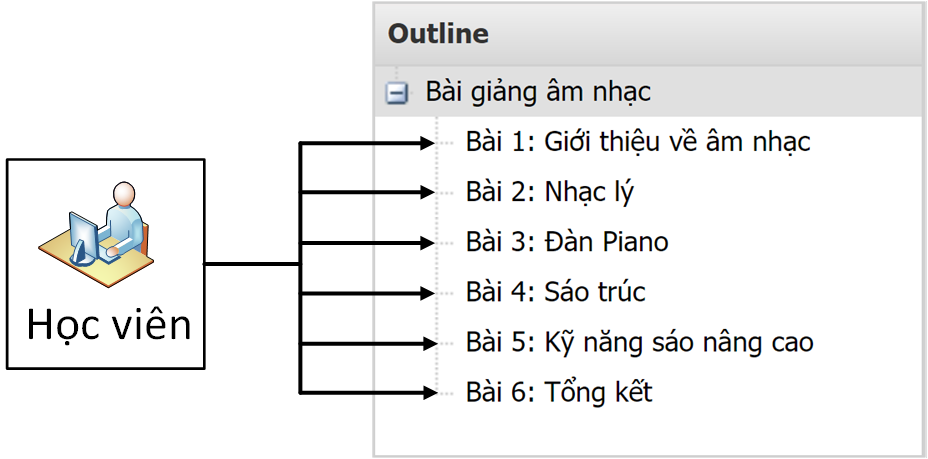
\includegraphics[width=13cm]{Chapter3/Pictures/picture31.png}
		\end{center}
		\caption{Mô hình điều khiển không có điều kiện}
		\label{refpicture12}
	\end{figure}
\end{center}



Hình 3.1 thể hiện ví dụ của một khóa học được soạn thảo bằng eXe hiện tại, khi bắt đầu học, người học có thể ngay lập tức di chuyển vào bất cứ mọi bài trong khóa học. Theo như ví dụ trên thì người học có thể ngay lập tức học \textbf{Bài 6: Tổng kết}, việc này sẽ ảnh hưởng đến thời gian và hiệu suất học tập của người học, vì nếu như chưa trang bị đủ kiến thức của những bài trước mà lại lựa chọn ngay vào học bài tổng hợp ở cuối cùng thì sẽ không đảm bảo việc tiếp thu đầy đủ kiến thức của khóa học. Đây là ví dụ của một mô hình điều khiển không có điều kiện.\\


Chức năng điều khiển có điều kiện sẽ khắc phục được những vấn đề như trên. Chức năng này giúp người soạn thảo có thể thiết lập điều kiện ở mỗi bài, giúp đưa ra một lộ trình học cụ thể. Điều kiện bao gồm tiền điều kiện và hậu điều kiện. Tiền điều kiện là điều kiện mà người học cần thỏa mãn để được vào học một bài học, tiền điều kiện của 1 bài học là bài học mà người học cần phải hoàn thành (thỏa mãn hậu điều kiện) trước khi vào nội dung bài học này. Hậu điều kiện là điều kiện xác nhận người học đã hoàn thành bài học này, hậu điều kiện có thể là thời gian tối thiểu người học phải bỏ ra cho một bài học hoặc phải đạt một số bài kiểm tra nào đó do người biên soạn quy định. Sau đây là ví dụ giúp người đọc dễ hình dung hơn.

\vspace{1cm}

\begin{center}
	\begin{figure}[htp]
		\begin{center}
			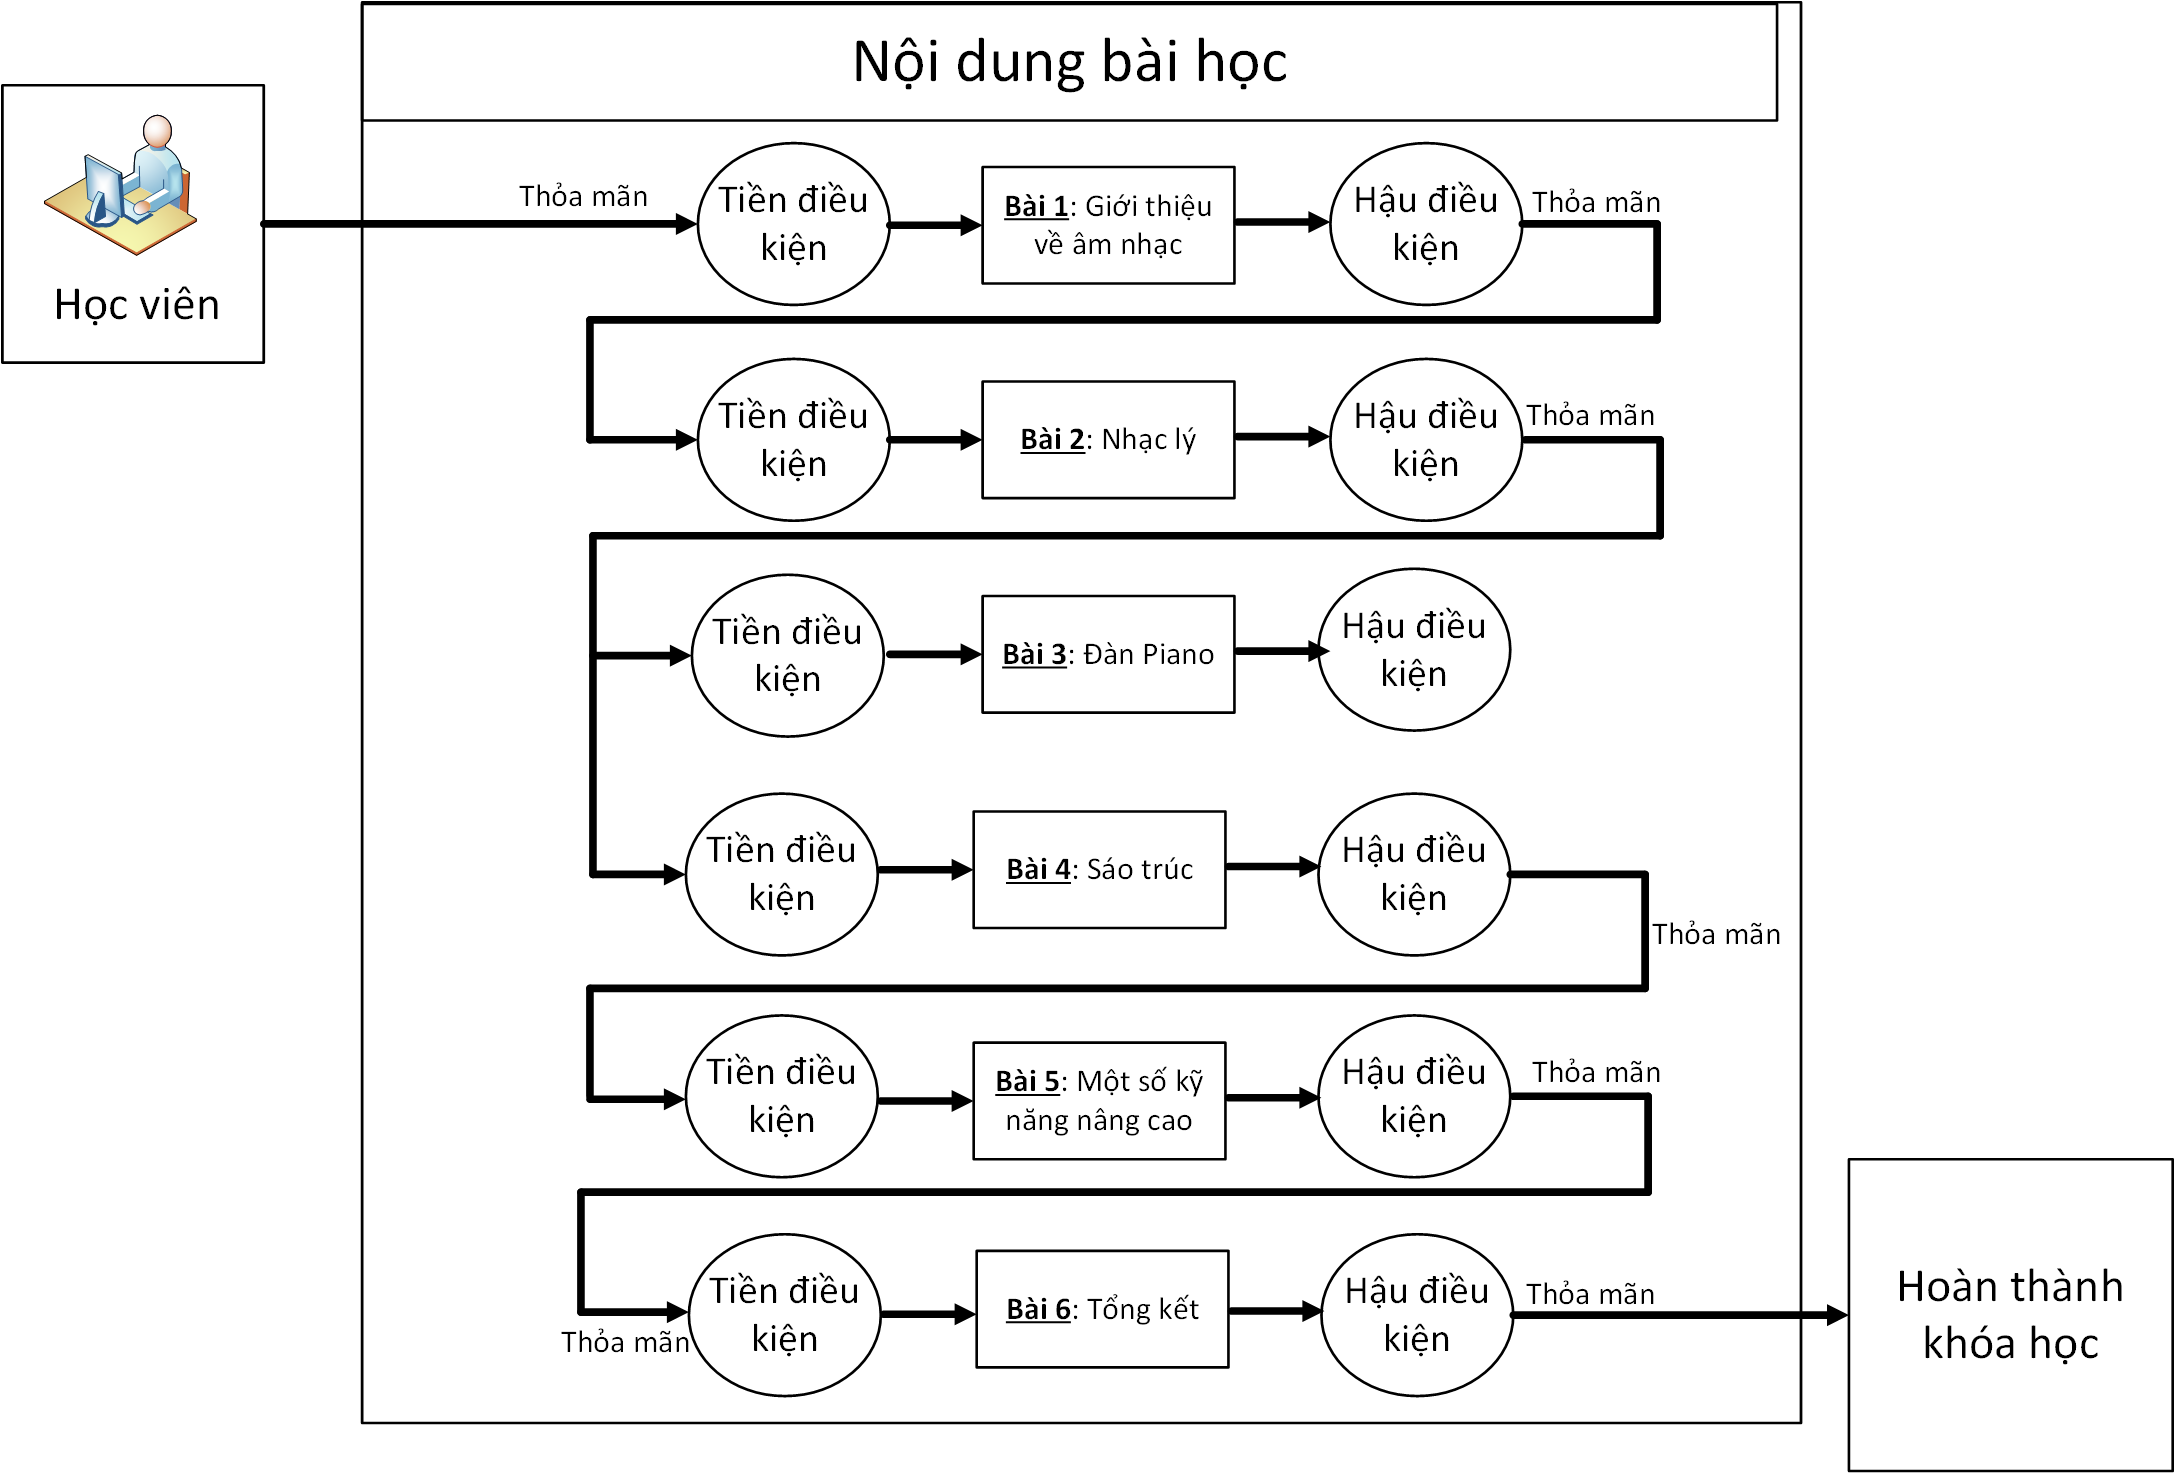
\includegraphics[width=16cm]{Chapter3/Pictures/picture32.png}
		\end{center}
		\caption{Mô hình điều khiển có điều kiện}
		\label{refpicture13}
	\end{figure}
\end{center}


	Hình 3.2 thể hiện ví dụ một mô hình điều khiển có điều kiện. Ở ví dụ này mỗi bài đều được thiết lập tiền điều kiện và hậu điều kiện tương ứng. Đầu tiên học viên sẽ học "Bài 1: Giới thiệu âm nhạc", vì đây là bài đầu tiên của khóa học nên sẽ không cần phải thỏa mãn tiền điều kiện. Tiếp theo học viên muốn học "Bài 2: Nhạc lý" thì học viên cần phải thỏa mãn tiền điều kiện của Bài 2 này, tức hậu điều kiện của Bài 1, hậu điều kiện của Bài 1 có thể là thời gian phải bỏ ra hoặc bài kiểm tra cần đạt tùy theo thiết lập của người soạn thảo. Sau khi hoàn thành Bài 2, học viên có thể lựa chọn tiếp tục học "Bài 3: Đàn Piano" hoặc "Bài 4: Sáo trúc", vì nội dung của 2 bài này độc lập với nhau. Sau khi hoàn thành một trong 2 bài này học viên có thể tiếp tục học "Bài 5: Một số kỹ năng nâng cao" và cuối cùng là "Bài 6: Tổng kết".

\newpage

	Chuẩn SCORM hỗ trợ cho việc xây dựng mô hình điều khiển có điều kiện này bằng cách đưa ra các mô tả dựa vào một tập các thuộc tính, mỗi bài học đều có một tập các thuộc tính này. Mỗi thuộc tính sẽ có hai trạng thái là \textbf{\textit{Enable}} hoặc \textbf{\textit{Disable}} như hình 3.3 mô tả.
	
	\begin{itemize}
		\item \textbf{Enable} là khi các tiền điều kiện của bài này \textbf{\textit{đã được thỏa mãn}} và học viên có thể chọn bài này để học. 
		
		\item \textbf{Disable} là khi các tiền điều kiện của bài học này \textbf{\textit{chưa được thỏa mãn}}, học viên cần phải hoàn thành (thỏa mãn hậu điều kiện) các bài học trước mới có thể vào học bài này. Khi đó bài học này sẽ bị vô hiệu hóa, làm mờ đi và học viên không thể chọn được cho đến khi các tiền điều kiện của nó được thỏa mãn.
	\end{itemize}
	
	

\begin{center}
	\begin{figure}[htp]
		\begin{center}
			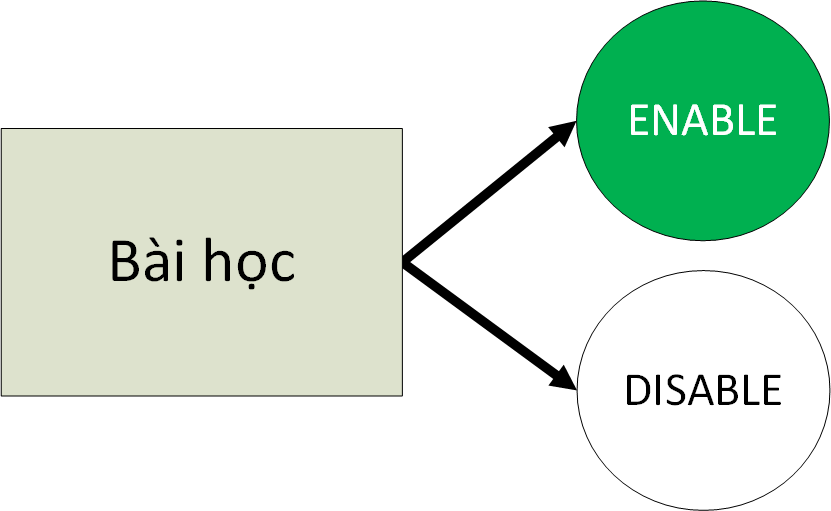
\includegraphics[width=10cm]{Chapter3/Pictures/picture33.png}
		\end{center}
		\caption{Biểu hiện của một bài học đối với người học}
		\label{refpicture42}
	\end{figure}
\end{center}

	
	
\subsection{Mục tiêu đề ra}

	Điều kiện được phát triển để đưa vào mỗi bài học bao gồm hai loại là tiền điều kiện và hậu điều kiện.  Tiền điều kiện là điều kiện mà người học cần thỏa mãn để được vào học một bài học, tiền điều kiện của một bài học là bài học mà người học cần phải hoàn thành (thỏa mãn hậu điều kiện) trước khi vào nội dung bài học này. Hậu điều kiện là điều kiện xác nhận người học đã hoàn thành bài học, hậu điều kiện có thể là thời gian tối thiểu người học phải bỏ ra cho một bài học hoặc phải đạt một số bài kiểm tra nào đó do người biên soạn quy định.\\

	Trong phạm vi Luận Văn này, mục tiêu mà nhóm đặt ra là phát triển các tiền điều kiện và hậu điều kiện nói trên, đồng thời thiết kế giao diện để người soạn thảo đưa các điều kiện này vào bài học và cuối cùng là sinh mã theo chuẩn SCORM có chứa những điều kiện này.

	
\subsection{Các thách thức đặt ra trong quá trình thực hiện}

	Thách thức đầu tiên là sự lỗi thời của các công nghệ được dùng để phát triển eXe. Những công nghệ này đã bị bỏ rơi do cách sử dụng khó khăn, tài liệu hướng dẫn không rõ ràng và phong cách khai báo không tường minh. Bên phía Server, eXe sử dụng hai khung thức của Python là Twisted và Nevow ra đời lần lượt vào năm 2002 và 2004. Còn ở phía Client, eXe sử dụng ExtJS để thiết kế giao diện, ExtJS là một khung thức của Javascript ra đời vào năm 2007. Đây là những công nghệ rất lỗi thời và cộng đồng phát triển của chúng trên Github hầu như không còn. Nevow đã chính thức ngừng phát triển cách đây khoảng năm năm. Tài liệu hướng dẫn của ExtJS rất ít và do đã lâu không cập nhật nên đã bị lỗi thời. \\
	
	Thách thức thứ hai là tài liệu hướng dẫn về những công nghệ này rất hạn chế. Khi tìm kiếm trên google thì số kết quả trả về rất ít, hầu như không có những tài liệu hữu ích và cũng không có những dự án sử dụng những công nghệ này để phát triển. Khi tìm kiếm trên youtube thì hầu như không có Tutorial để tham khảo. Các khóa học về những công nghệ này trên các trang học tập trực tuyến như Udemy, Coursera hay Pluralsight rất ít và cũng không được người học đánh giá cao.\\

	Thách thức thứ ba là cộng đồng phát triển của eXe tương tác rất chậm. Mặc dù diễn đàn của eXe vẫn còn hoạt động nhưng thời gian phản hồi của nó rất chậm do các thành viên phát triển còn rất ít, chỉ có hai người trên diễn đàn này phản hồi với nhóm trong thời gian làm luận văn. Tuy nhiên thời gian nhận được phản hồi cũng rất lâu, khoảng từ hai đến ba tuần cho một vấn đề trong khi thời gian để phát triển luận văn không nhiều.\\
	
	Thách thức thứ tư là hạn chế về thiết kế ban đầu của eXe. Với thiết kế ban đầu của eXe, mỗi bài học chỉ có thể chứa được một SCORM Quiz, hạn chế này đã được các lập trình viên phát triển eXe đưa ra trên diễn đàn theo liên kết \textit{\href{https://exelearning.org/wiki/FAQ}{https://exelearning.org/wiki/FAQ}}. Với thiết kế như vậy, việc người soạn thảo muốn biên soạn nhiều SCORM Quiz trong một bài là không thể. Vì vậy nhóm phải tìm hiểu cách thiết kế ban đầu của iDevice SCORM Quiz trong eXe, sau đó phải tìm cách thay đổi thiết kế này sao cho mỗi bài có thể chứa nhiều SCORM Quiz khác nhau.\\
		


\section{Cơ chế hiện thực chức năng điều khiển có điều kiện}

	SCORM Builder là công cụ hỗ trợ xây dựng dữ liệu theo chuẩn SCORM. SCORM Builder là một công cụ biên soạn (Authoring Tool) cung cấp giao diện soạn thảo bài học, giúp người biên soạn có thể tạo bài giảng, xây dựng nội dung cho bài học và cuối cùng là đóng gói bài học theo chuẩn SCORM. SCORM Builder được sử dụng trong Luận Văn này là eXe.\\
	
	SCORM Engine là công cụ hiển thị nội dung được đóng gói theo chuẩn SCORM. SCORM Engine có thể hiển thị những nội dung mà người soạn thảo đã xây dựng cho bài học, đồng thời tạo ra môi trường giúp nhiều người học có thể tham gia vào bài học này. SCORM Engine được sử dụng trong Luận Văn này là SCORM Cloud.

	
	\begin{center}
	\begin{figure}[htp]
		\begin{center}
			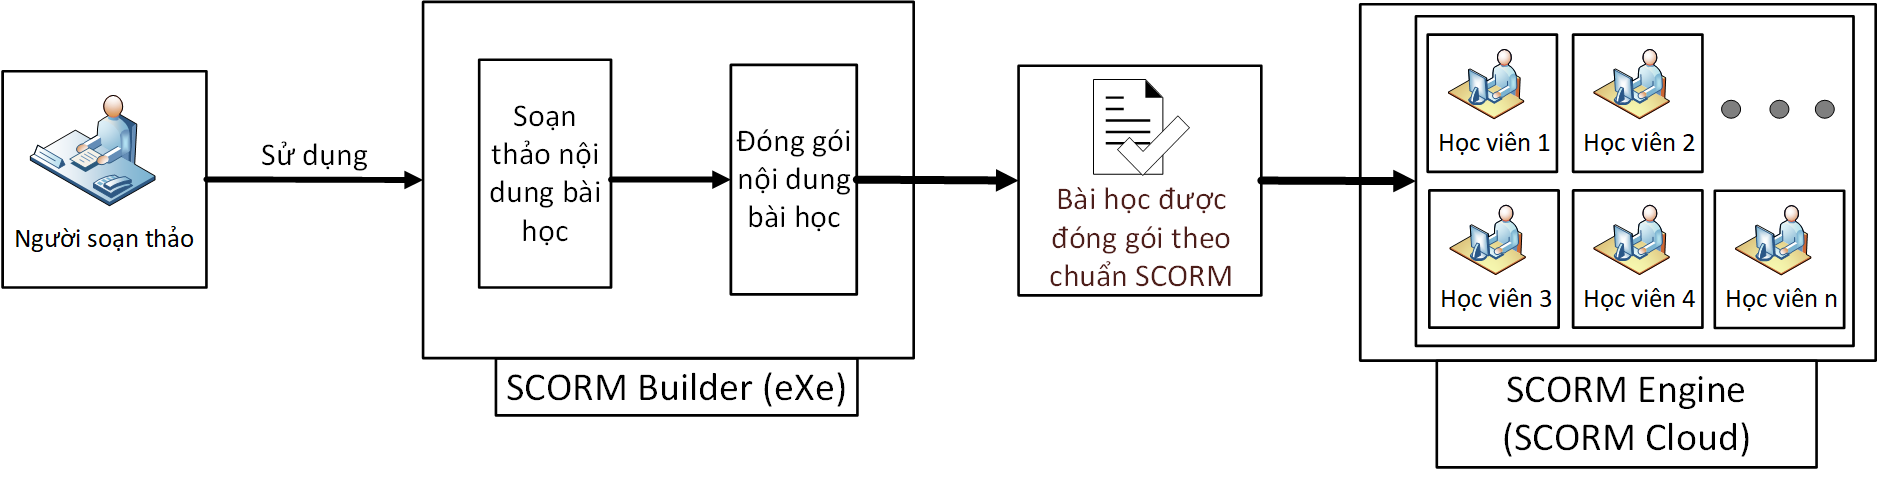
\includegraphics[width=15cm]{Chapter3/Pictures/picture34.png}
		\end{center}
		\caption{Tương tác giữa SCORM Builder và SCORM Engine}
		\label{refpicture45}
	\end{figure}
\end{center}

Hình 3.4 mô tả sự tương tác giữa SCORM Builder và SCORM Engine. Người soạn thảo sẽ sử dụng eXe(SCORM Builder) để thiết kế nội dung cho bài giảng, thêm các tiền điều kiện và hậu điều kiện vào mỗi bài học, sau đó đóng gói bài học theo chuẩn SCORM. Tiếp theo SCORM Cloud(SCORM Engine) sẽ hiển thị nội dung của bài học này và cung cấp một môi trường cho nhiều học viên tương tác với bài học.

\newpage

\subsection{Cấu trúc bài học được đóng gói theo chuẩn SCORM}

	\begin{center}
	\begin{figure}[htp]
		\begin{center}
			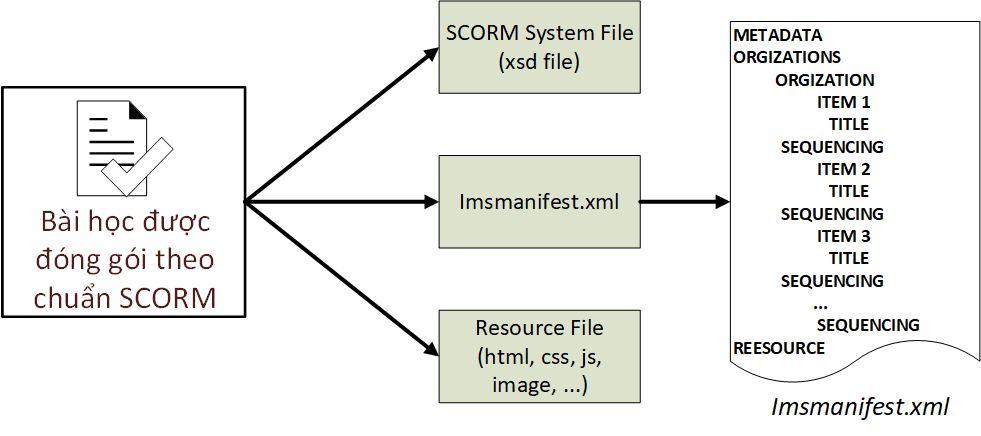
\includegraphics[width=15cm]{Chapter3/Pictures/picture35.png}
		\end{center}
		\caption{Cấu trúc bài học được đóng gói theo chuẩn SCORM}
		\label{refpicture46}
	\end{figure}
\end{center}




	Hình 3.5 liệt kê ở mức tổng quan các thành phần cần phải có trong một gói nội dung theo chuẩn SCORM. Mỗi gói nội dung sẽ bao gồm 3 thành phần chính:
	\begin{itemize}
		\item Thứ nhất là SCORM System File bao gồm những file ở định dạng xsd (XML Schema Defination) chứa những định nghĩa về các thành phần và thuộc tính trong file xml. 
		
		\item Thứ hai là file imsmanifest.xml. Định dạng XML là định dạng mô tả cấu trúc dùng để lưu trữ dữ liệu, đây là file quan trọng nhất trong gói nội dung dùng để chứa các thi6565ết lập về tổ chức nội dung bài học do người soạn thảo biên soạn. 
		
		\item Thành phần cuối cùng là các File tài nguyên sử dụng trong bài học. Các file này là các nội dung chi tiết do người soạn thảo biên soạn, thông thường sẽ là tài nguyên dạng html.
	\end{itemize}
	
	Hình 3.5 cũng cho biết vị trí thiết lập thông tin điều khiển có điều kiện cho mỗi bài học trên cây học tập. Mỗi một bài học trên cây học tập sẽ được ánh xạ tương ứng là một ITEM trong file imsmanifest.xml. Mỗi ITEM sẽ được xác định với một định danh duy nhất dùng để tham chiếu đến tài nguyên tương ứng. Trong mỗi bài học sẽ chứa một đoạn mã điều khiển có điều kiện tương ứng với các thiết lập là các ràng buộc của bài học này.\\
	 
	Sau khi có được gói nội dung được đóng gói theo chuẩn SCORM, theo quy trình như hình 3.4 thì người soạn thảo sẽ upload gói nội dung lên SCORM Cloud để mời học viên tham dự.



\subsection{Cơ chế thể hiện bài học của SCORM Engine}

	Sau khi hoàn thành việc đóng gói các nội dung và các thiết lập. Việc tiếp theo là upload gói nội dung lên SCORM Cloud và mời học viên vào tham gia bài học. Khi có một yêu cầu từ người học thì lúc này SCORM Engine sẽ đứng ra đảm nhận vai trò quản lý quá trình tham gia bài học này.\\

	SCORM Engine là một phần của Hệ Quản trị nội dung đào tạo (LMS). SCORM Engine cung cấp API cho hầu hết các ứng dụng học tập trực tuyến để đọc nội dung theo chuẩn SCORM. SCORM Engine sẽ quản lý các hoạt động như import nội dung, thực hiện khóa học và theo dõi quá trình học tập của người học. Nó là thành phần không thể thiếu đối với bất kỳ hệ thống học tập trực tuyến nào có hỗ trợ chuẩn SCORM.
	
	\begin{center}
	\begin{figure}[htp]
		\begin{center}
			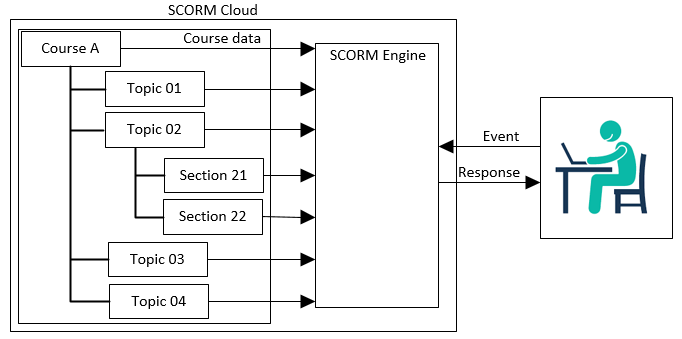
\includegraphics[width=15cm]{Chapter3/Pictures/picture36.png}
		\end{center}
		\caption{Cơ chế hoạt động của SCORM Engine (SCORM Cloud)}
		\label{refpicture47}
	\end{figure}
\end{center}


	
	Khi bắt đầu quá trình học, SCORM Engine sẽ quét tất cả các thành phần của bài học. Các thành phần của bài học này được lưu trữ trên SCORM Cloud từ file imsmanifest.xml đã được upload và các thông tin này được ánh xạ thành mô hình cây bài học như hình 3.6 mô tả.\\
	
	Tiếp đến, SCORM Engine khởi tạo tất cả các thuộc tính ở tất cả các bài học trên cây học tập bao gồm các thuộc tính định danh và thuộc tính trạng thái. SCORM Engine quản lý các thông số bài học theo cơ chế Event-Driven, với mỗi hoạt động của người học thực hiện trên cây học tập thì SCORM Engine sẽ quét lại toàn bộ các thuộc tính trạng thái ở từng bài học của cây học tập và kiểm tra các điều kiện điều khiển đã được thiết lập trên mỗi bài học. Ở từng hoạt động của người học thì các thông tin điều khiển có điều kiện cũng đều được SCORM Engine kiểm tra lại.\\
	
	Mỗi bài học trên cây sẽ có một tập các thuộc tính trạng thái. Những thiết lập điều khiển có điều kiện này sẽ dựa vào tập các thuộc tính này mà đưa ra hai trạng thái là \textbf{\textit{enable}} hoặc \textbf{\textit{disable}} đối với người học. Cụ thể về tập thuộc tính trạng thái này sẽ được trình bày trong phần sau.



\subsection{Cơ chế hiện thực các luật điều khiển có điều kiện}

\subsubsection{Thuộc tính trạng thái trên mỗi bài học}

\begin{center}
	\begin{figure}[htp]
		\begin{center}
			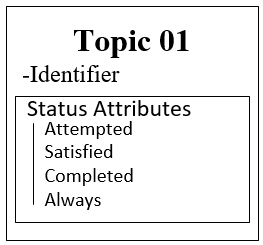
\includegraphics[width=5cm]{Chapter3/Pictures/picture37.png}
		\end{center}
		\caption{Các thuộc tính trong một bài học}
		\label{refpicture48}
	\end{figure}
\end{center}


Mỗi một bài học trên cây học tập ngoài thuộc tính định danh có giá trị duy nhất với mỗi bài học còn có một tập các thuộc tính về trạng thái đối với nhiều trường hợp khác nhau. Hình 3.7 là các thuộc tính có trong một node bao gồm các thuộc tính \textbf{Attempted}, \textbf{Satisfied}, \textbf{Completed} và \textbf{Always}. Các thuộc tính trạng thái này có miền giá trị là Boolean, được dùng để xác định trạng thái của một bài học cụ thể như sau:

\begin{table}[!htp]
	
	\begin{tabular}{|l|p{10.8cm}|}
		\hline 
		\textbf{Thuộc tính trạng thái} & \hspace{4.6cm}\textbf{Ý nghĩa}\\ 
		\hline 
		Attempted & Giá trị khởi tạo là \textbf{False}.\newline \textbf{True} nếu như node bài học này được người học xem qua.
		\\ 
		\hline 
		Satisfied & Giá trị khởi tạo là \textbf{False}.\newline \textbf{True} nếu như node bài học này được người học xem qua và nếu trong node bài học có nội dung cần phải đạt thì điều kiện sẽ \textbf{True} khi đạt các nội dung đó.
		\\ 
		\hline 
		Completed & Giá trị khởi tạo là \textbf{False}.\newline \textbf{True} nếu các nội dung trong node đều được người học xem qua mà không cần phải đạt.
		\\ 
		\hline 
		Always & Giá trị khởi tạo là \textbf{True}.\newline Thuộc tính này không thể thay đổi giá trị. Đây là một thuộc tính được chuẩn SCORM mô tả với mục đính sử dụng riêng.
		\\ 
		\hline 
	\end{tabular} 
	\caption{Các thuộc tính trạng thái của một bài học}
	\label{reftable41}
\end{table}



Nguyên tắc của việc chuyển điều khiển mà chuẩn SCORM mô tả là dựa vào sự thay đổi của các thuộc tính trạng thái này mà đưa ra các hành động tương ứng. Người học và người biên soạn không thể thiết lập giá trị cho các thuộc tính này, các giá trị này sẽ do SCORM Engine quản lý và sẽ thay đổi trong quá trình học của người học. Phần sau sẽ trình bày nguyên tắc SCORM Engine sử dụng các thuộc tính trạng thái này để chuyển trạng thái các node.\\


\subsubsection{Các luật điều khiển có điều kiện}

		\begin{center}
	\begin{figure}[htp]
		\begin{center}
			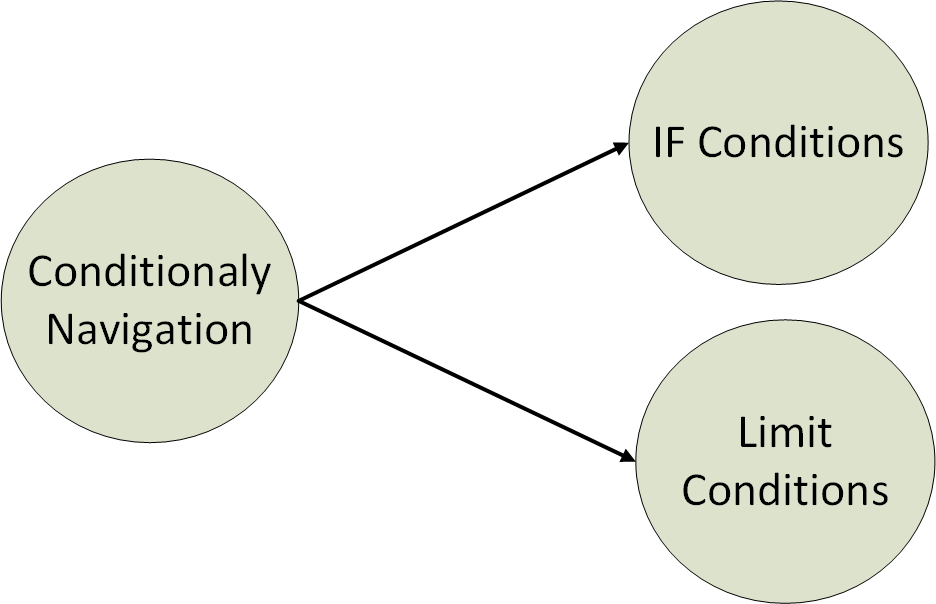
\includegraphics[width=10cm]{Chapter3/Pictures/picture38.png}
		\end{center}
		\caption{Các loại luật điều khiển có điều kiện}
		\label{refpicture49}
	\end{figure}
\end{center}

	Luật điều khiển có điều kiện (Conditionaly Navigation) là một tập hợp gồm không hoặc nhiều điều kiện có thể ảnh hưởng lên bài học trong cây học tập. Có 2 loại luật điều khiển có điều kiện có thể được áp dụng trên các bài học là IF Conditions và Limit Conditions như hình 3.8 mô tả. IF Conditons là tập những ràng buộc dựa vào các trạng thái của các bài học trên cây học tập. Limit Conditions là các ràng buộc về giới hạn, ví dụ như thời gian học trên mỗi bài học và số lần học tập tối đa trên mỗi bài học.\\

 	\textbf{a. IF Conditions}\\
	
	IF Conditions là tập hợp các luật tuân theo cấu trúc \textbf{(IF [condition\_set] THEN [action])}. Hình 3.9 là các tập hợp về những luật điều khiển và các hành động tương ứng được đưa ra. Conditions là các điều kiện được đưa ra dựa trên các thuộc tính trạng thái của các bài học trên cây học tập và các thuộc tính này đã được trình bày ở phần đầu của chương. Rule Actions bao gồm các hành động tương ứng cho các Tiền điều kiện (PreCondition) và Hậu điều kiện (PostCondition). Các thông tin về IF Conditions được đặt trong cặp thẻ <imsss:SequencingRules> trong file imsmanifest.xml theo cấu trúc bài học được đóng gói theo chuẩn SCORM ở hình 3.5.
	
	
		\begin{center}
		\begin{figure}[htp]
			\begin{center}
				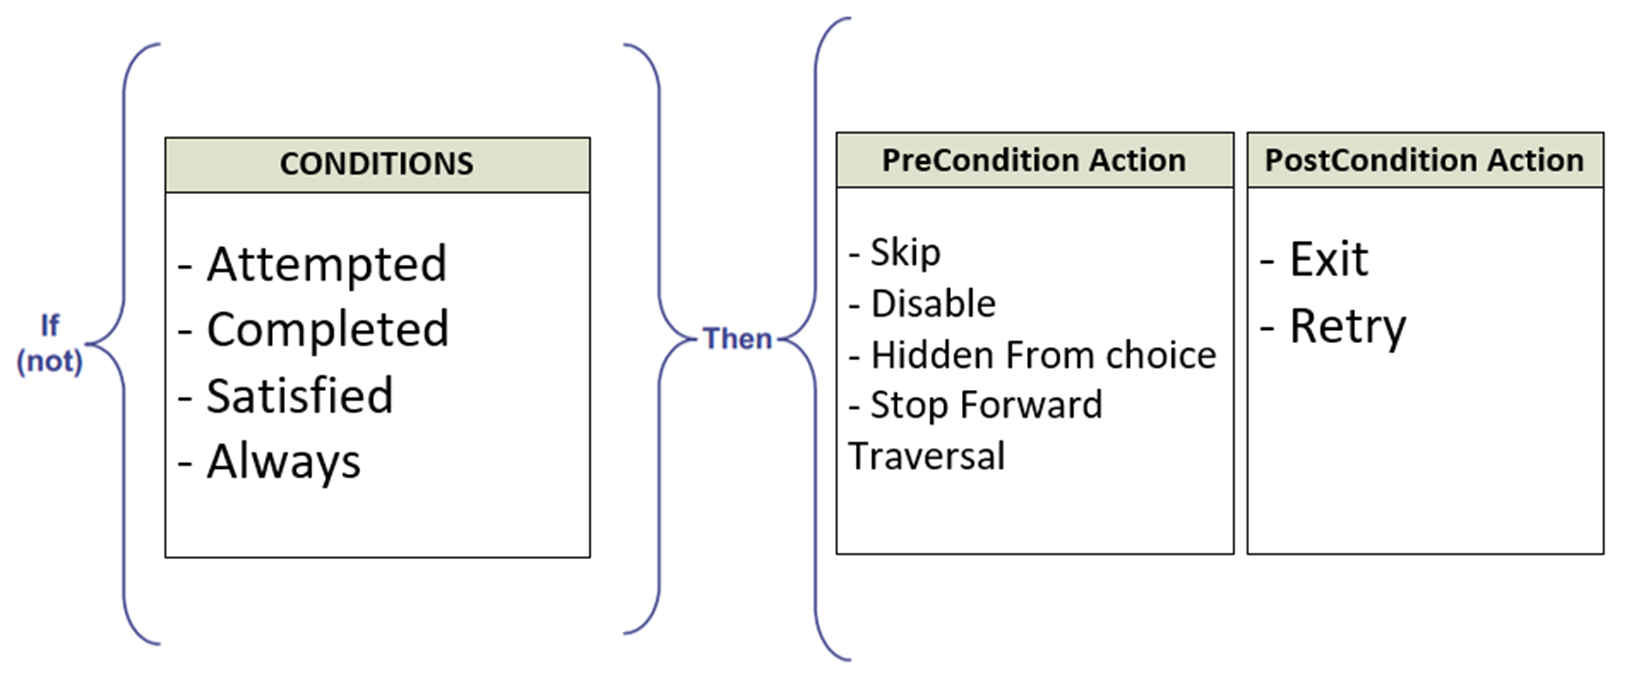
\includegraphics[width=15cm]{Chapter3/Pictures/picture39.png}
			\end{center}
			\caption{Những luật điều khiển và các hành động tương ứng}
			\label{refpicture410}
		\end{figure}
	\end{center}

	Phía sau Then là tập hợp các hành động được SCORM Engine chịu trách nhiệm xử lý khi thỏa mãn điều kiện đưa ra. If Conditions chia các hành động ra thành hai hướng xử lý là hành động cho điều kiện vào và hành động cho điều kiện ra.\\
	
	\begin{itemize}
		\item \textbf{Xử lý cho điều kiện vào}: Tập các hành động đưa ra cho bài học hiện tại để xác định khi nào người học có thể đi vào được bài học này. Ví dụ A có 2 bài học con là B và C, ta thiết lập điều kiện vào trên C là B \textbf{not satisfied} và hành động đưa ra là \textbf{\textit{disable}}. Khi đó, C sẽ bị SCORM Engine \textbf{\textit{disable}} đi cho đến khi các hoạt động trong B \textbf{satisfied} thì C sẽ \textbf{\textit{enable}} và người học có thể lựa chọn.
		
		\item \textbf{Xử lý cho điều kiện ra}: Tập các hành động đưa ra khi đi ra khỏi bài học hiện tại. Ví dụ A có 2 bài học con là B và C, ta thiết lập điều kiện ra ở B là B \textbf{not completed} và hành động đưa ra là \textbf{retry}. Khi đó nếu người học vào B và các hành động trong B chưa được người học xem qua hết thì khi ra khỏi B SCORM Engine sẽ thực hiện lệnh \textbf{retry} và người học sẽ xem lại nội dung B cho đến khi hoàn tất.
	\end{itemize}

	\vspace{1cm}
	
	Có thể kết hợp nhiều Conditons với nhau bằng các toán tử AND hoặc OR. Các toán tử này được thiết lập bằng cách khai báo thêm một thuộc tính \textbf{conditionCombination} khi khai báo cặp thẻ \textbf{<imsss:SequencingRules>. conditionCombination=“any”} cho toán tử OR hoặc \textbf{conditionCombination=“all”} cho toán tử AND.\\
	
	Với mỗi trường hợp ta sẽ có tập hợp những hành động đưa ra tương ứng. Các hành động này được liệt kê như trong bảng 3.2.
	
	\newpage
	
\begin{table}[!htp]
	
	\begin{tabular}{|p{4cm}|p{10.8cm}|}
		\hline 
		\textbf{Trường hợp} & \hspace{4.6cm}\textbf{Hành động} 
		\\
		\hline 
		Xử lý điều kiện vào của bài học hiện tại. & 
		\textbf{\textit{Skip}} – bài học hoạt động này sẽ không được tham gia vào trình duyệt cây.\newline
		\textbf{\textit{Disabled}} – Hoạt động này sẽ bị vô hiệu hóa và không thể tham gia vào quá trình duyệt cây.\newline
		\textbf{\textit{Hidden from Choice}} – Hoạt động này sẽ không thể bị target và bị ẩn khỏi cây.\newline
		\textbf{\textit{Stop Forward Traversal}} – Không cho phép duyệt các phần tử con của bài học Activity này.
		\\
		\hline 
		Xử lý điều kiện ra khi thoát khỏi bài học hiện tại. & 
		\textbf{\textit{Exit}} – Action thoát khỏi nội dung này bình thường.\newline
		\textbf{\textit{Retry}} – Action đưa yêu cầu làm lại nội dung này.
		\\
		\hline 
	\end{tabular} 
	\caption{Các điều kiện và hành động tương ứng của một bài học}
	\label{reftable42}
\end{table}	
	

 \textbf{b. Limit Conditions}\\
	
	Limit Conditions đưa ra các ràng buộc về giới hạn cho bài học hiện tại trên cây học tập. Limit Conditions chỉ ra các thông số giới hạn mà người học có thể thực hiện được như số lần làm bài tối đa, thời gian học tối thiểu trong một nội dung. Được đặt trong cặp thẻ <LimitConditions> trong file imsmanifest.xml.\\
	
	Chuẩn SCORM quy định có 2 ràng buộc về điều kiện giới hạn như sau:
	
	\begin{itemize}
		\item \textbf{Attempt Limits}: Ràng buộc về số lần học tối đa đối với một nội dung. Được hiện thực bằng 2 tham số: 
			\begin{itemize}
				\item \textbf{Limit Condition Attempt Control:} có giá trị Boolean để quy định rằng nội dung này có bị ảnh hưởng bởi ràng buộc Limit Condition này hay không. 
				
				\item \textbf{Limit Condition Attempt Limit:} có giá trị là Non-negative Interger quy định số lần học tối đa đối với một nội dung. Ví dụ nếu tham số này có giá trị 3 thì người học có thể xem nội dung này 3 lần trong quá trình học.
				
			\end{itemize}
			
		\item \textbf{Attempt Absolute Durations:} Ràng buộc về thời gian học tối thiểu đối với một nội dung trong cây học tập. Được hiện thực bằng 2 tham số: 
			\begin{itemize}
	
				\item \textbf{Limit Condition Attempt Absolute Duration Control:} có giá trị Boolean để quy định rằng nội dung này có bị ảnh hưởng bởi ràng buộc Limit Condition này hay không. 
				
				\item \textbf{Limit Condition Attempt Absolute Duration Limit:} có giá trị là Duration với Acurarcy 0.1 second quy định thời gian tối thiểu đối với một nội dung. Nếu thiết lập giá trị là 60s thì người học phải xem nội dung này tối thiểu trong một phút mới có thể chuyển sang nội dung tiếp theo.

			\end{itemize}
		
	\end{itemize}
	
	\newpage
	

\section{Hiện thực chức năng}


		\begin{center}
	\begin{figure}[htp]
		\begin{center}
			
\includegraphics[width=15cm]{Chapter3/Pictures/picture310.png}
		\end{center}
		\caption{Quy trình hiện thực chức năng điều khiển có điều kiện}
		\label{refpicture413}
	\end{figure}
\end{center}


	Hình 3.10 là quy trình hiện thực chức năng do nhóm đề xuất thực hiện. Bao gồm bốn bước chính. Bước một là xác định các tiền điều kiện và hậu điều kiện cần thiết để đưa vào bài học. Ở bước hai sẽ thiết kế giao diện dành cho người soạn thảo có thể đưa các điều kiện này vào trong bài học. Bước ba là xử lý việc lưu trữ thông tin của bài học đã được thêm các điều kiện vào. Bước cuối cùng sẽ dựa vào những điều kiện đã lưu để sinh mã có chức năng điều khiển có điều kiện cho từng bài.\\
	
	
	
\subsection{Xác định các tiền điều kiện và hậu điều kiện}

	Sau khi tìm hiểu các ràng buộc về điều khiển có điều kiện có trong đặc tả chuẩn SCORM 2004. Nhóm đưa ra các ràng được sẽ được hiện thực trong chức năng. Tiền điều kiện là các ràng buộc cần để có thể vào được nội dung này. Hậu điều kiện là các ràng buộc để ra khỏi nội dung này.


\begin{itemize}
	\item \textbf{PreCondition (Tiền điều kiện):} Ràng buộc về nội dung trước cần thõa mãn. Ví dụ A có 2 bài học con là B và C, ta set PreCondition trên C là B \textbf{\textit{satisfied}}. Khi đó  các hoạt động trong B nếu \textbf{NOT} \textbf{\textit{satisfied}} thì action là C \textbf{\textit{disable}}.
	
	\item \textbf{PostConditon (Hậu điều kiện):}
	\begin{itemize}
		\item Ràng buộc về thời gian học trong một bài học. Nếu trong bài học có thiết lập thời gian học, người học sẽ không thể ra khỏi nội dung này nếu chưa hết thời gian quy định.
		
		\item Nếu trong bài học có SCORM Quiz thì đưa ra những lựa chọn ràng buộc về SCORM Quiz, bao gồm các tùy chỉnh: Đạt một hoặc nhiều SCORM Quiz, các SCORM Quiz cần đạt này do người biên soạn quy định hoặc đạt một trong số các SCORM Quiz có trong bài học.
	\end{itemize}

	
\end{itemize}

	Sau khi xác định được các ràng buộc sẽ thể hiện trong chức năng, phần tiếp theo sẽ trình bày quá trình hiện thực chức năng bao gồm 3 bước còn lại trong quy trình đưa ra ở hình 3.10.


\subsection{Thiết kế giao diện để đưa các điều kiện vào trong bài học}

	Giao diện Sequencing Config sẽ là duy nhất  đối với từng bài học. Với những bài học có SCORM Quiz sẽ có thêm các thiết lập về SCORM Quiz, những bài học không có SCORM Quiz sẽ không xuất hiện những tùy chọn này.\\
	
	Giao diện Sequencing Config sẽ có hai Tag Panel chính là PreCondition và PostCondition. PreCondition chứa thiết lập về tiền điều kiện và PostCondition chứa thiết lập về hậu điều kiện cho bài học.\\
	
	Hình 3.11 là giao diện thiết lập tiền điều kiện, giao diện này sẽ có một combo box yêu cầu chọn nội dung trước cần thỏa mãn, người học cần thỏa mãn nội dung được chọn mới được vào học bài này.

		\begin{center}
	\begin{figure}[htp]
		\begin{center}
			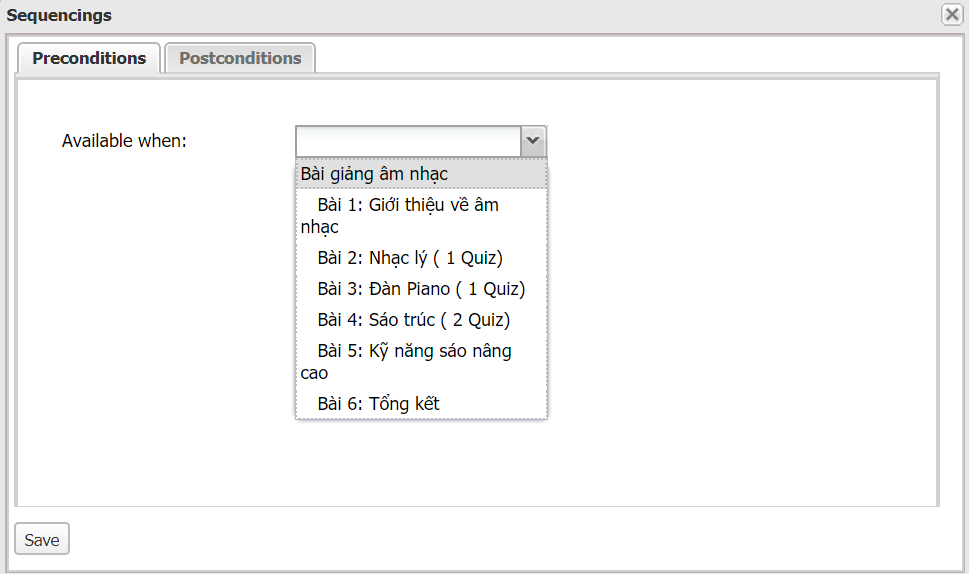
\includegraphics[width=15cm]{Chapter3/Pictures/picture311.png}
		\end{center}
		\caption{Giao diện thiết lập tiền điều kiện}
		\label{refpicture413}
	\end{figure}
\end{center}

	Khi giao diện thiết lập tiền điều kiện này xuất hiện, trình duyệt sẽ gửi yêu cầu rằng người soạn thảo đang cần thực hiện các thiết lập điều khiển có điều kiện, lúc này máy chủ thông qua việc sử dụng kỹ thuật Ajax để lấy dữ liệu. Máy chủ sẽ phân tích yêu cầu này và gửi danh sách các bài học có trong khóa học lưu dưới dạng JSON cho trình duyệt. Trình duyệt sẽ phân tích nội dung nhận được này và thể hiện thành các mục trong combobox.


		\begin{center}
	\begin{figure}[htp]
		\begin{center}
			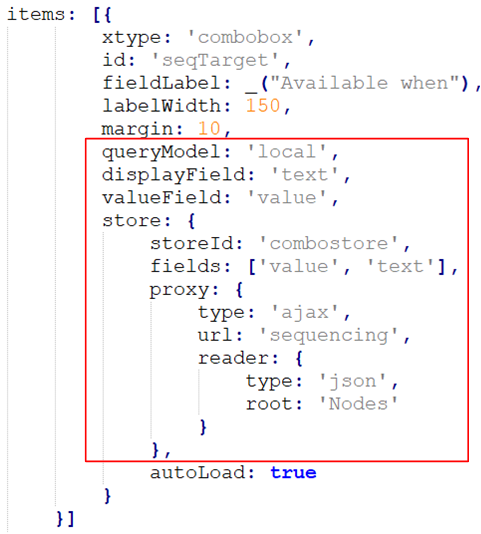
\includegraphics[width=7cm]{Chapter3/Pictures/picture312.png}
		\end{center}
		\caption{Kỹ thuật Ajax để lấy dữ liệu trong combobox}
		\label{refpicture413}
	\end{figure}
\end{center}


	Hình 3.12 là đoạn mã hiện thực combobox trong giao diện thiết lập tiền điều kiện sử dụng khung thức của ExtJS để hiện thực. Ở đây, dữ liệu JSON lấy từ url:sequencing sẽ được lưu trữ thành một data store có ID là "combostore" gồm 2 trường “value” và “text”. Combobox sẽ lấy trường hiển thị (display Fiels) là trường “text” và trường giá trị(valueField) là “value”. Hình 3.13 là cú pháp combobox đối chiếu với Javascript thuần túy.

		\begin{center}
	\begin{figure}[htp]
		\begin{center}
			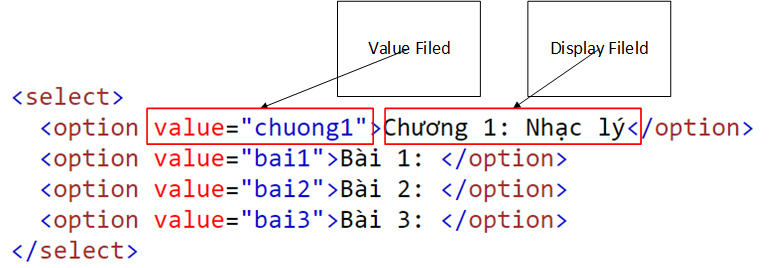
\includegraphics[width=15cm]{Chapter3/Pictures/picture313.png}
		\end{center}
		\caption{Combobox theo Javascript thuần túy}
		\label{refpicture413}
	\end{figure}
\end{center}


		\begin{center}
	\begin{figure}[htp]
		\begin{center}
			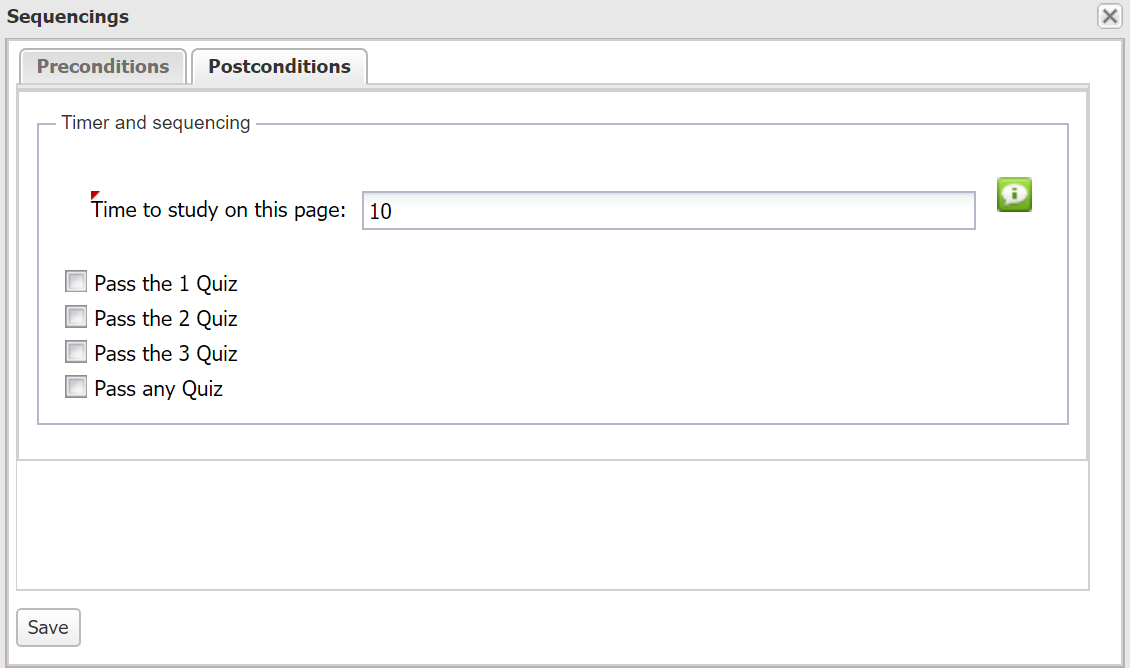
\includegraphics[width=15cm]{Chapter3/Pictures/picture314.png}
		\end{center}
		\caption{Giao diện thiết lập hậu điều kiện}
		\label{refpicture415}
	\end{figure}
\end{center}


Hình 3.14 là giao diện thiết lập các hậu điều kiện. Giao diện này sẽ có một textField yêu cầu người soạn thảo nhập vào thời gian tối thiểu mà người học sẽ phải xem nội dung này, đơn vị của thời gian sẽ tính bằng giây.
Nếu như trong nội dung bài học này mà người soạn thảo có thiết lập SCORM Quiz thì các thiết lập về SCORM Quiz sẽ xuất hiện ở đây bao gồm các checkbox yêu cầu cần đạt đối với từng SCORM Quiz và có thêm checkbox “Pass any Quiz” cho điều kiện chỉ cần đạt một trong bất kỳ SCORM Quiz nào là nội dung này sẽ được thõa mãn. Sau khi lấy các thông số người dùng nhập vào, sử dụng các phương thức gửi và nhận dữ liệu do Nevow cung cấp để gửi và lưu trữ thông tin ở phía máy chủ.


\subsection{Lưu thông tin bài học do người soạn thảo thiết lập}

Như đã trình bày ở phần kiến trúc hệ thống công cụ eXe Learning. Hệ thống hoạt động theo mô hình Client-Server và các phương thức xử lý đều được thực hiện ở phía Server. Sau khi người soạn thảo thiết lập các điều kiện điều khiển trình tự ở bước trên, thì dữ liệu này sẽ phải được gửi về phía server để tiến hành bước tiếp theo.

		\begin{center}
	\begin{figure}[htp]
		\begin{center}
			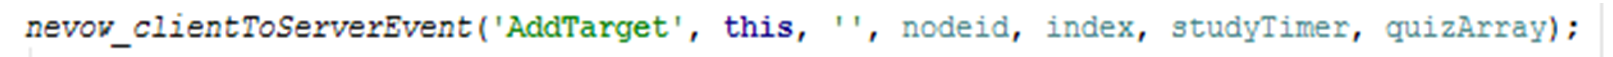
\includegraphics[width=15cm]{Chapter3/Pictures/picture315.png}
		\end{center}
		\caption{Phương thức Nevow gửi dữ liệu về Server}
		\label{refpicture416}
	\end{figure}
\end{center}

	Hình 3.15 là phương thức gửi dữ liệu về phía máy chủ được Nevow cung cấp, Các thuộc tính lần lượt là nodeid, index, studyTimer, quizList với nodeid là IdTarget lưu trữ bài học mục tiêu cần thỏa mãn của bài học hiện tại, index là vị trí của bài học hiện tại trên cây bài học, studyTimer lưu trữ thời gian học tối đa trong bài học hiện tại và quizList lưu trữ danh sách các Quiz cần Pass của bài học hiện tại nếu có.\\

	
	Như vậy, cần thay đổi các thiết kế ban đầu về một số cấu trúc lưu trữ dữ liệu ở phía server để có thể lưu trữ được các nội dung này. Như đã trình bày eXe Learning quản lý nội dung của các bài học theo mô hình cây. Mỗi bài học trong khóa học sẽ được lưu trữ là một bài học trong cây học tập. Mỗi bài học sẽ được thêm ba thuộc tính tương ứng với ba điều kiện điều khiển có điều kiện.


		\begin{center}
	\begin{figure}[htp]
		\begin{center}
			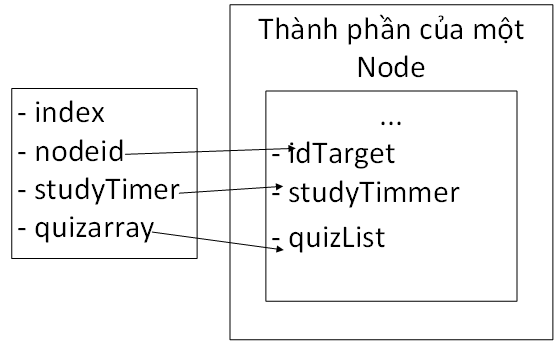
\includegraphics[width=15cm]{Chapter3/Pictures/picture316.png}
		\end{center}
		\caption{Lưu trữ các thiết lập trên bài học}
		\label{refpicture413}
	\end{figure}
\end{center}

Hàm xử lý nhận các tham số mà hình 3.15 cung cấp sẽ được hiện thực như hình 3.16 mô tả. Đầu tiên sẽ dựa vào tham số index nhận được, tìm ra bài học cần thiết lập. Sau khi tìm vị trí bài học hiện tại được lưu trữ trên máy chủ thông qua tham số index nhận được, máy chủ sẽ lưu trữ các tham số tiếp theo trong bài học vừa tìm được. idTarget là thuộc tính cho bài học mục tiêu cần thõa mãn. studyTimer là thuộc tính cho thời gian học tối thiểu. quizList là danh sách các quiz cần phải đạt để nội dung này thỏa mãn.



\subsection{Sinh mã điều khiển có điều kiện theo chuẩn SCORM}

	Như đã trình bày ở phần đầu chương, các đoạn mã điều khiển có điều kiện được tạo ra trong file imsmanifest.xml. Phương thức sinh ra chuỗi để ghi vào file này được hiện thực trong module Export. \\
	
	File scormexport.py khai báo hai lớp chính là Manifest và ScormExport. Lớp Manifest chứa các phương thức sinh mã ra file imsmanifest.xml. Lớp ScormExport chứa các phương thức gộp các file thành phần lại với nhau và đóng gói thành file có định dạng zip. Mã điều khiển có điều kiện được sinh ra trong file imsmanifest.xml, do đó nhóm sẽ hiện thực thêm một phương thức để sinh ra các đoạn mã này trong class Manifest. Quá trình sinh ra các đoạn mã này như sau:

	
	\begin{center}
	\begin{figure}[htp]
		\begin{center}
			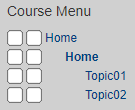
\includegraphics[width=4cm]{Chapter3/Pictures/picture317.png}
		\end{center}
		\caption{Course Menu trong ví dụ}
		\label{refpicture411}
	\end{figure}
\end{center}


Đây là một ví dụ tổng hợp về các luật điều khiển có điều kiện mà chuẩn SCORM mô tả đã trình bày ở các phần trên. Hình 3.17 là mô hình cây học tập được đưa ra trong ví dụ gồm 1 nội dung với 2 topic là \textbf{Topic01} và \textbf{Topic02}.


\begin{center}
	\begin{figure}[htp]
		\begin{center}
			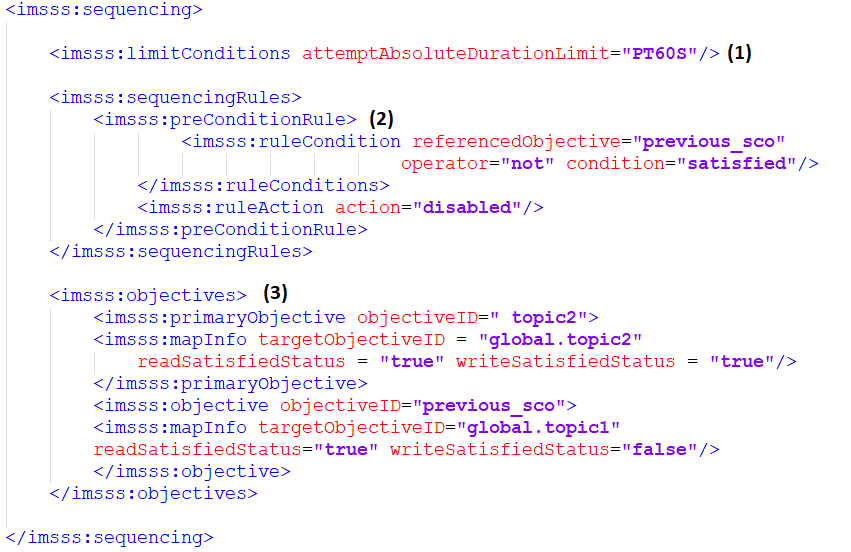
\includegraphics[width=15cm]{Chapter3/Pictures/picture318.png}
		\end{center}
		\caption{Đoạn mã chứa thông tin điều khiển có điều kiện trong file imsmanifest.xml}
		\label{refpicture412}
	\end{figure}
\end{center}

\newpage

Hình 3.18 là những đặc tả về thông tin điều khiển có điều kiện theo chuẩn SCORM được trình bày sang file imsmanifest.xml. XML là ngôn ngữ cấu trúc dùng để chứa dữ liệu và liệt kê các thành phần dữ liệu, do đó cấu trúc IF [conditions\_set] THEN [Action] sẽ không có hình thái rõ ràng như các ngôn ngữ khác. File imsmanifest.xml này sẽ chỉ lưu dữ liệu của cấu trúc trên và việc thực thi sẽ do SCORM Engine thực hiện.\\

Đoạn mã trong hình 3.18 được đặt trong <item> có định danh là \textbf{\textit{topic2}}, tương ứng với \textbf{Topic02} trên cây học tập ở hình 3.17. Đoạn mã trên có 3 phần riêng biệt với các nhiệm vụ khác nhau. \\

Phần \textbf{(3)} là phần khai báo các đối tượng sử dụng bao gồm một primary Object và một Object. Khai báo Primary Object là khai báo định danh cho chính Item hiện tại, ở đây là \textbf{\textit{topic2}}. Khi thực thi, trên bài học này cho phép SCORM Engine có thể đọc và ghi thuộc tính \textbf{\textit{satisfied}}. Khai báo Objective là khai báo các đối tượng tham chiếu đến, ở đây khai báo có tên là \textbf{\textit{previous\_sco}} dùng để tham chiếu đến bài học nội dung có định danh là \textbf{\textit{topic1}}. Khi thực thi trên bài học này chỉ có thể đọc thuộc tính \textbf{\textit{satisfied}} của Object Topic01 nhưng không thể ghi thuộc tính \textbf{\textit{satisfied}} của \textbf{Topic01}.\\

Phần \textbf{(2)} là triển khai các điều kiện vào với điều kiện đưa ra là \textbf{\textit{previous\_sco}} \textbf{NOT} \textbf{satisfied} và hành động đưa ra là \textbf{\textit{disable}}. Khi định danh mà \textbf{\textit{previous\_sco}} tham chiếu đến là \textbf{\textit{topic1}} chưa thỏa mãn thì \textbf{\textit{topic2}} sẽ bị \textbf{disable}. Khi nào các thành phần trong \textbf{\textit{topic1}} đã thỏa mãn yêu cầu thì \textbf{\textit{topic2}} sẽ được đưa vào lựa chọn.\\

Phần \textbf{(1)} là triển khai Limit Conditions với điều kiện đưa ra là Limit Condition Attempt Absolute Duration Limit = 60 second. Điều kiện này quy định thời gian học đối với topic 2 này là 60s.



\subsection{Kết quả thực hiện}

Sau khi đóng gói nội dung khóa học có các thông tin điều khiển có điều kiện bằng công cụ eXe. Nhóm tiến hành upload lên SCORM Cloud để xem kết quả và so sánh với gói nội dung không có thông tin điều khiển có điều kiện.	
	
			\begin{center}
		\begin{figure}[htp]
			\begin{center}
				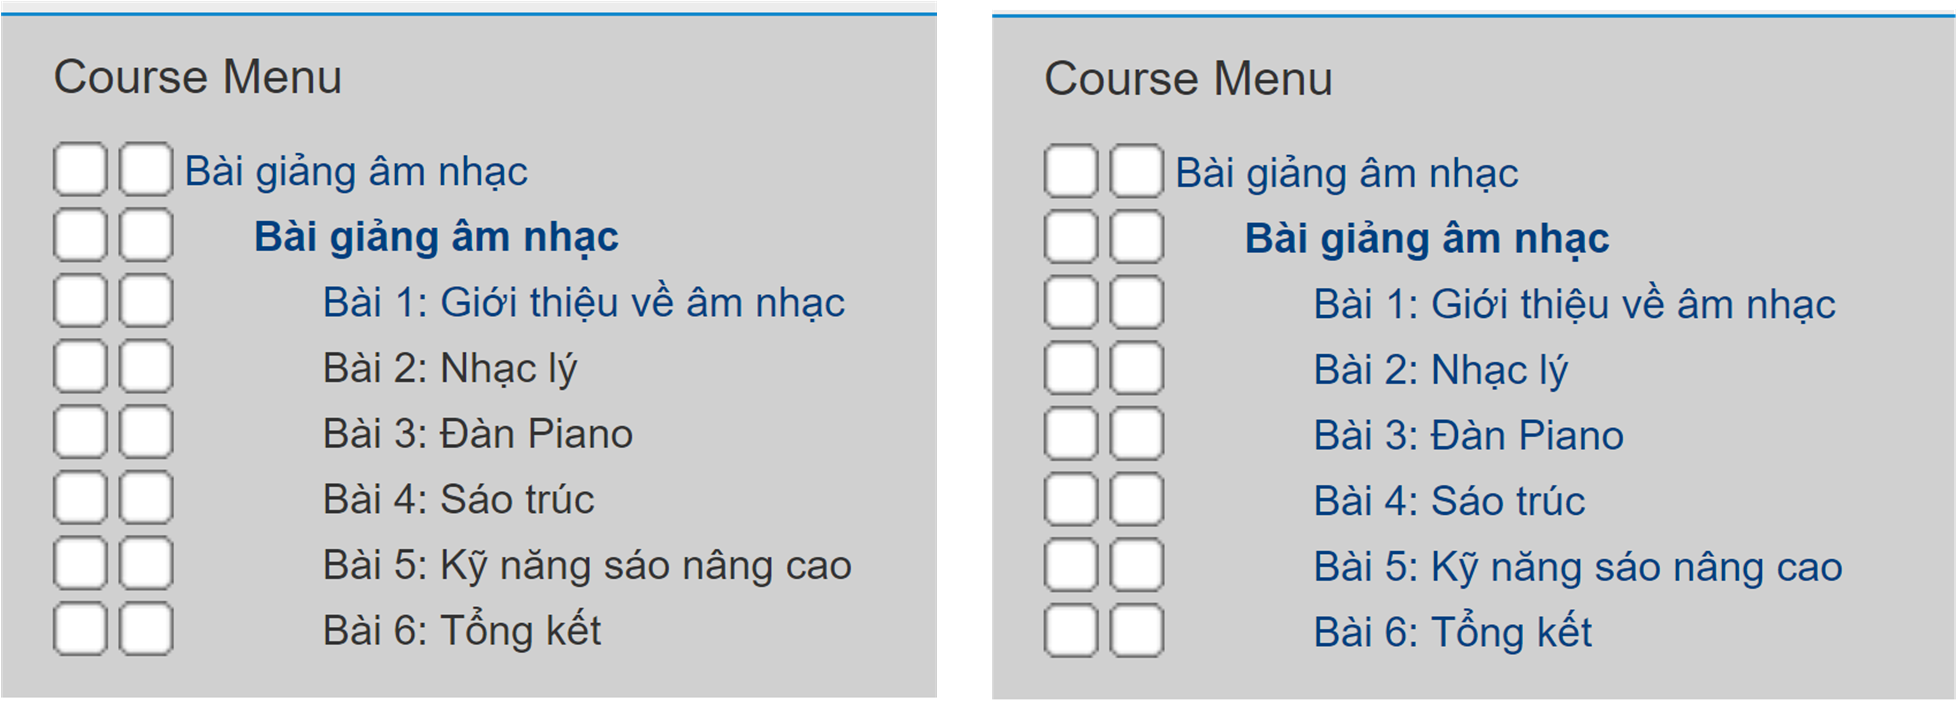
\includegraphics[width=15cm]{Chapter3/Pictures/picture319.png}
			\end{center}
			\caption{Giao diện của hai khóa học trên SCORM Cloud}
			\label{refpicture417}
		\end{figure}
	\end{center}
	
	Hình 3.19a là khóa học không có thông tin điều khiển có điều kiện và hình 3.19b là khóa học đã thiết lập thông tin điều khiển có điều kiện. Rõ ràng ta thấy hình 3.19b yêu cầu người học phải tuân theo một lộ trình do người biên soạn thiết lập sẵn. Trong mỗi bài học sẽ có những yêu cầu riêng như học trong một khoản thời gian nhất định hoặc pass các bài quiz có trong bài học hoạt động. Còn hình 3.19a thì người học có thể tham gia vào bất kì hoạt động nào có trên cây.

\subsection{Hạn chế của chức năng}	

	Chưa đi sâu vào nghiên cứu ý kiến và nhu cầu của người biên soạn. Nhu cầu của người biên soạn đóng vai trò quan trọng trong việc thiết kế chức năng của ứng dụng. Do cộng đồng người sử dụng eXe Learning tương tác với nhau khá chậm nên nhóm gặp rất nhiều khó khăn trong việc tiến hành thu thập thông tin về nhu cầu của người sử dụng. \\
	
	Nhóm chỉ tập trung vào nghiên cứu và thực hiện một số ràng buộc tương đối đơn giản.  Chưa khai thác được hết toàn bộ sức mạnh của các mã SCORM được đặc tả trong chuẩn SCORM, không sử dụng được hết tất cả các Rule Conditions (Luật điều kiện) là một trong những hạn chế lớn của chức năng.









\chapter{CHỨC NĂNG TỔNG HỢP CÂU HỎI VÀ TẠO BÀI KIỂM TRA}
\begin{flushleft}
	\fontsize{12pt}{7pt}\selectfont
	\textit{Chương này sẽ trình bày chức năng tổng hợp câu hỏi và tạo bài kiểm tra. Mục đầu tiên sẽ trình bày về thiết kế của iDevice SCORM Quiz được tích hợp sẵn trong hệ thống eXe Learning cùng những ưu, nhược điểm của SCORM Quiz và hướng khắc phục nhược điểm của nó. Mục tiếp theo sẽ trình bày cách thiết kế iDevice SCORM Test, một iDevice có thể tạo bài kiểm tra có các câu hỏi động từ các SCORM Quiz đã có.}
\end{flushleft}

\section{Đặt vấn đề}
\subsection{Chức năng kiểm tra kiến thức hiện tại của eXe Learning}
	Trong việc thiết kế bài học E-Learning, nhu cầu kiểm tra kiến thức của người học sau mỗi bài học là rất cần thiết. Qua đó có thể biết được người học đã tiếp thu được bao nhiêu kiến thức do người soạn thảo trình bày trong bài học. Do đó, cần có một công cụ cung cấp chức năng soạn thảo câu hỏi cho người biên soạn. eXe cung cấp SCORM Quiz với nhiệm vụ và chức năng nói trên.\\

	SCORM Quiz là một trong số các công cụ kiểm tra được thiết kế sẵn trong eXe Learning. Mục đích hướng đến của SCORM Quiz là giúp người soạn thảo có thể biên soạn các câu hỏi ôn tập một cách đơn giản, cho người học biết được số điểm họ làm được sau thi thực hiện xong. Các câu hỏi được biên soạn theo hình thức Mutiple Choice với một câu hỏi và nhiều hơn một lựa chọn, trong đó chỉ có một lựa chọn đúng.\\

	Bên cạnh các ưu điểm kể trên, so với các công cụ kiểm tra có trong các phần mềm soạn thảo bài giảng E-Learning khác thì SCORM Quiz vẫn còn rất nhiều nhược điểm. Sau đây sẽ trình bày về một số ưu điểm cũng như nhược điểm mà SCORM Quiz tồn tại.


\subsection{Nhược điểm của SCORM Quiz }

	Nhược điểm lớn nhất trong thiết kế SCORM Quiz là người biên soạn chỉ có thể thiết lập một SCORM Quiz cho mỗi bài học. Đây là do quan điểm thiết kể của những người phát triển eXe Learning với mỗi bài học sẽ chỉ có được một SCORM Quiz đi cùng. Nhận thấy đây là một thiết kế không linh hoạt với nhu cầu soạn thảo. Nếu như trong một bài học có hai nội dung cần đặt câu hỏi thì với một SCORM Quiz là không đủ.\\
	
	Thứ hai là SCORM Quiz không có thuộc tính phân loại cho các câu hỏi. Về mặt khách quan người soạn thảo sẽ rất khó khăn trong việc đánh giá mức độ của bài trắc nghiệm. Hơn nữa khi người biên soạn xem lại bài học đã soạn thảo từ trước sẽ rất tốn thời gian phân loại và đánh giá.\\
	
	Thứ ba là giao diện soạn thảo câu hỏi khó giao tiếp. Việc soạn thảo câu hỏi của SCORM Quiz được thực hiện trực tiếp trên trình duyệt web, các thao tác với các thành phần của công cụ có độ trễ đáng kể, khi số lượng câu hỏi soạn thảo nhiều lên thì các độ trễ này càng lớn. Do đó mỗi SCORM Quiz chỉ nên có từ sáu đến mười câu hỏi.\\
	
	Thứ tư, đây là một trong những nhược điểm lớn của SCORM Quiz là chỉ có một dạng câu hỏi là trắc nghiệm một lựa chọn. Đây là một hạn chế lớn trong việc thiết kế của SCORM Quiz không đa dạng được trong thể loại câu hỏi.\\
	
	Thứ năm, các câu hỏi được trình bày ra cho người học là cố định, không thể thay đổi được vị trí câu hỏi cũng như vị trí câu trả lời, có nghĩa là người học sẽ thấy và làm những câu hỏi tương tự nhau khi vào học.\\
	
	Chức năng soạn thảo câu hỏi trắc nghiệm là rất cần thiết đối với một công cụ soạn thảo bài giảng. Nhưng SCORM Quiz do eXe Learning cung cấp là không đủ, cần khắc phục một số hạn chế này để các trải nghiệm với eXe Learning được tốt hơn. Phần tiếp theo sẽ trình bày mục tiêu và các hướng phát triển chức năng tổng hợp câu hỏi và tạo bài kiểm tra từ các câu hỏi trắc nghiệm.

\subsection{Mục tiêu đề ra}

	Mục tiêu đề ra trong Luận Văn này là khắc phục một số nhược điểm nói trên của SCORM Quiz để chức năng soạn thảo câu hỏi của eXe Learning được cải thiện tốt hơn đối với người soạn thảo.\\
	
	Một số cải tiến trong chức năng soạn thảo câu hỏi của eXe Learning mà nhóm hiện thực là:
	
	\begin{itemize}
		\item Mở rộng hạn chế về số lượng các SCORM Quiz trong một bài học. Cải tiến này cho phép người soạn thảo có thể thêm được nhiều bài trắc nghiệm hơn trong một bài học.
		
		\item Mở rộng thuộc tính phân loại cho mỗi câu hỏi trong bài trắc nghiệm. Trong quá trình soạn thảo, người biên soạn có thể thêm thuộc tính phân loại về độ khó cho mỗi câu hỏi. Thuộc tính này đóng vai trò phân loại và giúp người biên soạn đánh giá được mức độ của bài trắc nghiệm.
		
		\item Hiện thực một phương thức tổng hợp các câu hỏi và chọn các câu hỏi từ các bài trắc nghiệm đã được soạn thảo từ trước. Việc chọn lựa các câu hỏi này sẽ dựa vào thuộc tính phân loại đã được thiết lập sẵn trên mỗi câu hỏi. Các câu hỏi được người biên soạn lựa chọn sẽ xuất hiện trong bài học và sẽ được hiển thị ngẫu nhiên với mỗi người học khác nhau.
		
	\end{itemize}
	
\section{Hiện thực chức năng}
\subsection{Mở rộng hạn chế về số lượng}

\textbf{a. Thiết kế SCORM Quiz hiện tại}\\

	Hình 4.1 mô tả cách sắp xếp các thành phần trong một nội dung bài học. Mỗi bài học sẽ được người soạn thảo xây dựng với nhiều nội dung bên trong, người biên soạn sẽ sử dụng các chức năng được thiết kế sẵn trong eXe Learning để xây dựng các nội dung này. SCORM Quiz là một thành phần nằm trong nội dung học tập.\\
	
	Như mô tả trong hình 4.1, ta thấy mỗi SCORM Quiz sau khi người soạn thảo xong và xuất nội dung, trong resource file sẽ bao gồm 2 thành phần là mã Javascript để tính toán kết quả người học nhập vào và mã HTML hiển thị nội dung các câu hỏi cho người học. Nếu người soạn thảo cố ý thêm vào SCORM Quiz thứ hai trong nội dung bài học, thì khi người học thực thi trên nội dung này thì kết quả của SCORM Quiz thứ hai sẽ ghi đè lên kết quả của SCORM Quiz thứ nhất do các biến và hàm trong mỗi đoạn Javascript của mỗi SCORM Quiz là giống nhau.

	\begin{center}
	\begin{figure}[htp]
		\begin{center}
			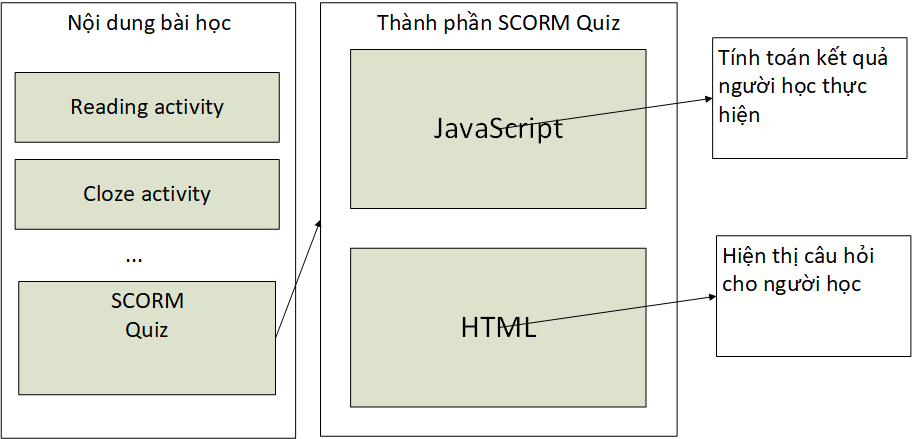
\includegraphics[width=15cm]{Chapter4/Pictures/picture41.png}
		\end{center}
		\caption{Nội dung bài học và thành phần của SCORM Quiz}
		\label{refpicture51}
	\end{figure}
\end{center}

Như vậy hình 4.1 đã cho ta thấy hạn chế của SCORM Quiz nằm ở chỗ mỗi SCORM Quiz chỉ đẩy ra được một kết quả và bộ tính toán kết quả chỉ nhận được một kết quả đưa vào. \\

\textbf{b. Cải tiến thiết kế SCORM Quiz}\\

	Để khắc phục vấn đề nêu trên, cần cải tiến mội số thiết kế của SCORM Quiz hiện tại như sau:
	\begin{itemize}
		\item Cần có một định danh duy nhất cho mỗi SCORM Quiz để các đoạn mã Javascript sau không ghi đè lên các đoạn JavaScript trước.
		
		\item Cần có một bộ tổng hợp kết quả, nhận thông tin về thiết lập của người soạn thảo rằng SCORM Quiz nào cần phải đạt.
	\end{itemize}

	\begin{center}
	\begin{figure}[htp]
		\begin{center}
			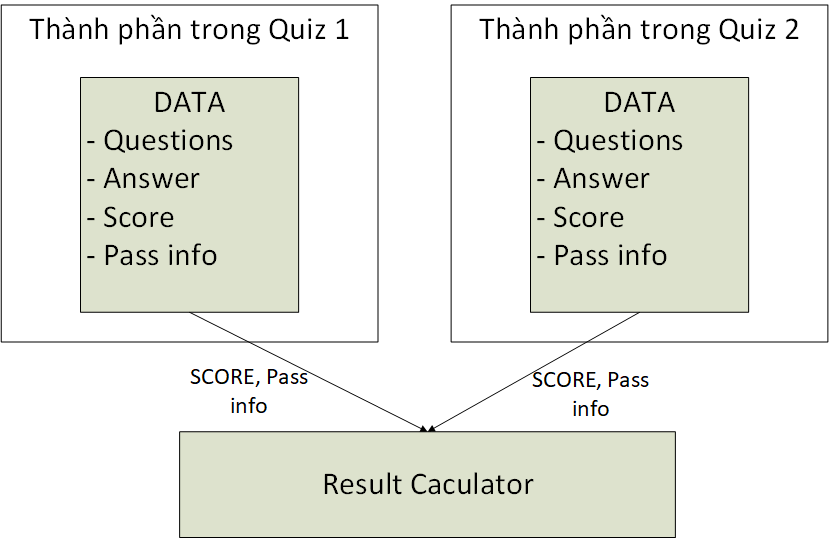
\includegraphics[width=10cm]{Chapter4/Pictures/picture42.png}
		\end{center}
		\caption{Cách cải tiến SCORM Quiz}
		\label{refpicture51}
	\end{figure}
\end{center}	

Hình 4.2 là mô hình SCORM Quiz cải tiến được đề xuất và hiện thực. Khắc phục được hạn chế về số lượng các SCORM Quiz trong một nội dung bài học như trước. Hiện thực một bộ tổng hợp kết quả gồm các toán tử logic với đầu vào là kết quả từ các SCORM Quiz có trong bài học của cây học tập và thông tin về những SCORM Quiz được người biên soạn đặt giá trị cần phải đạt, đầu ra sẽ đưa vào LMS để xử lý.

	\begin{center}
	\begin{figure}[htp]
		\begin{center}
			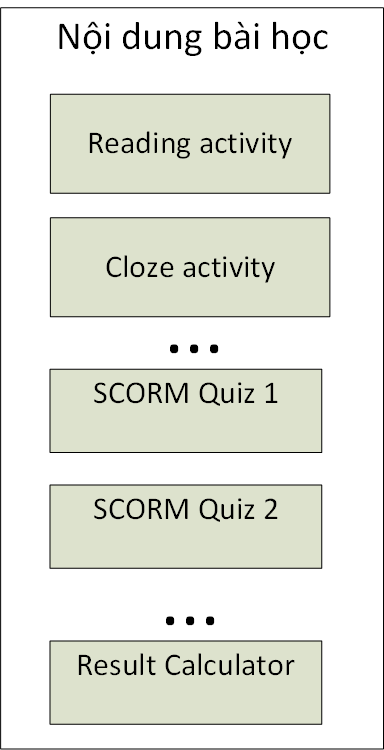
\includegraphics[width=7cm]{Chapter4/Pictures/picture43.png}
		\end{center}
		\caption{Thứ tự bộ Total score Caculator nằm trong resource file}
		\label{refpicture51}
	\end{figure}
\end{center}

	Như đã trình bày mỗi SCORM Quiz là một hoạt động được soạn thảo ra từ chức năng soạn thảo SCORM Quiz. Nội dung SCORM Quiz này sẽ bao gồm hai thành phần chính là mã Javascript để thực thi các phương thức lấy kết quả do người học lựa chọn và tính toàn điểm số, thành phần thứ hai là mã HTML để tạo ra các khung nhìn về câu hỏi cho người học thực hiện. \\
	
	Khi có nhiều SCORM Quiz được thiết kế thì sẽ có nhiều khối tương ứng được sinh ra như trong hình 4.3. Bộ tổng hợp kết quả cũng là một khối nhưng chỉ gồm một thành phần mà mã Javascript chứa các phương thức tổng hợp dành cho các SCORM Quiz. Hình 4.3 mô tả thứ tự tạo ra của các khối trong tập tin mã nguồn. Khối này sẽ được tạo ra sau SCORM Quiz cuối cùng. Như vậy LMS sẽ không nhận kết quả từ các SCORM Quiz ban đầu nữa mà chỉ nhận kết quả từ đây.\\


\subsection{Mở rộng thuộc tính cho SCORM Quiz}

	Các câu hỏi được soạn thảo trên SCORM Quiz của eXe Learning khi người biên soạn xem lại sẽ gây ra rất nhiều khó khăn. Khó khăn thứ nhất là không phân biệt được câu hỏi này thuộc phần nào trong bài học, thiếu thuộc tính phân loại về chủ đề. Khó khăn thứ hai không phân loại được độ khó của câu hỏi, thiếu thuộc tính phân loại về độ khó. Khó khăn lớn nhất là không thể tổng hợp các câu hỏi từ nhiều SCORM Quiz và tiến hành lựa chọn để tổng hợp thành một bài kiểm tra gồm nhiều mức độ và thể loại khác nhau.\\
	
	Các thuộc tính phân loại câu hỏi là cần thiết trong quá trình soạn thảo, đánh giá và tổng hợp một bài kiểm tra. Do đó, phần này sẽ đi sâu vào nghiên cứu và tìm cách khắc phục khuyết điểm này của SCORM Quiz bằng cách thêm thuộc tính phân loại vào quá trình soạn thảo.\\
	
	Về mặt thiết kế của SCORM Quiz bao gồm:
	\begin{itemize}
		\item Instructions: Các hướng dẫn sử dụng khi người biên soạn mở chức năng này.
		
		\item Question Text Area: Vùng để người biên soạn nhập câu hỏi.
		
		\item Options: Vùng nhập các câu trả lời cho câu hỏi.
		
		\item Correct Answer: Đáp án đúng của câu hỏi.
		
		\item User Answer: Đáp án người học lựa chọn.
	\end{itemize}
	
Ta sẽ thêm 3 thuộc tính về độ khó như sau: isHard, isMedium, isEasy có kiểu dữ liệu là Boolean để lưu trữ độ khó của câu hỏi này khi người soạn thảo soạn xong như hình 4.4 mô tả.	


	\begin{center}
	\begin{figure}[htp]
		\begin{center}
			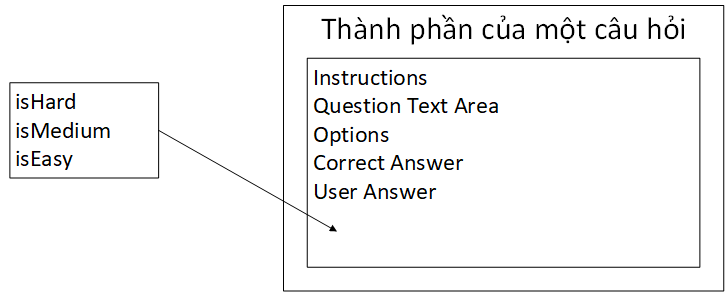
\includegraphics[width=15cm]{Chapter4/Pictures/picture44.png}
		\end{center}
		\caption{Thêm ba thuộc tính phân loại vào các các thành phần của một câu hỏi}
		\label{refpicture51}
	\end{figure}
\end{center}

Về mặt hiển thị đối với người biên soạn. Ba thuộc tính trên sẽ được biểu diễn bằng nhóm các đối tượng radio button. Bao gồm 3 radio button Hard (Khó), Medium (Trung bình) và Easy (Dễ) như hình 4.5 mô tả.

\newpage
	\begin{center}
	\begin{figure}[htp]
		\begin{center}
			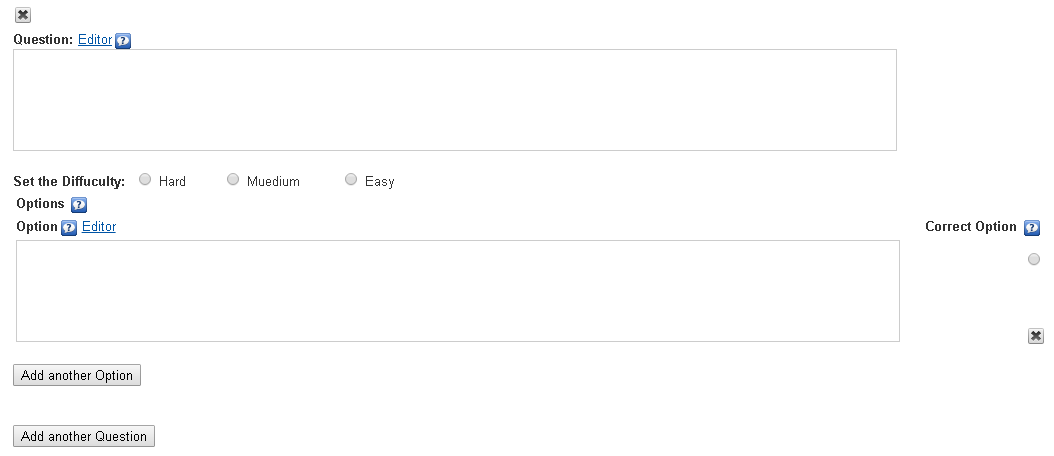
\includegraphics[width=15cm]{Chapter4/Pictures/picture45.png}
		\end{center}
		\caption{Giao diện soạn thảo câu hỏi}
		\label{refpicture51}
	\end{figure}
\end{center}


	Thuộc tính độ khó này đóng vai trò rất quan trọng trong quá trình soạn thảo bài học. Thuộc tính phân loại giúp người soạn thảo đánh giá được mức độ của bài học. Kiểm soát được mức độ của bài học cũng như mức độ của SCORM Quiz. Các thuộc tính độ khó này chỉ xuất hiện ở khung nhìn của người soạn thảo như hình 4.6, người học sẽ không thấy được thuộc tính này, có nghĩa là người học sẽ không biết được câu hỏi mình đang thực hiện có độ khó như thế nào.
	
	
	\begin{center}
		\begin{figure}[htp]
			\begin{center}
			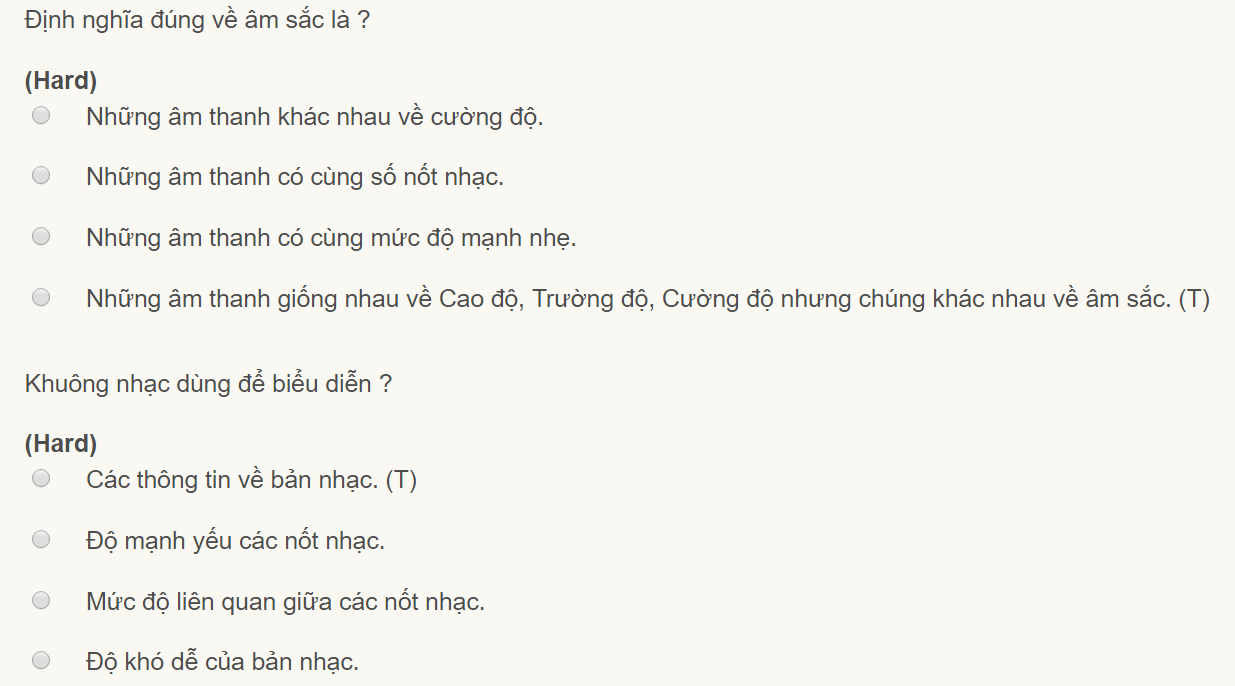
\includegraphics[width=15cm]{Chapter4/Pictures/picture46.png}
			\end{center}
			\caption{Ví dụ một khung nhìn của người soạn thảo}
			\label{refpicture52}
		\end{figure}
	\end{center}	

	\newpage
		
	\subsection{Chức năng tổng hợp câu hỏi và tạo bài kiểm tra}
	\textbf{a.	Tổng hợp câu hỏi}\\
	
		Soạn thảo câu hỏi, đánh giá người học dựa trên các câu hỏi của một SCORM Quiz không thì vẫn chưa đủ. Vì mỗi SCORM Quiz thường được biên soạn với mục đích ôn tập kiến thức là chủ yếu. Mỗi SCORM Quiz thường xoay quanh một chủ đề nhất định, không bao quát được tất cả vấn đề trong bài học. SCORM Quiz thường có số lượng câu hỏi ít từ năm đến mười câu hỏi, vì nếu soạn thảo nhiều câu hỏi trên giao diện soạn thảo của SCORM Quiz sẽ rất khó khăn do độ trễ của mỗi thao tác càng lúc càng lớn.\\
		
		Do thiết kế cứng nhắc ban đầu của SCORM Quiz nên nội dung các câu hỏi của SCORM Quiz được tạo cho người học thực hiện là cố định, không có sự thay đổi của số câu hỏi cũng như vị trí câu hỏi và câu trả lời. Hình 4.7 là mô tả việc xuất nội dung của SCORM Quiz thành resource file. Resource file này sẽ gồm hai phần chính là mã Javascript ghi nhận các câu trả lời mà người học chọn và tính điểm, phần câu hỏi và các lựa chọn trả lời sẽ được hiển thị dưới dạng HTML cứng không thay đổi được với các lần truy cập khác nhau, dẫn đến việc không khách quan nếu như người học làm lại lần thứ hai, lần thứ ba,...\\
	
	\begin{center}
	\begin{figure}[htp]
		\begin{center}
			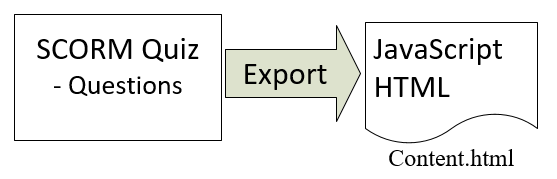
\includegraphics[width=10cm]{Chapter4/Pictures/picture47.png}
		\end{center}
		\caption{SCORM Quiz xuất nội dung thành Resource File}
		\label{refpicture55}
	\end{figure}
\end{center}
	
	Để khắc phục các hạn chế trên, nhóm đề xuất hiện thực một chức năng soạn thảo, tổng hợp câu hỏi từ nhiều SCORM Quiz dựa trên độ khó của mỗi câu hỏi. Các câu hỏi được tạo cho người học sẽ thay đổi được vị trí cũng như vị trí câu trả lời trong từng câu hỏi. Chức năng này được thiết kế thành một công cụ kiểm tra riêng biệt với tên SCORM Test.\\
	
	SCORM Test là một chức năng sẽ được xây dựng sẵn trong hệ thống eXe Learning. Được lưu trữ trong iDevice Store cùng với các iDevice khác. iDevice Store này sẽ được lưu trữ Local trong thiết bị. Được thiết kế như là một chức năng soạn thảo câu hỏi tương tự như SCORM Quiz nhưng đi kèm một số tính năng vượt trội hơn.\\
	
	iDevice này sẽ có 3 chế độ hoạt động khác nhau. Edit Mode, Author View Mode và Learner View Mode. Edit Mode là chế độ soạn thảo cho người biên soạn. Author View Mode là chế độ xem dành cho người soạn thảo, giống như SCORM Quiz, soạn thảo xong sẽ chuyển sang chế độ này. Learner View Mode là chế độ xem dành cho người học, khác với Author View Mode, chế độ xem này chỉ có những câu hỏi nào người biên soạn chọn mới được đưa ra ở đây.

	\begin{center}
	\begin{figure}[htp]
		\begin{center}
			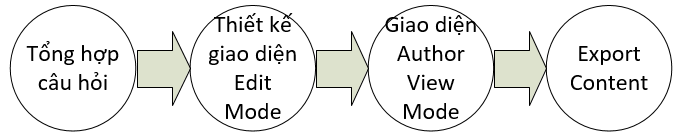
\includegraphics[width=10cm]{Chapter4/Pictures/picture48.png}
		\end{center}
		\caption{Quy trình hiện thực công cụ kiểm tra SCORM Test}
		\label{refpicture56}
	\end{figure}
\end{center}

	
\newpage

	Hình 4.8 là mô tả quá trình nhóm hiện thực iDevice. Bước đầu là việc thiết kế giao diện tổng hợp các câu hỏi từ các SCORM Quiz. Thiết kế bộ Selector để cho người biên soạn lựa chọn câu hỏi xuất hiện trong bài kiểm tra. Tiếp theo là thiết kế giao diện hiển thị cho người soạn thảo, giao diện này sẽ khác so với giao diện làm câu hỏi của người học. Cuối cùng là hiện thực phần xuất các thành phần của iDevice  thành Resource file. Resource file này phải khắc phục được các hạn chế của SCORM Quiz trình bày ra ở hình 4.1, phải đảm bảo sao cho các câu hỏi mỗi lần thực hiện trên SCORM Cloud phải là động.\\
	
		
	\textbf{b. Hiện thực việc thiết kế iDevice}\\
	
	SCORM Test là iDevice dùng cho việc soạn thảo và tổng hợp. Do đó, có tích hợp cả tính năng soạn thảo câu hỏi của SCORM Quiz vào, người dùng có thể sử dụng SCORM Test để soạn thảo câu hỏi. Tuy nhiên nhiệm vụ và chức năng chính của SCORM Test là tổng hợp câu hỏi và lựa chọn câu hỏi từ nhiều SCORM Quiz khác nhau. \\
	
	Từ hình 4.8 mô tả trên, nhóm đã nghiên cứu và đưa ra mô hình thiết kế tổng quan của SCORM Test như sau:
	
	\begin{center}
	\begin{figure}[htp]
		\begin{center}
			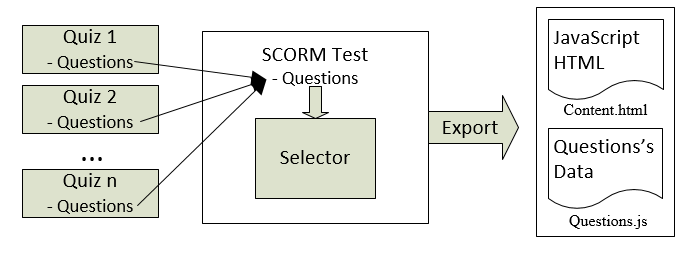
\includegraphics[width=16cm]{Chapter4/Pictures/picture49.png}
		\end{center}
		\caption{Tổ chức của SCORM Test}
		\label{refpicture57}
	\end{figure}
\end{center}

	Hình 4.9 là tổ chức của SCORM Test do nhóm đề xuất hiện thực. Mô hình này có thể khắc phục được hạn chế trong quá trình Export của SCORM Quiz. Cụ thể tất cả các bước hiện thực được đưa ra ở hình 4.9. Các bước thực gồm bốn phần được trình bày như sau.\\
	
	Phần thứ nhất, chức năng tổng hợp của SCORM Test được thực hiện như sau. Khi người dùng chọn iDevice SCORM Test, sẽ thực hiện một quá trình duyệt đệ quy trên tất các các bài học của cây học tập, quá trình này sẽ thu thập tất cả các câu hỏi từ những SCORM Quiz đã biên soạn trước được tổng hợp vào danh sách câu hỏi của SCORM Test này và hiển thị dưới dạng Edit mode cho người biên soạn chỉnh sửa. \\
	
	Phần thứ hai, chức năng lựa chọn câu hỏi được thực hiện như sau. Sau khi quá trình tổng hợp hoàn tất, sẽ xuất hiện một bộ Selector ở dưới phần câu hỏi. Bộ Selector này sẽ gồm ba trường nhập vào cho mỗi SCORM Quiz tương ứng với ba mức độ câu hỏi khó, trung bình và dễ. Người biên soạn sẽ nhập vào số lượng câu hỏi tương ứng.

\newpage

	\begin{center}
	\begin{figure}[htp]
		\begin{center}
			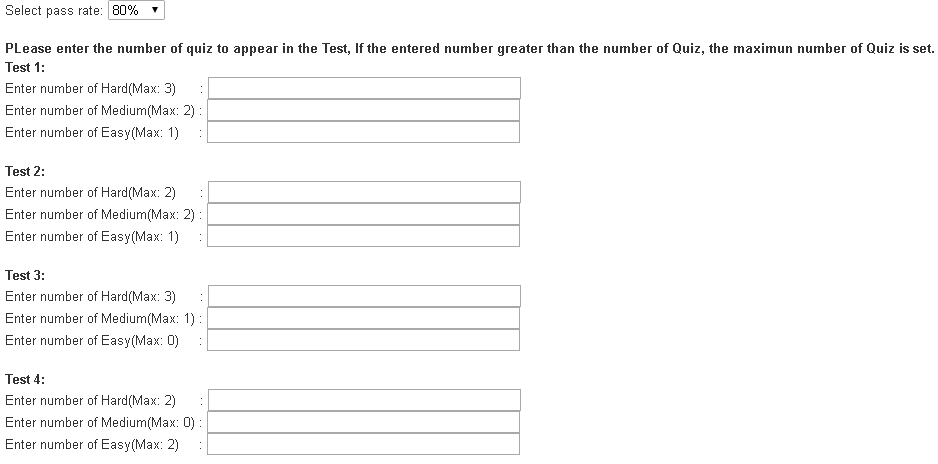
\includegraphics[width=16cm]{Chapter4/Pictures/picture410.png}
		\end{center}
		\caption{Chế độ Edit Mode của SCORM Test}
		\label{refpicture58}
	\end{figure}
\end{center}

Hình 4.10 là giao diện cho bộ cấu hình bài kiểm tra của SCORM Test. Người soạn thảo sẽ lựa chọn tỷ lệ đạt (Pass Rate) cho bài kiểm tra và chọn các câu hỏi sẽ được hiển thị lên bài kiểm tra. Số câu hỏi tối đa của từng độ khó cũng sẽ được thống kê ở đây, nếu người dùng nhập vào số lượng câu hỏi nhiều hơn số câu hỏi tối đa thì số câu hỏi tối đa sẽ được chọn.\\

	\begin{center}
	\begin{figure}[htp]
		\begin{center}
			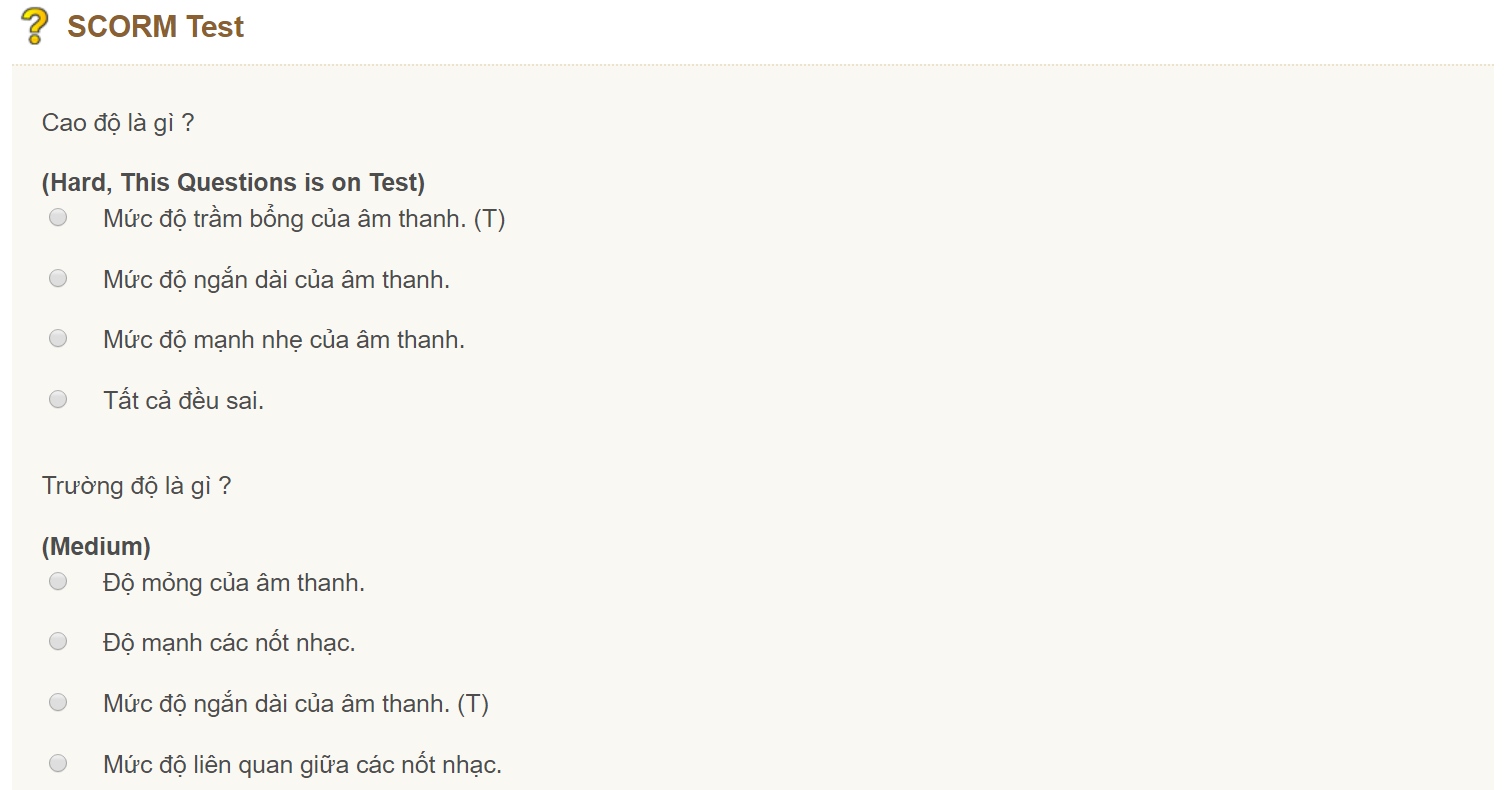
\includegraphics[width=16cm]{Chapter4/Pictures/picture411.png}
		\end{center}
		\caption{SCORM Test ở chế độ Author View Mode}
		\label{refpicture58}
	\end{figure}
\end{center}

\newpage

	Phần thứ ba, sau khi người soạn thảo cấu hình xong sẽ chuyển sang View mode dành cho người biên soạn. Người biên soạn có thể theo dõi được tất cả các câu hỏi có trong bài học. Hình 4.11 là giao diện Author View Mode. Các câu hỏi sẽ được gắn hai nhãn đánh dấu, nhãn thứ nhất đánh dấu về độ khó của câu hỏi, nhãn thứ hai đánh dấu cho biết câu hỏi nào sẽ được xuất hiện trong bài kiểm tra.\\
	
	Phần thứ tư là xuất các nội dung đã được thiết lập trong quá trình soạn thảo SCORM Test thành các Resource File. Đây là bước khó nhất trong toàn bộ quá trình đã đưa ra ở hình 4.9, phải nghiên cứu và khắc phục được mô hình Export cứng nhắc của SCORM Quiz. Nhóm đề xuất một quá trình Export thành hai file khác nhau, Một file data chứa nội dung các câu hỏi và trả lời tương ứng định với dịnh dạng file Javascript. File thứ hai là file chứa nội dung của bài học theo định dạng file HTML. \\
	
	File nội dung định dạng HTML này sẽ gồm hai phần, phần đầu sẽ là mã JavaScript, phần thứ 2 là mã HTML chứa nội dung được hiển thị ra. Nguyên tắc xử lý sẽ được trình bày như sau.\\
	
		\begin{center}
		\begin{figure}[htp]
			\begin{center}
				\includegraphics[width=15cm]{Chapter4/Pictures/picture412.png}
			\end{center}
			\caption{Công việc của mả Javascript trong file content.html}
			\label{refpicture510}
		\end{figure}
	\end{center}


Hình 4.12 mô tả quá trình hiện thực mã Javascript trong file content.html. Bước thứ nhất sẽ xây dựng một cấu trúc dữ liệu thích hợp dùng để lưu trữ câu hỏi, một câu hỏi sẽ có các thuộc tính được định nghĩa như bảng 4.1 ở dưới.\\

\begin{table}[!htp]
	\centering
	\begin{tabular}{|l|c|l|}
		\hline 
		\textbf{Name} 	& \textbf{Data Type} 	& \hspace{2.6cm}\textbf{Ý nghĩa} \\ 
		\hline 
		Id 				& String 				& Định danh duy nhất cho từng câu hỏi.\\ 
		\hline 
		Text 			& String 				& Phần nội dung câu hỏi.\\ 
		\hline 
		Answers 		& Array 				& Mảng chứa các câu trả lời tương ứng.\\ 
		\hline 
		CorrectAnswer	& String 				& Câu trả lời đúng.\\ 
		\hline
		ObjectID 		& String 				& Cho biết câu hỏi này thuộc Object nào.\\  
		\hline
	\end{tabular}
	\caption{Các thuộc tính của một câu hỏi}
	\label{reftable51}
\end{table}

%Bước thứ hai sẽ nhận input là data từ file questions.js để đọc và lưu trữ thành một mảng các Questions Object. File questions.js là phần đầu của Resource File như đã trình bày ở trên. Mảng các Questions Object là mảng chứa các câu hỏi đã lưu trữ, với mục đích tạo bài kiểm tra.\\

Bước thứ hai, sẽ nhận input là data từ file questions.js để đọc và lưu trữ thành một mảng các Questions Object.\\

		\begin{center}
	\begin{figure}[htp]
		\begin{center}
			\includegraphics[width=15cm]{Chapter4/Pictures/picture413.png}
		\end{center}
		\caption{Đoạn mã Javascript sắp xếp lại các câu hỏi ở mỗi lần tạo}
		\label{refpicture510}
	\end{figure}
\end{center}

Bước thứ ba là xây dựng các phương thức sinh bài kiểm tra với khung nhìn của người học từ mảng câu hỏi đã được lưu trữ. Mỗi lần tạo sẽ thực hiện việc sắp xếp lại thứ tự các câu hỏi trong mảng bằng cách sử dụng hàm sort có sẵn trong Javascript, hình 4.13 mô tả đoạn mã này, với mục đích đảm bảo rằng các câu hỏi ở mỗi lần hiển thị đều sẽ ở các vị trí khác nhau.



\subsubsection{c. Kết quả}

Kiểm tra kết quả sau khi hiện thực được tiến hành như sau. Sau khi hiện thực thành công chức năng, tiến hành đóng gói nội dung với nhiều SCORM Quiz, ở bài học cuối cùng ta dùng tính năng SCORM Test để tổng hợp câu hỏi, đóng gói nội dung lại và upload lên SCORM Cloud để kiểm tra kết quả. Hình 4.14 là giao diện khóa học khi upload nội dung lên SCORM Cloud.

	\begin{center}
		\begin{figure}[htp]
			\begin{center}
				\includegraphics[width=9cm]{Chapter4/Pictures/picture414.png}
			\end{center}
			\caption{Course menu với SCORM Test}
			\label{refpicture511}
		\end{figure}
	\end{center}

Hình 4.15 mô tả quá trình hai lần thực hiện SCORM Test. Ta có thể thấy các câu hỏi cũng như các câu trả lời tương ứng đã có thể thay đổi được vị trí khi thực hiện nhiều lần khác nhau.

	\begin{center}
		\begin{figure}[htp]
			\begin{center}
				\includegraphics[width=10cm]{Chapter4/Pictures/picture415.png}
			\end{center}
			\caption{Sinh đề kiểm tra với SCORM Test }
			\label{refpicture512}
		\end{figure}
	\end{center}








\chapter{KIỂM THỬ PHẦN MỀM}
\begin{flushleft}
	\fontsize{12pt}{7pt}\selectfont
	\textit{Chương này sẽ trình bày về quá trình kiểm thử phần mềm cho eXe. Mục đầu tiên sẽ trình bày về chiến lược kiểm thử cùng các giai đoạn kiểm thử. Mục tiếp theo sẽ nêu ra các thử thách trong quá trình kiểm thử, bao gồm thử thách về mặt công nghệ và sự bùng nổ về số lượng mẫu kiểm tra. Mục thứ ba sẽ đưa ra các hướng giải quyết cho các thử thách này và mục cuối cùng là ví dụ một mẫu kiểm tra đã hiện thực.}
\end{flushleft}

\section{Chiến lược kiểm thử}

Selenium Webdriver là công cụ kiểm thử tự động được lựa chọn để kiểm thử cho eXe. Lý do là cả eXe và SCORM Cloud đều được sử dụng trên trình duyệt. Selenium Webdriver có khả năng tương tác rất tốt với mọi đối tượng trên trình duyệt, vì vậy sẽ rất thích hợp để kiểm thử cho toàn bộ quá trình thực hiện.\\

Để sử dụng một bài giảng điện tử cần một quá trình có hai công việc. Công việc thứ nhất là người soạn thảo sẽ sử dụng eXe để soạn thảo bài giảng, thiết kế nội dung cho các bài học, thiết lập các điều kiện cần thiết cho mỗi bài học,... cuối cùng là đóng gói bài giảng theo chuẩn SCORM 2004 và upload lên SCORM Cloud. Công việc thứ hai là người học thực hiện các bài học có trong bài giảng và hoàn thành tất cả bài học này. Toàn bộ quá trình này đều được tự động hóa bằng Selenium Webdriver.\\

Chiến lược kiểm thử sẽ là quá trình kiểm thử tích hợp (Integration Testing) nhằm mục đích mô phỏng toàn bộ quá trình hoạt động để xây dựng và sử dụng một bài giảng điện tử. Đầu tiên Selenium Webdriver sẽ đóng vai trò người soạn thảo, tự động hóa các công việc như soạn thảo bài giảng, thiết kế nội dung cho các bài học, thiết lập các điều kiện cần thiết cho mỗi bài học,... cuối cùng là đóng gói bài giảng theo chuẩn SCORM 2004 và upload khóa học lên SCORM Cloud. Tiếp theo Selenium Webdriver sẽ đóng vai trò người học, tự động hóa việc tham gia vào bài học và hoàn thành các bài học.\\

Mục đích của chiến lược kiểm thử là đảm bảo cho bài giảng điện tử được tạo ra đúng như thiết lập của người soạn thảo. Đầu tiên người soạn thảo sẽ sử dụng eXe để soạn thảo bài giảng, thiết kế nội dung cho các bài học, thiết lập các điều kiện cần thiết cho mỗi bài học,... cuối cùng là đóng gói bài giảng theo chuẩn SCORM 2004, lúc này bài giảng ngoài nội dung còn có các mã SCORM được sinh ra theo như các thiết lập điều kiện của người soạn thảo. Tiếp theo người soạn thảo sẽ upload bài giảng lên SCORM Cloud, lúc này sẽ kiểm tra cho việc mã SCORM có chạy đúng như đã sinh ra hay không.

\newpage

\begin{center}
	\begin{figure}[htp]
		\begin{center}
			\includegraphics[width=5cm]{Chapter5/Pictures/picture51.png}
		\end{center}
		\caption{Toàn bộ quá trình kiểm thử}
		\label{refhinhchuong71}
	\end{figure}
\end{center}

Hình 5.1 mô tả toàn bộ quá trình kiểm thử tự động. Selenium Webdriver sẽ tự động hóa sử dụng eXe để soạn thảo bài giảng, thiết kế nội dung bài giảng, thiết lập các điều kiện cần thiết cho mỗi bài học, đóng gói bài giảng theo chuẩn SCORM 2004, tiếp theo sẽ upload bài giảng lên SCORM Cloud và tự động tham gia, hoàn thành bài học.
\newpage

\section{Các thử thách trong quá trình kiểm thử}
\subsection{Thử thách về mặt công nghệ}

Thách thức đầu tiên là về mặt thiết kế của eXe. Vì được thiết kế giao diện bằng ExtJS nên eXe sinh ra các đối tượng động. Các đối tượng động ở đây có thể là id, class, button,... hoặc có thể là bất kỳ cặp thẻ HTML nào. eXe còn tự động sinh ra các frame ngẫu nhiên, khiến các đối tượng bị ẩn đi. Những điều này dẫn đến việc xác định các thành phần của eXe rất khó khăn. \\

Thách thức thứ hai là áp dụng kiểm thử tự động cho eXe. Để kiểm thử tự động hiệu quả, chúng ta cần xác định được các thành phần của eXe, tuy nhiên do eXe sinh ra các đối tượng động như trình bày ở trên nên việc này trở nên khó khăn. ExtJS tạo ra những phần tử có cấu trúc phức tạp, có số lượng lớn id hoặc class trùng lặp với nhau. Việc xử lý vấn đề này sẽ được trình bày ở chương sau.\\


\subsection{Thử thách về số lượng mẫu kiểm tra}

Bùng nổ về số lượng mẫu kiểm tra là một vấn đề hết sức phổ biến trong kiểm thử phần mềm. Đa số các phần mềm đều cần có một số lượng mẫu kiểm tra rất lớn để kiểm thử các tính năng của chúng, eXe cũng không phải ngoại lệ và cần phải tìm cách để giảm số lượng mẫu kiểm tra xuống một cách hợp lý.


\begin{comment}
Đối với hướng phát triển thứ nhất, việc kiểm thử bao gồm 2 giai đoạn. Giai đoạn thứ nhất là thiết lập tiền điều kiện (PreCondition) cho mỗi bài học, đây là điều kiện để người học có thể học bài này. Giai đoạn thứ hai là thiết lập hậu điều kiện (PostCondition) cho mỗi bài học, đây là điều kiện để xác định người học hoàn thành bài học này.\\

Giai đoạn thứ nhất là thiết lập tiền điều kiện, chúng ta cần thiết lập thứ tự các bài học để người học tham gia đầy đủ toàn bộ các bài. Sau đây là cách tính các trường hợp có thể xảy ra cho giai đoạn thứ nhất:

\begin{itemize}
\item Một khóa học bao gồm nhiều bài học. Người học cần phải tham gia đầy đủ các bài học thì mới được xem là hoàn thành khóa học.

\item Lấy ví dụ 1 khóa học có 3 bài học, như vậy ta sẽ có 3! = 6 cách thiết lập thứ tự các bài để người học tham gia đầy đủ 3 bài học. Cách thiết lập thứ nhất là người học có thể học bài 1, sau đó đến bài 2 và cuối cùng là bài 3. Cách thiết lập thứ 2 là người học có thể bắt đầu từ bài 2, sau đó học bài 1 và cuối cùng là bài 3,...

\item Một cách tổng quát, đối với 1 khóa học có n bài học thì sẽ có n! cách thiết lập thứ tự các bài để người học hoàn thành khóa học.

\end{itemize}

Như vậy giai đoạn thứ nhất sẽ có số lượng testcase là n!.\\

Giai đoạn thứ hai là thiết lập hậu điều kiện cho mỗi bài học, cần thiết lập điều kiện để xác định người học đã hoàn thành bài học. Có 2 trường hợp được xem là hoàn thành bài học. Trường hợp thứ nhất là người học cần phải ở bài học trong 1 khoảng thời giai nhất định, phải học ở bài học trong khoảng thời giai đã thiết lập thì mới được xem là hoàn thành bài này. Trường hợp thứ hai là phải vượt qua những bài kiểm tra ở bài này, người học cần phải đạt những bài kiểm tra đã quy định thì mới được xem là hoàn thành bài học. Sau đây là cách tính các trường hợp có thể xảy ra cho giai đoạn thứ hai:

\begin{itemize}
\item Trường hợp thứ nhất là phải ở bài học trong khoảng thời giai đã quy định. Đối với trường hợp này chỉ có 2 trường hợp là có thời giai hoặc không có thời giai ở mỗi bài. Như vậy một cách tổng quát, đối với 1 khóa học có n bài học thì sẽ có tổng cộng 2n testcase cho trường hợp này.

\item Trường hợp thứ hai là phải vượt qua những bài kiểm tra đã quy định thì mới được xem là hoàn thành bài học.Có 2 cách thiết lập chính cho trường hợp này. Cách thứ nhất là thiết lập chính xác các bài kiểm tra cần đạt. Cách thứ hai là thiết lập chỉ cần đạt một bài kiểm tra bất kỳ trong các bài kiểm tra này. Sau đây là cách tính cho trường hợp này:
\begin{itemize}
\item Lấy ví dụ một bài học có 3 bài kiểm tra, với cách thứ nhất là cần đạt những bài kiểm tra đã thiết lập, chúng ta có những trường hợp sau đây:

\begin{itemize}
\item Nếu thiết lập cần đạt 1 bài kiểm tra trong 3 bài này thì sẽ có tổ hợp 1 trong 3 bài này, tức $C_3^1$ = 3 cách thiết lập. Cách thiết lập thứ nhất là đạt bài 1, cách thiết lập thứ 2 là đạt bài 2 và cách thiết lập thứ 3 là đạt bài 3. Một cách tổng quát, để thiết lập cần đạt 1 bài kiểm tra trong m bài kiểm tra thì trong trường hợp này sẽ có $C_m^1$ cách thiết lập.

\item Nếu thiết lập cần đạt 2 bài kiểm tra trong 3 bài này thì sẽ có tổ hợp 2 trong 3 bài này, tức $C_3^2$ = 3 cách thiết lập. Cách thiết lập thứ nhất là cần đạt bài 1 và bài 2, cách thiết lập thứ hai là cần đạt bài 2 và bài 3 và cách thiết lập thứ ba là cần đạt bài 1 và bài 3. Một cách tổng quát, để thiết lập cần đạt 2 bài kiểm tra trong m bài kiểm tra thì trong trường hợp này sẽ có $C_m^2$ cách thiết lập.

\item Như vậy công thức tổng quát cho trường hợp này là $C_m^1 + C_m^2 + C_m^3 + ... + C_m^{m-1} + C_m^m$, với $m\in\mathbb{N^*}$. Trong đó m là tổng số bài kiểm tra trong một bài học.


\end{itemize}

\item Lấy ví dụ một bài học có 3 bài kiểm tra, với cách thứ hai là chỉ cần đạt một bài kiểm tra bất kỳ trong các bài kiểm tra này, chúng ta có những trường hợp sau đây:
\begin{itemize}
\item Lấy ví dụ 1 bài học có 3 kiểm tra, sẽ có tổ hợp 1 trong 3 bài này, tức $C_3^1$ = 3 testcase. Testcase thứ nhất để kiếm tra là sau khi đạt bài 1 thì có được xem là hoàn thành bài học hay không, testcase thứ hai để kiếm tra là sau khi đạt bài 2 thì có được xem là hoàn thành bài học hay không và testcase thứ ba để kiếm tra là sau khi đạt bài 3 thì có được xem là hoàn thành bài học hay không. 

\item Một cách tổng quát, để kiểm tra cần đạt 1 bài kiểm tra bất kỳ trong m bài kiểm tra thì trong trường hợp này sẽ có $C_m^1$ testcase, với $m\in\mathbb{N^*}$. Trong đó m là tổng số bài kiểm tra trong một bài học.
\end{itemize}


\item Tổng quát cho trường hợp thứ hai là phải vượt qua những bài kiểm tra đã quy định thì mới được xem là hoàn thành bài học, sẽ có công thức tổng quát là $n*(C_m^1 + C_m^2 + C_m^3 + ... + C_m^{m-1} + C_m^m) + n*C_m^1$, với $m,n\in\mathbb{N^*}$, trong đó n là tổng số bài học trong khóa học, m là tổng số bài kiểm tra trong mỗi bài.

\end{itemize}



\end{itemize}

Như vậy tổng kết cho giai đoạn thứ hai sẽ có số lượng testcase là $2n + n*(C_m^1 + C_m^2 + C_m^3 + ... + C_m^{m-1} + C_m^m) + n*C_m^1$, với $m,n\in\mathbb{N^*}$, trong đó n là tổng số bài học trong khóa học, m là tổng số bài kiểm tra trong mỗi bài.\\


Như vậy số lượng testcase tổng cộng cho hướng phát triển thứ nhất là $n! * (2n + n*(C_m^1 + C_m^2 + C_m^3 + ... + C_m^{m-1} + C_m^m) + n*C_m^1)$, với $m,n\in\mathbb{N^*}$, trong đó n là tổng số bài học trong khóa học, m là tổng số bài kiểm tra trong mỗi bài.\\

Với công thức trên, ví dụ một khóa học có 5 bài học, mỗi bài học có 3 bài kiểm tra thì số lượng testcase sẽ là $5! * (2*5 + 5*(C_3^1 + C_3^2 + C_3^3) + 5*C_3^1) = 7200$ testcase. Đây là một con số quá lớn, do đó chúng ta cần có những phương pháp biện luận để có thể giảm số lượng testcase này.
\end{comment}	

Mỗi bài học đều có tiền điều kiện và hậu điều kiện. Tiền điều kiện là điều kiện mà người học cần thỏa mãn để được vào học một bài học, tiền điều kiện của 1 bài học là bài học mà người học cần phải hoàn thành (thỏa mãn hậu điều kiện) trước khi vào nội dung bài học này. Hậu điều kiện là điều kiện xác nhận người học đã hoàn thành bài học này, hậu điều kiện có thể là thời gian tối thiểu người học phải bỏ ra cho một bài học hoặc phải đạt một số bài kiểm tra nào đó do người biên soạn quy định. Để đảm bảo người học tiếp thu đầy đủ kiến thức ở tất cả các bài, mỗi bài học phải được người học tham gia ít nhất một lần. Một khóa học bao gồm nhiều bài học. Người học cần phải tham gia đầy đủ các bài học thì mới được xem là hoàn thành khóa học.\\

Công việc đầu tiên là thiết lập tiền điều kiện cho mỗi bài học. Mỗi bài học đều có thể có tiền điều kiện là bài học trước của nó, tức một bài học ở vị trí thứ $X$ có thể có tiền điều kiện là bài học có vị trí thứ $X-1$. Như vậy đối với một khóa học có $n$ bài học thì số tiền điều kiện có thể xảy ra là $n!$.\\

Công việc thứ hai là thiết lập hậu điều kiện cho mỗi bài học. Hậu điều kiện có thể là thời gian người học cần phải bỏ ra hoặc đạt các bài kiểm tra theo quy định của người soạn thảo. Lấy ví dụ mỗi bài học đều có 3 bài kiểm tra, như vậy ta sẽ có các cách thiết lập như tại mỗi bài đều có thời gian, phải đạt bài kiểm tra thứ 1, phải đạt bài kiểm tra thứ hai, đạt bài kiểm tra thứ 3, đạt hai bài kiểm tra thứ nhất và thứ hai,... hoặc đạt cả ba bài kiểm tra. Như vậy trong ví dụ này ta có tổng cộng 9 cách thiết lập hậu điều kiện ở mỗi bài.\\

Như vậy đối với một khóa học có $n$ bài học, ở mỗi bài học có ba bài kiểm tra thì số mẫu kiểm tra sẽ là \textbf{$n! * 9^n$}. Lấy trường hợp 1 khóa học có 5 bài học thì số lượng mẫu kiểm tra là $7.085.880$, số lượng này là quá lớn, cần phải tìm cách để giảm bớt số lượng mẫu kiểm tra và hướng giải quyết sẽ được trình bày trong phần tiếp theo.\\



\section{Các hướng giải quyết cho quá trình kiểm thử}


\subsection{Giải quyết về mặt công nghệ}

Về cơ bản, Selenium Webdriver tác động lên các phần tử của trang web. Các phần tử đó có thể là id, class, button,... hoặc có thể là bất kỳ cặp thẻ html nào. Bộ thư viện của Selenium Webdriver cho phép chúng ta tương tác với mọi cặp thẻ html trong trang web.\\

Đối với các trang web hoặc ứng dụng web thông thường, điều này rất dễ dàng. Do tất cả các thành phần trong trang web đó đều cố định, tức id, class, button,... đều dễ dàng xác định.\\

Tuy nhiên, việc xác định các thành phần của eXe cần những phương pháp phức tạp hơn. Vì eXe được thiết kế giao diện bằng ExtJS, việc định vị các phần tử trong các ứng dụng viết bằng ExtJS là một việc rất khó khăn vì ExtJS tạo ra một trong những cấu trúc DOM phức tạp, có id động với một số lượng lớn các class trùng lặp.\\

\begin{center}
	\begin{figure}[htp]
		\begin{center}
			\includegraphics[width=15cm]{Chapter5/Pictures/picture52.png}
		\end{center}
		\caption{Đoạn mã HTML thể hiện Button Add Page của eXe}
		\label{refhinhchuong711}
	\end{figure}
\end{center}

Hình 5.2 ở trên thể hiện button Add Page của eXe, chúng ta có thể thấy ID của nó là button-2521-btnWrap, đây là 1 ID động và rất khó khăn để có thể xác định chính xác, vì mỗi lần chạy eXe, nó lại sinh ra 1 ID khác.\\

Để xử lý vấn đề này, chúng ta cần có những phương pháp phức tạp hơn. Trong luận văn này trình bày 2 phương pháp sau đây.

\begin{center}
	\begin{figure}[htp]
		\begin{center}
			\includegraphics[width=15cm]{Chapter5/Pictures/picture53.png}
		\end{center}
		\caption{Đoạn mã Python thể hiện cách xác định một phần tử có 2 thuộc tính}
		\label{refhinhchuong65}
	\end{figure}
\end{center}

Phương pháp thứ nhất là xác định phần tử bằng nhiều thuộc tính cùng 1 lúc. Hình 5.3 ở trên thể hiện cách xác định 1 phần tử có thuộc tính thứ nhất là thẻ div có \textbf{id=’footer’}, thuộc tính thứ hai là thẻ div có class là \textbf{‘x-grid3-body’}. Phương pháp này đòi hỏi phải biết chính xác các thuộc tính mà phần tử đó có và quan trọng nó phải là duy nhất so với các phần tử còn lại.\\

\begin{center}
	\begin{figure}[htp]
		\begin{center}
			\includegraphics[width=15cm]{Chapter5/Pictures/picture54.png}
		\end{center}
		\caption{Đoạn mã Python thể hiện cách dùng thuộc tính text để xác định một phần tử}
		\label{refhinhchuong66}
	\end{figure}
\end{center}

Phương pháp thứ hai là dựa vào một thuộc tính riêng của một phần tử. Hình 5.4 ở trên thể hiện cách xác định 1 phần tử có thuộc tính \textbf{text} là \textbf{‘Free Text’}, vì có rất nhiều phần tử có chung thuộc tính là \textbf{class = ‘x-grid-cell-inner’}, do đó sẽ cho tất cả phần tử này vào cùng 1 danh sách (List), sau đó sẽ duyệt từng phần tử trong List này, nếu phần tử nào có thuộc tính là \textbf{text = ‘Free Text’} thì chúng ta sẽ chọn. Phương pháp này giúp chúng ta xác định mọi loại phần tử, tuy nhiên sẽ gây chậm nếu có quá nhiều phần tử có chung một thuộc tính. Do đó cần cân nhắc giữa hai phương pháp để xác định các phần tử hiệu quả nhất.

\newpage 

\subsection{Giải quyết về thiết kế số lượng mẫu kiểm tra}


Trong phần thách thức đã nêu ở trên, nếu một khóa học có n bài học thì sẽ có $n! * 9^n$ cách sắp xếp thứ tự các bài trong khóa học này. Con số này là quá lớn, cần có những phương pháp lập luận để giảm số lượng testcase xuống ít hơn.\\

Thông thường người soạn thảo thiết kế một khóa học có 5 bài học. Vì vậy lúc này số lượng tiền điều kiện xảy ra sẽ là $5!$. Tuy nhiên để đảm bảo về mặt chuyên môn, cần có những thiết kế khác để đảm bảo chất lượng của khóa học, không phải bài học nào cũng cần phải thay đổi vị trí với nhau. Thông thường "Bài 1" sẽ là bài để mở đầu khóa học, giới thiệu chung về khóa học nên vị trí của nó sẽ luôn là đầu tiên trong khóa học và "Bài 5" sẽ là bài tổng kết của khóa học, do đó vị trí của nó sẽ luôn nằm cuối cùng trong khóa học. Như vậy ta chỉ cần đảo vị trí của các bài học ở giữa là "Bài 2","Bài 3" và "Bài 4" với nhau.\\

Trong trường hợp kiến thức của các "Bài 2","Bài 3" và "Bài 4" có liên quan với nhau, cần phải tiếp thu theo một trình tự nhất định. Hình 5.5 ở dưới thể hiện một ví dụ trong trường hợp này.

\begin{center}
	\begin{figure}[htp]
		\begin{center}
			\includegraphics[width=16cm]{Chapter5/Pictures/picture55.png}
		\end{center}
		\caption{Nội dung các "Bài 2","Bài 3" và "Bài 4" liên quan với nhau}
		\label{refhinhchuong66}
	\end{figure}
\end{center}

Hình 5.5 thể hiện các trường hợp thiết lập tiền điều kiện cho các "Bài 2","Bài 3" và "Bài 4" có nội dung liên quan với nhau. Người học cần học 3 bài này theo một trình tự nhất định. Khi đó vị trí của bài học này sẽ thay đổi với nhau, ta sẽ hoán vị các vị trí của 3 bài học này. Như vậy ở đây ta sẽ có $3!=6$ trường hợp.\\

Trường hợp thứ hai là kiến thức của hai bài trong ba bài "Bài 2","Bài 3" và "Bài 4" độc lập với nhau. Lấy ví dụ nội dung của hai bài là "Bài 2" và "Bài 3" độc lập với nhau, khi đó sau khi học "Bài 1: Mở đầu", người học có thể lựa chọn học "Bài 2" hoặc "Bài 3" tiếp theo, vì nội dung của hai bài này độc lập với nhau, không liên quan với nhau. Như vậy ở đây ta sẽ có $3!=6$ trường hợp. Hình 5.6 ở dưới thể hiện các trường hợp có thể xảy ra.

\newpage

\begin{center}
	\begin{figure}[htp]
		\begin{center}
			\includegraphics[width=16cm]{Chapter5/Pictures/picture56.png}
		\end{center}
		\caption{Nội dung hai bài trong ba bài độc lập với nhau}
		\label{refhinhchuong66}
	\end{figure}
\end{center}	



Trường hợp thứ ba là kiến thức của cả ba bài "Bài 2","Bài 3" và "Bài 4" độc lập với nhau. Khi đó sau khi học "Bài 1: Mở đầu", người học có thể lựa chọn học "Bài 2", "Bài 3" hoặc "Bài 4" tiếp theo vì nội dung của ba bài này độc lập với nhau, không liên quan với nhau. Như vậy ở đây ta sẽ có $3$ trường hợp. Hình 5.8 ở dưới thể hiện các trường hợp có thể xảy ra ở đây.

\begin{center}
	\begin{figure}[htp]
		\begin{center}
			\includegraphics[width=10cm]{Chapter5/Pictures/picture57.png}
		\end{center}
		\caption{Nội dung cả ba bài độc lập với nhau}
		\label{refhinhchuong66}
	\end{figure}
\end{center}

\newpage

Như vậy trong trường hợp một khóa học có 5 bài học, ta sẽ có 15 trường hợp thiết lập tiền điều kiện cho khóa học này. Việc tiếp theo là thiết lập hậu điều kiện cho mỗi bài học trong khóa học.\\

Hậu điều kiện là điều kiện xác nhận người học đã hoàn thành bài học này, hậu điều kiện có thể là thời gian tối thiểu người học phải bỏ ra cho một bài học hoặc phải đạt một số bài kiểm tra nào đó do người biên soạn quy định. Đối với khóa học này, vì "Bài 1: Mở đầu" là bài giới thiệu tổng quan về khóa học, cho người học có một cái nhìn tổng quan về toàn bộ khóa học, vì vậy sẽ cần thiết lập thời gian ở bài này để người học dành nhiều thời gian tại đây, đảm bảo cho người học tìm hiểu về khóa học. Như vậy hậu điều kiện của "Bài 1: Mở đầu" sẽ là thời gian học tối thiểu (5 giây). Tiếp theo các "Bài 2","Bài 3" và "Bài 4" là những bài có kiến thức quan trọng trong khóa học, ở mỗi bài sẽ có 3 bài kiểm tra. Tuy nhiên vì số lượng câu hỏi cũng như độ khó của ba bài kiểm tra này do người soạn thảo đưa ra là như nhau, vì vậy hậu điều kiện cho các "Bài 2","Bài 3" và "Bài 4" này đều "Pass any quiz", có nghĩa là người học chỉ cần đạt 1 trong số 3 bài kiểm tra thì được xem là hoàn thành bài học. "Bài 5: Tổng kết" là bài ôn tập kiến thức tổng quan của cả khóa học, vì vậy ở đây sẽ có bài kiểm tra tổng hợp, không cần hậu điều kiện cho bài tổng hợp này.\\

Vậy hậu điều kiện của các bài học trong khóa học này đều là như nhau trong mọi trường hợp. "Bài 1: Mở đầu" có hậu điều kiện là thời gian tối thiểu phải bỏ ra (5 giây), "Bài 2","Bài 3" và "Bài 4" có hậu điều kiện là đạt một bài kiểm tra bất kỳ trong ba bài kiểm tra và cuối cùng là "Bài 5: Tổng kết" không có hậu điều kiện. Do đó chỉ có 1 trường hợp để thiết lập hậu điều kiện cho tất cả các bài trong khóa học này.\\

Như vậy sẽ có tổng cộng 15 testcase để kiểm thử cho phần mềm. Hình 5.8 thể hiện 15 testcase này.

\begin{center}
	\begin{figure}[htp]
		\begin{center}
			\includegraphics[width=16cm]{Chapter5/Pictures/picture58.png}
		\end{center}
		\caption{Tổng cộng các testcase}
		\label{refhinhchuong66}
	\end{figure}
\end{center}


\newpage

\section{Ví dụ mẫu kiểm tra}

\begin{comment}

\subsection{Chức năng điều khiển có điều kiện}

Như đã trình bày ở phần chiến lược kiểm thử, công việc kiểm thử bao gồm 2 giai đoạn. Giai đoạn thứ nhất là sử dụng eXe để soạn nội dung cho bài giảng, thiết lập các trang, sau đó đóng gói bài giảng theo chuẩn SCORM 2004. Giai đoạn thứ hai là upload bài học lên SCORM Cloud và tham gia bài học. Cả 2 giai đoạn đều được tự động hóa bằng Selenium WebDriver.

\subsubsection{Giai đoạn 1 - Tạo và đóng gói khóa học bằng eXe}

Mục đích của giai đoạn này là nhằm kiểm thử cho việc tạo mã SCORM, đảm bảo mã SCORM được sinh ra như ý muốn.\\

Giai đoạn này bao gồm 3 bước, được thể hiện như hình 6.7 ở dưới.

\begin{center}
\begin{figure}[htp]
\begin{center}
\includegraphics[width=15cm]{7xx11.png}
\end{center}
\caption{3 bước thực hiện của giai đoạn 1}
\label{refhinhchuong67}
\end{figure}
\end{center}

\vspace{1cm}

Hình 6.7 mô tả 3 bước thực hiện của giai đoạn 1. Bước thứ nhất là người biên soạn sẽ thực hiện việc thiết kế trang, soạn thảo nội dung cho khóa học bằng eXe. Tiếp theo bước thứ hai là người biên soạn sẽ thiết lập điều hướng cho các bài học, việc này giúp cho người học phải học các bài theo thứ tự đã quy định, nhằm đảm bảo tiếp thu được kiến thức theo một trình tự hợp lý do người soạn thảo đưa ra. Cuối cùng bước thứ ba là đóng gói khóa học theo chuẩn SCORM 2004 dưới dạng file zip, sau đó upload lên SCORM Cloud để người học có thể tham gia vào. Tất cả các bước đều được tự động hóa bằng Selenium WebDriver.\\

Sau đây sẽ trình bày ví dụ một mẫu kiểm tra.

\newpage

\textbf{Bước 1 - Thiết lập nội dung}\\

\begin{center}
\begin{figure}[htp]
\begin{center}
\includegraphics[width=10cm]{711.png}
\end{center}
\caption{Cấu trúc cây khóa học của mẫu kiểm tra trên eXe}
\label{refhinhchuong68}
\end{figure}
\end{center}

Hình 6.8 thể hiện cấu trúc cây khóa học của mẫu kiểm tra khi soạn thảo bằng eXe, mẫu này có tổng cộng 4 chương và 7 bài, bước tiếp theo là thiết lập điều hướng cho các bài.

\newpage

\textbf{Bước 2 - Thiết lập điều hướng}\\

\begin{center}
\begin{figure}[htp]
\begin{center}
\includegraphics[width=16cm]{7xx1.png}
\end{center}
\caption{Thiết lập trình tự các bài học}
\label{refhinhchuong7xx1}
\end{figure}
\end{center}

Hình 6.9 cho thấy thiết lập trình tự các bài học cho mẫu kiểm tra. Mẫu kiểm tra này được thiết lập thứ tự các bài học từ trên xuống dưới, thứ tự các bài học được đánh số từ 1 đến 10, người học cần học theo trình tự này và cần phải học đầy đủ các bài mới được xem là hoàn thành khóa học.\\

\newpage 

\textbf{Bước 3 - Đóng gói khóa học theo chuẩn SCORM 2004}

\begin{center}
\begin{figure}[htp]
\begin{center}
\includegraphics[width=15cm]{test2.png}
\end{center}
\caption{Đóng gói khóa học thành file zip}
\label{refhinhchuong7xx2}
\end{figure}
\end{center}

Bước cuối cùng của giai đoạn 1 là đóng gói khóa học theo chuẩn SCORM 2004 dưới dạng file zip. Hình 6.10 mô tả khóa học được đóng gói theo chuẩn SCORM thành file zip và được đặt tên là testconditionnavigate.zip.

\subsubsection{Giai đoạn 2 - Kiểm tra gói trên SCORM Cloud}

Mục đích của giai đoạn này là nhằm kiểm thử cho việc gói SCORM đã tạo, đảm bảo mã SCORM chạy đúng như thiết lập ban đầu.

Giai đoạn này bao gồm 2 bước, được thể hiện như hình 6.11 ở dưới.

\begin{center}
\begin{figure}[htp]
\begin{center}
\includegraphics[width=15cm]{test3.png}
\end{center}
\caption{2 bước thực hiện của giai đoạn 2}
\label{refhinhchuong611}
\end{figure}
\end{center}

Hình 6.11 mô tả 2 bước thực hiện của giai đoạn 2. Bước thứ nhất là upload gói bài học đã được đóng gói lên SCORM Cloud. Bước thứ hai là tham gia vào khóa học đã được upload trên SCORM Cloud. Hai bước đều được tự động hóa bằng Selenium WebDriver.\\

\newpage

\textbf{Bước 1 - Upload mẫu kiểm tra lên SCORM Cloud}\\

\begin{center}
\begin{figure}[htp]
\begin{center}
\includegraphics[width=16cm]{test4.png}
\end{center}
\caption{Khóa học được upload trên SCORM Cloud}
\label{refhinhchuong7xx}
\end{figure}
\end{center}


Hình 6.12 thể hiện cấu trúc của mẫu kiểm tra sau khi upload trên SCORM Cloud. Bước cuối cùng là cần hoàn thành khóa học đã upload.\\

\textbf{Bước 2 - Hoàn thành khóa học trên SCORM Cloud}\\

\begin{center}
\begin{figure}[htp]
\begin{center}
\includegraphics[width=16cm]{test5.png}
\end{center}
\caption{Hoàn thành khóa học trên SCORM}
\label{refhinhchuong7xx}
\end{figure}
\end{center}

Hình 6.13 thể hiện 2 trạng thái của khóa học, hình bên trái là trạng thái ban đầu của khóa học và hình bên phải là khóa học sau khi hoàn thành.
\newpage

\end{comment}


Sau đây là ví dụ về quá trình hiện thực kiểm tra một testcase trong bộ 15 testcase mà nhóm đã thiết kế. Hình 5.9 là mô tả của tổ chức khóa học mà nhóm lựa chọn để trình bày.

\begin{center}
	\begin{figure}[htp]
		\begin{center}
			\includegraphics[width=15cm]{Chapter5/Pictures/picture59.png}
		\end{center}
		\caption{Tổ chức khóa học được sử dụng}
		\label{refhinhchuong66}
	\end{figure}
\end{center}

Tiếp theo sẽ thực hiện việc Upload tổ chức khóa học này lên SCORM Cloud.

\begin{center}
	\begin{figure}[htp]
		\begin{center}
			\includegraphics[width=10cm]{Chapter5/Pictures/picture510.png}
		\end{center}
		\caption{Khóa học hiển trị trên SCORM Cloud khi bắt đầu}
		\label{refhinhchuong66}
	\end{figure}
\end{center}

Hình 5.10 là gói SCORM sau khi được upload lên SCORM Cloud, theo mô hình trên thì chỉ có Bài 1: Bài mở đầu ở chế độ enable, còn các Bài 2, Bài 3, Bài 4 và Bài 5: Tổng kết sẽ ở chế độ disable do các tiền điều kiện ở các bài này chưa được thõa mãn. Như vậy SCORM Cloud đã thể hiện đúng trình tự mà người biên soạn thiết lập.

\newpage

\begin{center}
	\begin{figure}[htp]
		\begin{center}
			\includegraphics[width=10cm]{Chapter5/Pictures/picture511.png}
		\end{center}
		\caption{Khóa học được hiển trị trên SCORM Cloud khi học xong bài mở đầu}
		\label{refhinhchuong66}
	\end{figure}
\end{center}

Hình 5.11 là hiển thị trên SCORM Cloud sau khi người học xong Bài 1: Bài mở đầu. Các tiền điều kiện của Bài 2 và Bài 3 đã được thỏa mãn nên các bài này sẽ được chuẩn sang chế độ enable và người học có thể lựa chọn các bài này để học. Các tiền điều kiện của Bài 4 và Bài 5: Tổng kết vẫn chưa được thỏa mãn nên vẫn ở chế độ disable. Như vậy SCORM Cloud đã thể hiện đúng trình tự mà người biên soạn thiết lập.

\begin{center}
	\begin{figure}[htp]
		\begin{center}
			\includegraphics[width=10cm]{Chapter5/Pictures/picture512.png}
		\end{center}
		\caption{Khóa học được hiển trị trên SCORM Cloud khi học xong Bài 3}
		\label{refhinhchuong66}
	\end{figure}
\end{center}

Hình 5.12 là hiển thị trên SCORM Cloud sau khi người học học xong Bài 3. Lúc này Bài 4 và Bài 5 Tổng kết vẫn ở chế độ disable, theo mô hình tổ chức ở hình 5.9 thì các tiền điều kiện ở các bài này vẫn chưa được thỏa mãn. Như vậy SCORM Cloud đã thể hiện đúng trình tự mà người biên soạn thiết lập.

\newpage

\begin{center}
	\begin{figure}[htp]
		\begin{center}
			\includegraphics[width=10cm]{Chapter5/Pictures/picture513.png}
		\end{center}
		\caption{Khóa học được hiển trị trên SCORM Cloud khi học xong Bài 2}
		\label{refhinhchuong66}
	\end{figure}
\end{center}


Hình 5.13 là hiển thị trên SCORM Cloud sau khi người học học xong Bài 2. Lúc này Bài 4 sẽ được chuyển sang chế độ enable do các tiền điều kiện đã được thỏa mãn. Bài 5: Tổng kết vẫn ở chế độ disable do tiền điều kiện bài này vẫn chưa thỏa mãn.

\begin{center}
	\begin{figure}[htp]
		\begin{center}
			\includegraphics[width=10cm]{Chapter5/Pictures/picture514.png}
		\end{center}
		\caption{Khóa học được hiển trị trên SCORM Cloud khi học xong Bài 4}
		\label{refhinhchuong66}
	\end{figure}
\end{center}


Hình 5.14 là hiển thị trên SCORM Cloud sau khi người học học xong Bài 4. Lúc này tiền điều kiện của Bài 5: Tổng kết sẽ được thỏa mãn và Bài 5 sẽ được chuyển sang chế độ enable. Như vậy SCORM Cloud đã thể hiện đúng trình tự mà người biên soạn thiết lập theo tổ chức bài học đưa ra ở hình 5.9.

\newpage


\subsubsection{Nhận xét và kết luận}

Quá trình kiểm thử cho việc tạo một bài giảng điện tử bằng eXe và sử dụng bài giảng trên SCORM Cloud mang lại kết quả tốt. Việc thiết kế các trang, thiết lập điều khiển có điền kiện cho các bài học,... Sau đó upload bài giảng lên SCORM Cloud, tham gia vào bài giảng và hoàn thành bài giảng đúng như thiết lập của người soạn thảo, việc này cho thấy mã SCORM đã được sinh ra chính xác và chạy đúng như các thiết lập ban đầu. Tuy nhiên mặt hạn chế là kịch bản kiểm thử khá dài, đòi hỏi cần phải có kỹ năng lập trình để có thể xây dựng một kịch bản kiểm thử chính xác và hiệu quả.\\

Trong quá trình thực hiện vẫn còn có một số sai sót. Nhưng với việc tìm hiểu về của các trường hợp sai đó, thì nguyên nhân là từ các lý do khách quan đã được lường trước như mạng chậm, không kết nối được vào mạng. Tuy nhiên các trường hợp sai sót này có thể được xử lý tốt bằng cách thiết lập thời giai chờ đợi hợp lý trong kịch bản kiểm thử để có được kết quả tốt nhất, ít sai sót nhất.\\

Các mẫu kiểm thử còn lại được thực hiện như quy trình của mẫu kiểm thử trên.







































\chapter{ĐÁNH GIÁ VÀ KẾT LUẬN}
\begin{flushleft}
	\fontsize{12pt}{7pt}\selectfont
	\textit{Chương này sẽ đánh giá chi tiết về kết quả thực hiện hai chức năng của đề tài. Tiếp theo sẽ đánh giá về tiến độ thực hiện so với kế hoạch thực hiện đã đề ra ban đầu. Cuối cùng là trình bày về các hướng phát triển trong tương lai của đề tài.}
\end{flushleft}

\section{Đánh giá kết quả đề tài}

	Kết quả luận văn này nhóm sẽ đánh giá dựa trên hai tiêu chí. Tiêu chí thứ nhất là đánh giá kết quả so với các mục tiêu mà nhóm đề ra trong luận văn này. Tiêu chí thứ hai là đánh giá kết quả thực hiện so với tiến độ thực hiện mà nhóm đề xuất trong giai đoạn Đề Cương Luận Văn Tốt Nghiệp.
	
\subsection{Đánh giá so với các mục tiêu đề ra}

	Với mục tiêu sinh mã điều khiển có điều kiện theo chuẩn SCORM, nhóm đã hiện thực thành công một số trường hợp thông dụng đối với người học. SCORM Engine của SCORM Cloud đã nhận được các thông tin điều khiển có điều kiện mà nhóm sinh ra trong file imsmanifest.xml và hoạt động tốt. Mặc dù chưa tiến hành thu thập ý kiến của người sử dụng để có được thêm nhiều trường hợp điều khiển hơn. Thử nghiệm thực tế cho thấy chức năng này hoạt động tương đối tốt với các hệ quản trị đào tạo có SCORM Engine được hỗ trợ chức năng điều khiển có điều kiện theo chuẩn SCORM.\\
	
	Với mục tiêu hiện thực chức năng tổng hợp bài kiểm tra, SCORM Engine đã nhận được thông tin về nội dung của các câu hỏi được chọn. Khi người học tiếp cận nội dung, các câu hỏi được người biên soạn lựa chọn sẽ được hiển thị ngẫu nhiên. Kết quả thực tế cho thấy chức năng này hoạt động tốt nhưng còn hạn chế là chỉ có một loại câu hỏi dạng nhiều lựa chọn với một đáp án đúng, do đó loại câu hỏi chưa đa dạng.
	
\newpage
\subsection{Đánh giá so với tiến độ đề ra}

\begin{center}
	\begin{figure}[htp]
		\begin{center}
			\includegraphics[width=13cm]{Chapter6/Pictures/picture61.png}
		\end{center}
		\caption{Kế hoạch đã đề ra}
		\label{refhinhchuong7xx11}
	\end{figure}
\end{center}

	Trong giai đoạn Đề Cương Luận Văn Tốt Nghiệp, nhóm đã đề xuất kế hoạch thực hiện như hình 6.1. Kế hoạch đề xuất để thực hiện Luận Văn Tốt Nghiệp bao gồm mười lăm tuần, trong đó ba nhóm công việc chính là phát triển tính năng điều khiển có điều kiện, phát triển công cụ tạo bài kiểm tra và viết báo cáo Luận Văn Tốt Nghiệp.\\
	
	Tuy nhiên so với kết quả thực tế, do gặp phải một số khó khăn trong việc tìm hiểu công nghệ bên trong hệ thống nên thời gian trên đã bị thay đổi. Ban đầu trong kế hoạch đề ra, nhóm sẽ thực hiện hai nhóm công việc là phát triển chức năng điều khiển có điều kiện và chức năng phát triển công cụ có khả năng tổng hợp câu hỏi, tạo đề kiểm tra song song với nhau. Nhưng việc chia nhiệm vụ như thế dẫn đến việc các thành viên hoạt động không tập trung và gây mất hiệu quả. Do đó nhóm quyết định tập trung phát triển từng chức năng một. Sau đây là kế hoạch thực hiện theo thực tế.
	
	\begin{center}
		\begin{figure}[htp]
			\begin{center}
				\includegraphics[width=13cm]{Chapter6/Pictures/picture62.png}
			\end{center}
			\caption{Kế hoạch thực hiện theo thực tế}
			\label{refhinhchuong7xx11}
		\end{figure}
	\end{center}
	
	\newpage
	
	
	Hình 6.2 thể hiện kế hoạch thực tế do nhóm thực hiện. Nhóm tập trung hiện thực chức năng đầu tiên là phát triển chức năng điều khiển có điều kiện theo chuẩn SCORM trước, sau khi hoàn thành chức năng này thì nhóm tập trung phát triển chức năng thứ hai là phát triển công cụ tổng hợp câu hỏi và tạo bài kiểm tra.
	
\section{Các hướng phát triển sau này}

Với những kết quả đánh giá sau khi thực hiện hoàn tất Luận Văn Tốt Nghiệp này, nhóm đề xuất một số hướng phát triển có thể hiện thực trong tương lai:
	\begin{itemize}
		\item Thứ nhất, từ khung kiến trúc hệ thống của eXe Learning, giao diện có thể được hiện thực lại bằng các công nghệ mới hơn hiện nay như ReactJS và phần hệ thống có thể phát triển bằng NodeJS hoặc Django.
		
		\item Thứ hai là cần phải nghiên cứu các phản hồi từ phía người dùng để cải tiến thêm một số chức năng điều khiển có điều kiện, thêm vào một số loại câu hỏi khác nhau như điền vào chỗ trống, True/False Questions,...
	\end{itemize}

\begin{comment}
\newpage

\begin{center}

	\LARGE{\textit{Tóm tắt nội dung}}\\
	\Large{\textbf{Mở rộng chức năng cho một hệ thống\\ hỗ trợ xây dựng dữ liệu theo chuẩn SCORM}}
\end{center}
\vspace{1cm}

	Trong đề tài Luận Văn Tốt Nghiệp này, nhóm nghiên cứu và mở rộng chức năng cho công cụ eXe Learning, một công cụ hỗ trợ soạn thảo nội dung bài học trực tuyến và xuất dữ liệu theo chuẩn SCORM. eXe Learning là một công cụ mã nguồn mở, ra đời với mục đích hỗ trợ việc soạn thảo bài học trực tuyến. Nhóm đề xuất mở rộng và hiện thực hai chức năng cho eXe để phục vụ tốt hơn cho việc soạn thảo.\\
	
	Chức năng thứ nhất là chức năng thiết lập điều khiển có điều kiện cho các bài học trong một khóa học. Chức năng này giúp cho người soạn thảo có thể thiết lập được trình tự cho các bài học trong một khóa học, giúp người học có một lộ trình học hợp lý.\\
	
	Chức năng thứ hai là phát triển một công cụ có thể tổng hợp câu hỏi và tạo bài kiểm tra. Hiện tại eXe Learning có hỗ trợ công cụ kiểm tra, tuy nhiên tính năng của nó còn một số hạn chế, vì vậy cần có một công cụ kiểm tra mạnh hơn, có thể tổng hợp câu hỏi với nhiều mức độ khác nhau, đặc biệt công cụ này có thể tự động sinh bài kiểm tra có vị trí các câu hỏi cũng như các câu trả lời thay đổi ở mỗi lần thực hiện.

\vspace{2cm}

	\begin{center}
		\LARGE{\textit{Abstract}}\\
		\Large{\textbf{Extend features for an Authoring tool supported SCORM}}
	\end{center}
\vspace{1cm}

In this thesis, we study and extend the feature of the eXe Learning tool, which have editing and SCORM support. eXe Learning is an open source tool, created for the purpose of supporting online learning. We propose to extend and implement two features for eXe to better serve the editing. \\

The first feature is the conditional control setting function for the lessons in a course. This function allows the teacher to set the sequence for the lessons in a course, giving the learner a reasonable learning procedure.

The second feature is to develop a tool that can synthesize questions and create tests. Currently, eXe Learning has support for testing tools, but its features are limited, so there needs to be a more powerful testing tool that can synthesize questions into many different levels. This tool can automatically generate quizzes that place the questions as well as the answer changes at each execution.

\end{comment}

\newpage

	\begin{thebibliography}{9}
	
\bibitem{}
UK eUniversities Worldwide, November 2002. 
\textbf{“Principles and practice in E-Learning platform architecture”}.
\textit{\href{www.ukeu.com.}{www.ukeu.com.}}.

\bibitem{}
Xiaofei Liu, Abdulmotaleb El Saddik, Nicolas D. Georganas. Đại học Ottawa, Ontario, Canada,
\textbf{“An Implementable Architecture of an E-Learning System”}.
\textit{\href{www.Ott.edu.ca}{www.Ott.edu.ca}}.

\bibitem{}
About Sequencing and Navigation of SCORM 2004: \textbf{“SCORM Technical”}. \textit{\href{https://scorm.com/scorm-explained/technical-scorm/sequencing/}{https://scorm.com/scorm-explained/technical-scorm/sequencing/}}.

\bibitem{}
Twisted Framework: Document of Twisted and How to use to build url dispatch
\textbf{“Twisted Framework Introduction”}.
\textit{\href{https://twistedmatrix.com/documents/12.3.0/web/howto/web-in-60/dynamic-dispatch.html}{https://twistedmatrix.com/documents/12.3.0/web/howto/web-in-60/dynamic-dispatch.html}}	

\bibitem{}
Nevow Framework: Document of Nevow on Github - Construction Kit
\textbf{“Nevow Document”}.
\textit{\href{https://github.com/twisted/nevow}{https://github.com/twisted/nevow}}	

\bibitem{}
ExtJS Tutorial: ExtJS-Tutorial.com
\textbf{“Introduction ExtJS”}.
\textit{\href{https://www.extjs-tutorial.com}{https://www.extjs-tutorial.com}}.

%7
\bibitem{}
Tutorial Spoint - Tutorial Spoint: Learn ExtJS Basic via Example
\textbf{“ExtJS Tutorial”}.
\textit{\href{https://www.tutorialspoint.com/extjs/index.htm}{https://www.tutorialspoint.com/extjs/index.htm}}.
	
%8	
\bibitem{}
Client-server - What is Client-server and software architecture model consisting of two parts
\textbf{“Client-server software architecture”}.
\textit{\href{https://simple.wikipedia.org/wiki/Client-server}{https://simple.wikipedia.org/wiki/Client-server}}.

%9
\bibitem{}
eXeLearning - Documentation, Tutorial and How to Install
\textbf{“eXeLearning Documentation”}.
\textit{\href{https://simple.wikipedia.org/wiki/Client-server}{https://simple.wikipedia.org/wiki/Client-server}}

%10
\bibitem{}
eXeLearning - Wikipedia, The eXeLearning Development Team
\textbf{“eXeLearning Wikipedia”}.
\textit{\href{https://simple.wikipedia.org/wiki/Client-server}{https://simple.wikipedia.org/wiki/Client-server}}


%11
\bibitem{}
Selenium - What is Selenium and Selenium automates browsers
\textbf{“Selenium Project”}.
\textit{\href{https://www.seleniumhq.org/}{https://www.seleniumhq.org/}}


\bibitem{}
Selenium WebDriver: Overview and How to use Selenium WebDriver
\textbf{“Selenium WebDriver: Overview”}.
\textit{\href{https://viblo.asia/p/selenium-webdriver-part-1-WAyK8x8EKxX}{https://viblo.asia/p/selenium-webdriver-part-1-WAyK8x8EKxX}}.

\end{thebibliography}




%-	Danh mục TL tham khảo
%-	Phụ lục (nếu có)



\end{document}




